\chapter{Філософія}
\minitoc


\section{Світоглядно-філософські засади наукового пізнання}

\textbf{Тема:} Світогляд ‒ філософія ‒ наука

\textbf{Мета розгляду теми} ‒ формування філософських засад наукового
світогляду особистості на основі виявлення його особливостей і розуміння
філософської мудрості як самобутнього шляху освоєння світу та наукової
істини як відповідності знання дійсності.

\textbf{Основні поняття:} світ, світогляд, міфологія, релігія, філософія, наука,
світовідчуття, світорозуміння, світоперетворення, практичне освоєння світу,
духовно-практичне освоєння світу, духовне освоєння світу, рефлексія, sophia
(мудрість), episteme (істина).

План:
\begin{enumerate}
\item Основні форми і способи освоєння людиною світу.
\item Сутність, структура та історичні типи світогляду.
\item Філософія і наука як форми духовності.
\item Предмет, проблемно-тематичне поле і структура навчальної дисципліни
	«Філософські основи наукового пізнання».
\end{enumerate}

\subsection{Основні форми і способи освоєння людиною світу.} Розгляд
філософських основ наукового пізнання передбачає формування попереднього
уявлення про філософію, її основні риси й особливості. Реалізація цього
завдання потребує увиразнення сутнісної спорідненості філософії
зі світоглядом, що своєю чергою передбачає дослідження багатовимірності
відношення «людина – світ» та основних форм і способів його освоєння
людиною. Тому слід насамперед з’ясувати необхідне узагальнення людини і
світу, неможливість для людини існувати поза ставленням до світу. Адже світ –
це предметна дійсність (природна, суспільна і духовна), структурована
стосовно діяльнісного, комунікативного, екзистенційного та інших способів
людського буття, перетворена й організована людиною в об’єктивну умову
власного розвитку. Світ найближчим чином є «людським світом». Його
субстанційна основа – матерія, його субстратна будова – предметність, його
межі – в способі «заданості» людині, умови буття і поцейбічності його явищ –
людське значення і смисл. Визначенню основних атестацій світу присвячені
численні праці вітчизняних та зарубіжних філософів, у яких він зображується
як соціалізована предметна дійсність; система смисложиттєвих сутностей;
мережа явищ, пов’язаних одне з одним відношеннями доцільності, зміна яких
відбувається в соціальному просторі-часі; постає як особлива реальність, яка
називається культурою тощо. Під цим оглядом в понятті «світ» фіксується
сфера відношень буття – як власне буття людини, її буття в світі та буття світу
для неї.

Подальше розгортання проблеми багатовимірності відношення «людина –
світ» уможливлюється на підставі з’ясування основних форм і способів
освоєння людиною дійсності. Адже в різних формах осягнення людиною світу
репрезентований її емоційний та інтелектуальний досвід, який ґрунтується на
світовідчутті, світосприйманні, світорозумінні, світотлумаченні,
світоперетворенні. Зокрема, світовідчуття дозволяє людині чуттєво-емоційно
пережити власне буття в світі, оцінити своє місце і роль у суспільстві тощо.
Така оцінка можлива під оглядом позитивних і негативних відчуттів та емоцій і
є найінтимнішою цариною внутрішнього світу людини. Світосприймання
формує у неї пізнавальні образи світу на основі наочних уявлень крізь призму
чуттєвої багатогранності «тепер» і «тут» та «тоді» і «там». Тому
світосприймання репрезентує світ також через категорії часу, простору, якості
кількості, закономірності тощо. Світорозуміння є процесом «у-свідомлення» як
перетворення людиною в предмет власної свідомості природи, суспільства і
самої себе, а також доведення цього процесу до одноцілого «світу людини».
Водночас для людини важливим є не тільки те, що і як вона зрозуміла, але й те,
як усе зрозуміле витлумачене стосовно світу загалом. Тому світорозуміння
конкретизується в світотлумаченні як усвідомленні зовнішнього світу у
внутрішньому світі людини, встановленні узгодженості, відповідності між
ними шляхом накладання схем, структур, зв’язків духовного світу на дійсність.
Остання не задовольняє людину, тому перетворення світу визначає родову
сутність людини. Саме в світоперетворенні відбувається відокремлення в
свідомості людини самої себе від власної життєдіяльності, переживання нею
свого буття як актуального минулого, суспільної історії та ін. Відтак
світоперетворення є переживанням, освоєнням не тільки минулого, але й
майбутнього: в свідомості людина постійно живе майбутнім, прагне
передбачити його, будує життєві плани, ставить перед собою цілі на основі
належного, а не лише дійсного стану речей.

Освоєння світу людиною здійснюється різними, серед них і загальними
способами – практичним, практично-духовним і духовним. Зокрема,
практичним способом відбувається осягнення зовнішньої щодо людини
природної і соціальної дійсності через її перетворення і пристосування для
задоволення суспільних потреб. Наслідком предметно-практичної взаємодії
людини і світу є безпосереднє перетворення останнього шляхом обміну
речовин між людиною і природою та зміни в соціальних об’єктах. Практично-
духовним способом відбувається перетворення світу в свідомості людини
шляхом створення образів і уявлень, в яких зовнішня ворожість навколишньої
дійсності духовно долається наочно-образними засобами, наприклад такими, як
легенда, притча, культові зображення, ритуальні дії тощо. Наслідком подібного
освоєння є знання про те, як треба ставитися до світу, до інших людей, до
самого себе, тобто оцінка людиною світу і самої себе, власного місця в ньому.
Духовним способом здійснюється пізнання світу людиною шляхом створення
об’єктивованого в слові, в мові її знання про дійсність, тобто побудови
теоретичної «моделі» реальності. Загалом, духовне освоєння світу – це вся
сукупність мисленнєвих процесів, на яких ґрунтується теоретичне ставлення до
світу і розгортається інтелектуальне життя людини.

\subsection{Сутність, структура та історичні типи світогляду.} Увиразнення й
розгляд відношення «людина – світ», а також основних форм і способів
осягнення людиною дійсності сприяє належному розв’язанню проблеми
сутності, структури та історичних типів світогляду. Адже світогляд – це форма
духовності людини, через яку вона сприймає, осмислює, переживає й оцінює
дійсність як світ власного екзистенційного буття, діяльності, спілкування,
призначення та участі в ньому. Тому до світогляду належать не тільки знання
людини як її узагальнені абстрактні уявлення про світ, саму себе, сенс
особистого життя тощо, але й узасадничені на відчуттях вірування,
переконання, надії, сподівання, ідеали, цінності.

Отже, під оглядом форм і способів узалежнення людини з дійсністю
світогляд постає, як:
\begin{itemize}
	\item сукупність поглядів людини на світ і власне місце в ньому, тобто, як
	самобутня, специфічна інтегративна одноцілість знання, розуму, відчуття,
	інтелекту і дії;
	
	\item форма суспільної самосвідомості людини, тобто усвідомлення нею
	зовнішнього і внутрішнього світу як «світу людини» і власного місця в ньому;
	
	\item спосіб духовного перетворення (практично-духовного освоєння) людиною
	світу шляхом створення моделі істинно людського світу, адекватного її
	найвищим бажанням, потребам, життєвим цінностям.
\end{itemize}

Світогляд реалізує потреби й цілі практичного перетворення світу духовно,
постаючи насамперед як його практично-духовне осягнення, в якому
відчуженість світу долається шляхом створення образів його іншого, належного
і бажаного стану відповідно до ідеалів істини, добра і краси. Здійснюється це на
основі історично виникаючих та існуючих типів світогляду, які розкриваються,
даються взнаки в різних духовних культурах, які виникають і змінюють одна
одну. Їх плин можна увиразнити насамперед з огляду на різні історичні форми
соціальності – дотрадиційну, традиційну, сучасну і постсучасну. Кожній з них
відповідають належні історичні типи світогляду, які, зрештою,
абсолютизуються в тій або тій духовній культурі, набувають у ній відносно
самостійного статусу існування, домінують один над одним тощо. Зокрема, в
дотрадиційній спільноті виникає і розвивається міфологія, яка як історично
перший спосіб практично-духовного освоєння світу людиною набуває
остаточного оформлення в традиційному суспільстві. Розпад міфології
призводить до появи в цьому суспільстві філософії і релігії, а відтак і моралі,
мистецтва, політики, права й науки. Остання набуває відносної самостійності
існування щодо інших форм лише в сучасному суспільстві. Далі, спираючись на
праці відомих філософів і науковців та наявні підручники й навчальні
посібники доцільно схарактеризувати кожен із зазначених вище історичних
типів світогляду.

Історичні типи світогляду з’являються внаслідок рефлексії (його «обертання
на самого себе») над міфами, яка призводить до їхнього переосмислення, і як
наслідок – втрати міфологією її найістотніших рис (синкретичної природи як
єдності міфологічної свідомості, розповіді і «власне дійсності» та ін.). На
ідейному підґрунті міфології формується «нереалістичне» (релігія, казка, епос)
та «реалістичне» (філософія, мораль, мистецтво тощо) знання. Зазначимо, що
одного разу виникнувши, з плином часу саме «реалістичне» знання все більше
й більше набуватиме статусу наукового. Водночас це жодною мірою не
свідчить про цілковите «знауковлення» історичних типів світогляду, хоча слід
визнати, що кожен з них під час власної еволюції тяжітиме до еталону
науковості.

\subsection{Філософія і наука як форми духовності.} Розгляд філософії і науки як
форм духовності можна розпочати з їхнього виокремлення щодо інших
історичних типів світогляду. Водночас з боку увиразнення світу в різних
формах його духовного освоєння філософія й наука постають як найбільш
загальні способи існування знань, ідей, поглядів, ідеалів, принципів, цінностей,
переконань, вірувань, надій, сподівань, життєвих норм тощо. Тому філософію
можна виокремити як особливу форму духовного осягнення світу, яка
теоретично розв’язує ті проблеми, котрі виникають у світоглядній свідомості
суспільства. З огляду на це філософія має бути репрезентована як теоретично
оформлений світогляд. Його особливості стосовно логічного світогляду можна
проілюструвати, аналізуючи алегорію печери з діалогу давньогрецького
філософа Платона «Держава» [\textit{Платон. Государство / Платон // Сочинения: В
3 т. – Т.3. Ч.1. – М., 1971. ‒ С.321-327}] або різні міфи народів світу. Такий
підхід допоможе засвідчити, що на відміну від міфології, спрямованої на
авторитет, традицію, віру, забобони тощо, філософія центрована на активному
ставленні людини до світу, яке передбачає її критичне і раціональне
усвідомлення фундаментальних засад власної буттєвості в ньому. Адже
філософія насамперед є духовним орієнтиром особистості, яка прагне до
мудрості, до оцінювання власного життя не лише в межах сьогодення. Вона
спрямовує людину на роздуми про вічність, наповнює її розум думками про
минуле і майбутнє, виводить за межі її особистого існування, надає
осмисленості всьому життю.

Філософія орієнтована на формування одноцілого погляду людини на світ і
на її місце в ньому, на вироблення у неї пізнавального, ціннісного, етичного,
естетичного, гуманістичного ставлення до дійсності. На відміну від релігії з її
вірою в надприродне, у всемогутність Бога-творця, в особисте безсмертя
(спасіння душі), філософії притаманні сумнів, подив, розсудливість,
раціональність, рефлексія, сконцентрованість на суб’єктові тощо. Не схожа
філософія і на мораль як на сукупність норм, систему цінностей і ціннісних
орієнтацій, правил поведінки людей у суспільстві. Вона також відмінна й від
мистецтва з його художньо-образним відображенням дійсності та художньою
діяльністю, яка забезпечує створення особливого, вигаданого світу, в якому все
є естетичною творчістю особистості. Філософія цілком інша, ніж мораль і
мистецтво насамперед тому, що прагне осягнути світ як царину взаємодії
безособових сил під оглядом найзагальніших аспектів їхнього прояву і
узалежнення. В цьому вона дещо збігається з наукою як об’єктивним
відображенням світу, системою знань про закономірності розвитку природи,
суспільства і мислення та способи впливу людини на реальність. Проте
філософія є дещо більше, ніж наука: вона відома своїм подвоєнням світу на
об’єктивний і суб’єктивний, намаганням знайти його субстанційні основи,
розкрити субстратну будову, з’ясувати предметні форми буття людини та ін.
Філософія є теоретичною основою світогляду, що зумовлює використання нею
тільки їй притаманних способів філософування і фундаментальних методів
освоєння світу. Отже, філософія як особливий тип духовності поряд із наукою,
релігією, мораллю, мистецтвом тощо є одним з визначних надбань цивілізації
та культури.

Так само, як і філософія, наука -- дуже складний духовний феномен, який
потребує не тільки порівняння з різними формами духовності, але й глибокого
розуміння його гносеологічного, когнітивного, праксеологічного,
соціологічного та інших аспектів. Наука центрована на активному ставленні
людини до світу, яке передбачає її об’єктивне і раціональне осягнення
фундаментальних засад власної буттєвості у ньому. Наука орієнтована на
формування одноцілого погляду людини на світ і саму себе, на вироблення у
неї пізнавального, пояснювального, прогностичного та іншого ставлення до
реальності. На відміну від релігії з її опертям на віру, науці притаманні
обґрунтованість, доведення, раціональність, логічна послідовність,
сконцентрованість на об’єкті пізнання тощо. Відрізняється наука й від моралі та
мистецтва: вона не схожа на них насамперед тому, що прагне максимально
елімінувати суб’єкта з процесу пізнання та одержати знання про світ під
оглядом закономірних аспектів його існування. В цьому, як зазначалося, вона
дещо збігається з філософією, але одночасно й відрізняється від неї. Бо як
форма духовності наука є об’єктивним відображенням світу в системі знань про
закони розвитку природи, суспільства і мислення та способи впливу людини на
реальність.

\subsection{Предмет, тема і структура навчальної дисципліни.} Вивчення предмету,
проблемно-тематичного поля і структури навчальної дисципліни «Філософські
основи наукового пізнання» передбачає її увиразнення не тільки серед інших
академічних дисциплін. Бо це – лише той абрис, який приблизно відтінює
предмет і завдання цієї навчальної дисципліни. Отже, в подальшому її контури
мають бути більш чітко окреслені. Водночас докладне знайомство з проблемно-
тематичним полем та з думками філософів і науковців щодо сутності й
призначення філософії й науки може викликати в невтаємниченої людини
подив від розмаїття, а часом і суперечливості наявних тверджень. Зокрема,
дехто з філософів уважає, що «філософія є наукою про залежність між будь-
яким знанням та істотними цілями людського розуму» (І. Кант); «філософія –
це епоха, осягнення в думці» (Г. Геґель); «філософія є сповіддю її творця» (Ф.
Ніцше); «філософія – місце зустрічі істин» (Ж. Іполіт); «філософія – це голос у
розмові людства» (Р. Рорті) тощо. Проте не тільки філософи, але й науковці
часто-густо бувають схильними до метафоричного формулювання власних
думок і своєю чергою намагаються не відставати від філософів щодо
своєрідності в тлумаченнях науки. Зазвичай, вона для них є «ніщо інше, як
відображення дійсності» (Ф. Бекон), «вождь пізнання правди, освіти розуму,
упокоєння народів» (М. Ломоносов), «знання, що організувалося» (Г. Спенсер),
«предмет мислення, який постійно залучається в практику і постійно
підкріплюється практикою» (Дж. Бернал), а відтак, «прагнучи пізнати
нескінченне, сама є нескінченною» (Д. Менделєєв), а тому «не є і ніколи не
буде закінченою книгою» (А. Ейнштейн).

Отож, під час увиразнення філософії й науки як оригінальних форм
людського духу більш доречно об’єднати розмаїті висловлювання філософів і
науковців і про філософію, і про науку в певну одноцілість. Хоча через наявні
розбіжності це не так просто зробити, оскільки одночасно треба врахувати
багато чинників. Пам’ятайте, що головними серед них є загальний погляд
філософії і науки на світ, людину та її місце в ньому; усвідомлення відношення
«людина-світ»; осмислення субстанційних і несубстанційних засад світу, його
субстратної будови, меж, умов буття як світу людини тощо. Усе вище наведене
дозволяє зробити висновок, що предметом філософії і науки є світ (як природа,
суспільство, мислення) в його узалежненні з людиною, осягнений під оглядом її
предметного буття в ньому на засадах людського значення і смислу. Водночас
таке розуміння філософії та науки в подальшому їх вивченні доведеться
повсякчас поглиблювати і вдосконалювати.

Конкретизації знань про філософію і науку має сприяти виокремлення й
розподіл їхньої структури з огляду на наявні розділи філософського та
наукового знання. Наприклад, ще античні філософи намагалися виокремити
серед структурних одиниць філософії логіку (правильне мислення), фізику
(вчення про природу) та етику (вчення про людину). А ось у німецькій
філософії XVIII-XIX ст. осердям філософії як системи визначалися логіка,
діалектика й методологія пізнання. Проте структура сучасної філософії є
набагато розлогішою за її осердя. І хоча класичними розділами філософії
дотепер вважаються онтологія, гносеологія, антропологія, соціальна філософія,
необхідно дещо розширити межі її структурування і розглянути деякі актуальні
філософські проблеми історії філософії, філософії науки й техніки, логіки і
методології наукового структуруватися не наукових досліджень набагато складнішою
людини про світ, про пізнання тощо. Одночасно наука повинна
тільки на підставі виокремлення предметних царин
‒ природної, технічної та суспільної. Новітня наука є
духовною формою функціонування рясногранних знань
власне місце в ньому та про саму себе. Тому предметом
навчальної дисципліни «Філософські основи наукового пізнання» мають бути
насамперед рефлексія генезису і розвитку наукового знанння, філософські
засади гносеології, системології, логіки, методології і праксеології науки та її
впровадження в практику.

Під цим оглядом у проблемно-тематичному полі та в структурі навчальної
дисципліни «Філософські основи наукового пізнання» виокремлюються для
розгляду різні концептуальні, теоретичні, світоглядні, гносеологічні, логіко-
семантичні, методологічні, праксеологічні проблеми. Всі вони увиразнені й
сформульовані з метою формування в тих, хто їх вивчатиме здатностей
здобувати теоретичні знання, генерувати вміння і навички, достатні для
продукування нових ідей, розв’язання комплексних проблем у галузі
професійної та дослідницько-інноваційної роботи й опанування методологією
наукової діяльності. Для цього кожному треба навчитися (а в подальшому
протягом усього життя вдосконалювати майстерність) постійно оволодівати
філософським і науковим світоглядом та культурним видноколом шляхом
засвоєння знань теоретичних, методологічних і практичних проблем науки,
техніки й технологій та сучасним станом розвитку наукової літератури, а також
застосовувати в професійній і дослідницько-інноваційній діяльності здобуті
знання теоретичних, методологічних та практичних проблем розвитку науки,
техніки й упровадження новітніх технологій.

\section{Філософська рефлексія історії науки}

\textbf{Тема:} Наука в духовному поступі людства

\textbf{Мета розгляду теми} – ознайомлення з основними історичними типами
філософії і науки та засвоєння притаманних їм оригінальних ідей, усвідомлення
ролі філософії і науки в розвитку культури й формуванні сучасного
філософського та наукового осмислення світу.

\textbf{Основні поняття:} атом, ідея, матерія, форма, ментальність, агіографія,
антропоморфізм, креаціонізм, теологія, схоластика, універсалії, номіналізм,
реалізм, деїзм, пантеїзм, натурфілософія, емпіризм, раціоналізм, натуралізм,
об’єктивізм, детермінізм, механіцизм, аналітизм, реалізм, агностицизм,
ірраціоналізм, класична наука, некласична наука, постнекласична наука.

План:
\begin{enumerate}
	\item Теоретико-методологічні та емпіричні засади дискурсу науки.
	
	\item Науково-дослідницька культура досучасного суспільства.

	\item Філософський дискурс класичної науки ХVІІ – другої половини ХІХ ст.

	\item Когнітивні настанови некласичної і постнекласичної науки кінця ХІХ ‒
	початку ХХІ ст.

	\item Генезис і розвиток філософських та наукових досліджень в Україні.
\end{enumerate}

\subsection{Теоретико-методологічні й емпіричні засади дискурсу науки.}
Основним змістом науки є сукупність усіх її останніх досягнень. Під цим
оглядом кожне нове досягнення здатне знецінити попередній поступ науки. А
ось філософію знецінити майже неможливо: філософське знання з його
позачасовим змістом історично конкретних філософських систем і
унікальністю поглядів кожного реального філософа не підвладне ціннісній
швидкоплинності. З цього приводу пропонуємо ще раз переглянути визначення
філософії видатними філософами і звернути увагу на їх застереження про те,
що «філософія є виключно особистою справою того, хто філософствує» (Е.
Гуссерль) та «однією з нечисленних можливостей автономного творчого
існування» (М. Гайдеґґер), під час якого виявляється, що «філософія ‒ це коли
береш дещо настільки просте, що про це, здається, не варто й казати, і
приходиш до чогось настільки парадоксального, що в це просто неможливо
повірити» (Б. Рассел).

Проблема початку філософії та науки – одна з досить дискусійних в
сучасній філософії і вирішується неоднозначно. Іноді вважається, що вони
виникли ще в стародавньому суспільстві. Водночас побутує думка про
формування науки лише в добу Нового часу. Насправді ці позиції не
виключають одна одну. В першому випадку наука тлумачиться як
епістемологія (тобто, як виробництво загального, необхідного, доказового,
істинного знання). А в другому наука постає рівною серед рівних форм
духовності ще й як спосіб пізнання світу, система знань про нього, соціальний
інститут тощо (тобто, в її сучасному розумінні). Для того, щоб сформувався
такий погляд філософів і науковців на науку, остання мала постати серед
іншого й об’єктом філософської рефлексії. Подібну рефлексію покликана
здійснити не тільки сучасна філософія науки, але й історія філософії, яка вивчає
філософію та науку в їх реальній історії. Адже саме історія філософії
«демонструючи множину відповідей, насправді репрезентує панорамну
варіацію констатацій усіх можливих рішень. І це не послаблює, а посилює
евристичну здатність філософського бачення проблем життя та дії» [\textit{Кримський
С.Б. Запити філософських смислів / С.Б. Кримський. – К.: ПАРАПАН, 2003. ‒
С.4-5}]. Знаючи історію становлення наукових ідей, історичні зразки
витлумачення наукових проблем, можна одночасно краще зрозуміти та оцінити
конкретну філософську концепцію. Але й наука так само має спиратися на
історію філософії, оскільки, з одного боку, вона не може належним чином
зорієнтуватися без певної суми історико-філософського знання, а з другого ‒
історичний підхід до предмета науки, дослідження його генезису й розвитку є
одним із способів розкриття його суті. Отже, історія філософії допомагає науці
осягнути власну сутність.

Власне розробка проблем історії науки розпочалася тільки в XIX ст. І
розумілася вона тоді або як розділ філософії, або як розділ загальної теорії
культури, або як розділ якоїсь окремої науки. Визнання історії науки як
спеціальної наукової дисципліни сталося лише в 1892 р., коли у Франції була
створена перша кафедра історії науки. Перші програми історико-наукових
досліджень можна атестувати таким чином:
\begin{itemize}
	\item спочатку вирішувалося завдання хронологічної систематизації успіхів в
	якій-не\-будь галузі науки;
	
	\item головним був опис механізму прогресивного розвитку наукових ідей і
	проблем;
	
	\item визначалася творча лабораторія вченого, соціокультурний та світоглядний
	контекст творчості тощо.
\end{itemize}

Однією з головних проблем історії науки залишається розуміння і
пояснення, як, яким чином зовнішні умови (економічні, соціокультурні,
політичні, світоглядні, психологічні тощо) відображаються на результатах
наукової творчості, а саме ‒ побудованих теоріях, висунутих гіпотезах,
вживаних методах наукового пізнання.

Емпіричною базою історії науки дотепер є наукові тексти минулого ‒ книги,
журнальні статті, листування вчених, неопубліковані рукописи, щоденники та
ін. Але репрезентативність матеріалу для історико-наукових дослідженень є
досить проблематичною. Зокрема, дуже часто вчений, який зробив відкриття,
намагається забути ті помилкові шляхи пошуку, котрі привели його до хибних
висновків.

Оскільки об’єктом історико-наукового дослідження є минуле, таке
дослідження --- це завжди реконструкція, яка претендує на об’єктивність. Проте
історикам науки виявилися притаманними дві однобічні настанови на історико-
наукові дослідження ‒ презентизм (пояснення минулого мовою сучасності) і
антикваризм (відновлення цілісної картини минулого без яких-небудь посилань
на сучасність). Ці настанови тісно пов’язані з розвитком таких напрямів у
західній історіографії науки, як екстерналізм та інтерналізм. Представники
першого напряму (Дж. Бернал, Е. Цільзель, Р. Мертон, Дж. Нідам, А. Кромбі)
поставили своїм завданням виявлення зв’язків між соціально-економічними
змінами в житті суспільства і розвитком науки. Поборники інтерналізму (А.
Койре, Дж. Прайс, Р. Хол, Дж. Рендел, Дж. Агассі) вважали, що наука
розвивається не завдяки діям ззовні, а внаслідок власної внутрішньої еволюції,
творчої напруги наукового мислення. Запропоновані в сучасній науці шляхи і
засоби подолання однобічності інтерналізму та екстерналізму радимо
розглянути під час вивчення теми «Моделювання філософських і наукових
досліджень».

Також в історіографічній літературі досі залишається дискусійним питання
про періодизацію історії науки. Нині все більшого визнання набуває
періодизація, згідно з якою власне науці передує переднаука, де зароджуються
елементи (передумови) науки. Відтак за нею слідують класична наука,
некласична і постнекласична наука.

\subsection{Науково-дослідницька культура до сучасного суспільства.} У генезисі
й розвитку знань в досучасному суспільстві можна виокремити такі періоди, як
архаїчний, античний, середньовічний і ренесансний. Зокрема, архаїчний період
атестується зародженням і накопиченням розмаїтих пранаукових знань у
Стародавньому Єгипті, Месопотамії, Індії та Китаї до VI ст. до н.е. Цей період
слід розглядати як підготовчий етап розгортання власне наукового знання,
тобто як переднауку.

Основними ознаками пранаукових знань є емпіризм і безсистемність.
Довгий час знання вироблялися шляхом індуктивних узагальнень
безпосереднього практичного досвіду і функціонували в суспільстві згідно з
принципом спадкового професіоналізму (передавання знань усередині сім’ї,
цеху, касти). Зокрема, розливи рік, необхідність кількісного оцінювання
затоплених площ землі стимулювали розвиток знання з геометрії. Активна
торгівля, реміснича та будівельна діяльність зумовлювали розроблення засобів
обчислення і розрахунку, а отже, розвиткові математичних знань. Морська
справа, здійснення культів стимулювали розробку астрологічних та інших
знань. Але факт існування якогось знання ще не констатує наяваність науки
хоча б тому, що остання --- це особлива система знання і цілеспрямована
діяльність щодо його виробництва. А на Стародавньому Сході була відсутня
критично-рефлексійна діяльність. Знання функціонувало на бездоказових
засадах, нав’язувалося зовні як сакральне знання. До того ж функціонувало
воно як набір готових рецептів діяльності. Була також відсутня установка на
критичне оновлення здобутого знання. Наприклад, астрономія у Вавилоні була
лише прикладним мистецтвом, яке обслуговувало потреби жертвопринесень.
Носіями таких знань були переважно жерці, які встановили загальний контроль
над суспільством. Тому перевага надавалася не раціональній аргументації,
логічному доведенню, а авторитету.

Вузькопрактична природа давньосхідної архаїчної переднауки
перешкоджала систематизації знань. Математики Єгипту і Вавилону могли
розв’язувати вправи на рівняння першого та другого ступеня, об’єму
паралелепіпеда, знали формулу об’єму циліндра, конуса, піраміди тощо. Але
жодних доведень, які б обґрунтовували використання того або того засобу у
вавилонських текстах не існує. Увага давньосхідних учених концентрувалася на
частковій практичній задачі й не доходила до теоретичного дослідження
предмета в загальній формі та його належної аргументації. Отже, історичний
тип пізнавальної діяльності та її результату ‒ знання – на Стародавньому Сході
відповідає переднауковій стадії розвитку науки.

Породила науку в період власного розквіту культура античної Греції (VI-IV
ст. до н.е.). Саме стародавні греки змогли відсторонитися від предметно-
практичного ставлення до світу та перейти на позиції його споглядання. Це
дозволило їм творити особливі неіснуючі в дійсностіта непідвладні втіленю в
практичній діяльності ідеальні об’єкти. А головне ‒ призвело до роздумів про
світ загалом, його одноцілість, сутність, буттєвість, субстанційні засади,
субстратне розмаїття та ін. Отже, споглядання виявилося істотною ознакою
науково-дослідницької культури античності.

Засновником античної науки вважається Фалес із Мілета, який першим
почав доводити геометричні теореми, що, по суті, було здійсненням операції з
ідеальними об’єк\-та\-ми. В Стародавньому Єгипті геометри були практиками, які
проводили дослідження виключно для розв’язання практичних завдань.
Стародавні греки перетворили геометрію в логіко-теоретичну систему знання.
Елеати Парменід і Зенон зробили подальший важливий крок щодо розробки
теорії аргументації. Згодом Аристотель у працях з логіки здійснив глобальний
синтез прийомів логічного доведення. Завдяки цьому логіка постала як наука
про форми і закони мислення та шляхи його раціональної аргументації.

Але споглядальне ставлення стародавніх греків до дійсності мало і
негативні наслідки. Для них істинне знання мало бути загальним доведенням,
не пов’язаним із уречевленою дійсністю. Такі знання вважалися
самодостатніми і не потребували фактуальної перевірки. Стародавні греки не
намагалися узалежнювати їх з матеріальною дійсністю. Бо головним методом
пізнання в античній науці був метод споглядання...

Отже, виникненню античної науки сприяли дві основні обставини –
формування абстрактної (фактично, теоретичної) діяльності з ідеальними
об’єктами і становлення апарату їх обґрунтування, тобто логічного доведення.
Ці обставини відіграли визначальну роль у подальшому розвитку науки.

У теологічному світогляді, який визначав особливість середньовічної науки,
можна виокремити такі головні пізнавальні установки як універсалізм
символізм і телеологізм. Спираючись на ідею божественного творіння,
середньовічні теологи намагалися осягнути божественний промисел. Згідно із
середньовічним мисленням божественна креаціоністська діяльність мала
універсальну природу. Тому проникнення в сутність божественного творіння
потребувало побудови загальної, універсальної концепції Всесвіту.

Водночас з погляду середньовічних мислителів існування кожної речі
визначалося верховним планом божественного творіння і втілювало таємну
фундаментальну сутність, яку треба було осягнути. Джерела середньовічного
символізму сягають новозаповітного вислову: «Спочатку було Слово, і Слово
було в Бога, і Слово було Бог». Слово розглядалося не тільки як знаряддя
творіння, онтологічна стихія, але й як універсальний засіб осягнення
божественних творчих актів. Представники реалізму
(Ансельм Кентерберійський, Тома Аквінський) ототожнювали світ речей із
світом понять (поняття виражають сутність речей) як фундаментальною
реальністю промислу Бога. А номіналісти (Росцелін з Комп’єни, П’єр Абеляр)
замість пізнання речей досліджували поняття. Пізнавальний процес набув суто
книжкового, текстового характеру. Оскільки Святе Письмо було найбільш
авторитетним текстом, то пізнавальна діяльність зосереджувалася навколо його
тлумачення.

Крім того вважалося, що кожна річ, як творіння Бога, втілювала його мету.
Існування кожної речі було для чогось. У загальній ієрархії цінностей кожна річ
займала певне місце. Відповідно до середньовічного мислення на вершині
піраміди речей-цінностей знаходилася людина як центр творіння. Відповідним
чином і Земля розглядалася як центр Всесвіту. Цим шляхом на підставі
антропоцентризму складався геоцентризм. Одночасно теологічна спрямованість
середньовічного мислення готувала важливе для подальшого розвитку науки
уявлення про те, що в глибині світу речей є фундаментальна реальність, яка
визначає їх поведінку. В класичній науці ця реальність буде звільнена від
теологічних і телеологічних рис і набуде номологічної, детерміністичної
природи, котра увиразнює сутність усього існуючого. Отже, середньовічна
західноєвропейська наука не була провалом в історії розвитку наукової думки, а
виявилася важливим етапом у її розвитку.
 
Поряд із західноєвропейською розвивалася й арабомовна середньовічна
філософія і наука. Її найбільш яскравими представниками були Аль Кінді, Аль
Фарабі, Аль Газалі, Ібн Сіна, Ібн Рушд та ін. Зокрема, Аль Кінді в своїх
філософських і наукових творах торкався логічних і гносеологічних проблем,
котрі він розробляв, коментуючи праці Аристотеля. Велике значення мала
запропонована ним схема трьох щаблів пізнання. З погляду Аль Кінді, логіка й
математика (перший щабель) через природничі науки (другий щабель) ведуть
до розв’язання метафізичних проблем (третій щабель). Філософія --- не тільки
«знання про все». Це також вчення про такі загальні визначення буття як
матерія, форма, місце, рух, час, а також про істинну природу речей.

Аль Фарабі був глибоким знавцем Аристотеля і першим філософом
арабомовного Сходу, який побудував систему філософських поглядів, котра
охоплювала всі сфери дійсності --- від «науки про мову» й логіки до математики
і фізики та «божественної науки» під якою малася на увазі метафізика. А ось
Аль Газалі критично ставився до поглядів Аль Фарабі, Ібн Сіни та інших
філософів, спрямувавши власну думку проти їх учення про вічність,
нествореність світу й об’єктивність причинових зв’язків у ньому.

Ібн Рушд (Авероес) вважав Бога і природу одвічними. Бог – довічне
джерело дійсності, матерія – єдина засада буття, стале джерело можливості.
Згідно з його вченням реальними є лише конкретні речі. А універсалії – це
тільки найменування речей, які мають реальну підставу, бо в іншому випадку
вони були б хибними. Абсолютна істина, за Ібн Рушдом, пізнавана, вона
розкривається поступово. Він розмежовував сфери філософії і релігії, відводячи
філософії сферу теорії, а релігії – ниву практики. З огляду на це авероїзм
жорстоко переслідувався традиційною Церквою.

Усвідомлення розвитку науки в добу західноєвропейського Ренесансу
передбачає її увиразнення в контексті не стільки гуманізму, як неоплатонізму і
натурфілософії ХIV-ХVІ ст. У неоплатоніків Миколи Кузанського, Піко делла
Мірандоли, Марсіліо Фічіно головною засадою міркувань про світ був
пантеїзм. Зокрема, для Кузанця Бог був світом, а людина також поставала
Богом, однак не в абсолютному, а в обмеженому розмінні. Адже людина – не
лише частина цілого, але й сама є чимось одноцілим, індивідуальним,
невичерпним. А ось натурфілософія М. Коперника, Г. Галілея, Д. Бруно
ґрунтувалася на матеріалістичних ідеях геліоцентризму, нескінченності та
пізнаваності Всесвіту. Приміром, Д. Бруно вважав, що пізнання починається з
чуттєвого сприйняття, на підставі якого утворюються уявлення, здоровий глузд
і розум. А його пантеїстична філософія природи завершувала розвиток
ренесансного осмислення буття.

\subsection[Філософський дискурс науки ХVІІ --- ХІХ ст.]{Філософський дискурс класичної науки ХVІІ --- другої половини ХІХ ст.} 
Вивчаючи філософський дискурс новочасної доби, треба повсякчас мати на
увазі, що його специфіку визначали перша наукова революція кінця XVІ ‒
початку XVII ст. і формування буржуазного громадянського суспільства. Крім
того, перехід від аграрного типу суспільства до індустріального і великі
географічні відкриття призвели в XVI-XVII ст. до кардинальних змін
ментального простору західноєвропейської культури. Як наслідок наукової
революції виникло теоретичне, математизоване, експериментальне
природознавство. Початок революційних перетворень в європейській науці
поклала робота М. Коперніка «Про обертання небесних сфер» (1546 р.). Але
засновником наукової революції Нового часу по праву вважається Г. Галілей. А
ось публікація І. Ньютоном роботи «Математичні начала натуральної
філософії» (1687 р.) зумовила формування парадигми класичної науки і
знаменувала кінець революційних змін.

У новочасному філософському дискурсі не лише істотно оновилися античні
та середньовічні світоглядні й гносеологічні настанови, як це трапилолося з
філософським мисленням Ренесансу. Наукова революція кінця XVІ ‒ початку
XVII ст. спричинила такі докорінні якісні зміни і трансформації, які призвели
до формування науки в її сучасній формі. Кристалізація і подальший розвиток
філософії і науки відбувалися на підставі конструювання нових ідеальний типів
філософування і наукових досліджень. Головними ідеальними типами
філософування Нового часу є емпіризм і раціоналізм. Саме вони виявилися
вихідними інтегральними моделями пізнання світу та генерування ідей,
поглядів, оцінок, переконань не тільки філософів і науковців новочасної доби,
але й наступних поколінь. Немов зачаровані власним емпіріоцентризмом та
раціоцентризмом, філософи і вчені визначалися в своїх ставленнях до природи
з огляду на розв’язання питання про те, чи спроможне наше мислення пізнати
дійсний світ, відобразити його таким, яким він є насправді. Від даних на це
питання відповідей залежав не тільки духовний світ кожного філософа або
науковця, але й вибудувана ним натурфілософська система знання, яка
переважно ототожнювалася з природничими науками. Така система
побудованого за допомогою дедукції спекулятивного знання була покликана
«раціонально осягнути цілісність природи та її першооснови, осмислити
природу як загальне, граничне поняття, яке задає принципову схему розуміння і
пояснення окремих речей, як регулятивну ідею, що дозволяє зрозуміти все суще
і всі предмети в їх єдності та в різних формах, побудувати раціонально-наукову
картину світу, заповнивши дані природознавства і виявивши внутрішні
принципи взаємозв’язку й детермінації речей, розкрити різні рівні природи як
цілого – від неорганічної природи до життя і життя людини [\textit{Огурцов А.П.
Натурфилософия / А.П. Огурцов // Новая философская энциклопедия
[Электронный ресурс]: Электронная библиотека ИФ РАН. – Режим доступа:
https://iphlib.ru/greenstone3/library/collection/newphilenc /document/HASH012ba5dffa187f9f17e1772b}].

Історичні корені емпіризму і раціоналізму сягають протистояння
номіналізму і реалізму в середньовічній філософії. В новочасній науці ці два
напрями споріднює тлумачення природи ідей, загального, а також вища мета
пізнавальних зусиль людства, яка вбачається в одержанні практичних
результатів. Зокрема, представники емпіризму XVII-XVIII ст. (Ф. Бекон, Т.
Гоббс, Д. Локк, Дж. Берклі, Д. Г’юм) абсолютизували чуттєвий досвід як
основу пізнання. В його структурі, крім відчуттів, виокремлювалися
сприймання (перцепції), які розподілялися Д. Локом на зовнішній досвід
(первинні відчуття – біль, задоволення) і внутрішній (емоційні й моральні
відчуття рефлексії). Під цим оглядом Д. Г’юм витлумачив сприймання як
враження, які мають, з одного боку, суто чуттєве навантаження, а з другого –
трансформуються у власні копії ‒ ідеї, або просто думки. «Найбільша
переконливість думок залежить від можливості їх редукції до вражень. У
психологічній розрізненості вражень як специфічних «атомів» людської
ментальності з достатньою визначеністю і крайністю проявляється словесно-
номіналістська суть г’юмівської методології. Вона пом’якшується в сфері ідей,
в якій виявляються здатності пам’яті, котра зберігає ту або ту їх послідовність, і
уяви як трансформованого в ідеї враження та вільно переміщує їх... Водночас
Г’юм не поділяє ідеї так само, як Локк на прості, які не допускають жодного
членування, і складні, котрі важче зводяться до вражень, – субстанції, модуси
та відносини» [\textit{Ойзерман Т.И. Философия эпохи ранних буржуазных революций
/ Т.И. Ойзерман, В.М. Богуславский, Н.В. Мотрошилова, Э.Ю. Соловьев (ред.). ‒
М.: Наука, 1983. ‒ С.578-579}]. Тому з погляду сенсуалістів Д. Локка, Дж.
Берклі, Д. Г’юма лише відчуття відіграють вирішальну роль у пізнанні та є
джерелом наукових ідей. А ось раціоналісти (Р. Декарт, Б. Спіноза, Г. Лейбніц,
І. Ньютон), навпаки, визнавали основою пізнання і поведінки людей розум,
стверджуючи, що всезагальну природу ідей можна вивести тільки з ratio (з
логіки мислення, його категоріальної структури).

Як стверджували представники емпіризму, всі знання виникають із досвіду і
спостережень. Метою пізнання, за Ф. Беконом, є не споглядання природи
(стародавня філософія) або осягнення Бога (середньовічна філософія), а
одержання й примноження користі, вигоди людству. Людина --- володар
природи, її знання --- це сила, а наука --- засіб, а не безпідставна мета. Отже,
наука має орієнтуватися на пошук істини не в книгах, а в полі, майстерні, кузні,
тобто, в «практиці» як безпосередньому спостереженні та вивченні природи.
Водночас Д. Берклі й Д. Г’юм, заперечуючи об’єктивне існування речей,
наполягали на чуттєвому обмеженні та недосконалості людського пізнання.

Всупереч такій позиції раціоналісти відстоювали логічні засади науки,
вважаючи головним джерелом знання ідеї – думки і поняття, які, з погляду Р.
Декарта, є вродженими здібностями людини. Припускаючи, що індивід від
народження має лише деякі вроджені принципи (інстинкти), Г. Лейбніц
розглядав чуттєве пізнання як нижчу сходинку раціонального осягнення світу.
Розум, уважав він, відкриває суттєве, необхідне, а відчуття – випадкове,
емпіричне. Тому й істини бувають різними: емпіричні – істини факту; розумові
– істини теорії. До істин розуму належать, зокрема, головні сентенції
математики і логіки. Але відповісти на питання, яким чином виникає істинне
знання про дійсність та що гарантує істину, новочасний раціоналізм не
спромігся.

Отож, як ідеальні типи філософування і наукових досліджень емпіризм і
раціоналізм виявилися обмеженими гносеологічними настановами
натурфілософського дискурсу Нового часу. Однак запропоновані їх
представниками пізнавальні й логічні конструкції розгортання думки мали
неоціненне значення для розуміння мислення, його визволення від
схоластичних атрибутів і подальшого розвитку на засадах діалектичного
способу освоєння світу. Крім того, емпіризм і раціоналізм були не останніми
ідеальними типами, породженими новочасною думкою, спрямованою на
«велике відновлення наук» (Ф. Бекон). Вони виявилися тісно узалежненими з
іншими не менш значущими для поступу науки інтегральними моделями
філософування і наукових досліджень ‒ матеріалізмом та ідеалізмом,
агностицизмом та ірраціоналізмом, натуралізмом та об’єктивізмом,
детермінізмом та механіцизмом, аналітизмом та реалізмом тощо.

Натурфілософія XVII-XVIII ст. звільнила новочасний світогляд від
релігійних уявлень Середньовіччя. Засадничим для цього процесу було
переконання в самодостатності природи, в якій діють об’єктивні закони.
Утвердженню натуралізму, який вважав природу універсальним принципом
усього сущого, сприяли дві нетрадиційні теологічні концепції – пантеїзм і
деїзм. Перший розчиняв Бога в природі й підвищував цим її статус аж до
небокраїв та привертав увагу до необхідності досконалого вивчення. Щодо
деїзму, то в ньому вплив Бога на природу зводився лише до акту творіння, а
подальше її існування здійснювалося за власними об’єктивними законами.

Використання в філософії Нового часу деїстичної, дуалістичної і
пантеїстичної пояснювальної схематики світу призводили до виникнення нових
форм матеріалізму в його неминущому протистоянні з ідеалізмом. Ці супряжні
течії існували в філософії й раніше, але з XVII ст. вони набули чіткої
визначеності завдяки поняттю субстанції. Матеріалісти (Ф. Бекон, Т. Гоббс, Д.
Локк, Дж. Толанд, П. Гассенді) вважали субстанцією матерію, природу,
ідеалісти (Дж. Берклі, Д. Г’юм, Г. Лейбніц) – Бога, душу тощо. Перетворивши
світ на самостійний об’єкт, класична наука поступово опинилася в тенетах
більш реалістичного порівняно з ідеалізмом матеріалізму, який під впливом
розвитку механіки набув механістичних рис. Таке «механістичне пояснення
явищ природи репрезентувало не тільки історично, але й логічно першу
гносеологічну модель наукового дослідження» [\textit{Ойзерман Т.И. Философия
эпохи ранних буржуазных революций / Т.И. Ойзерман, В.М. Богуславский, Н.В.
Мотрошилова, Э.Ю. Соловьев (ред.). ‒ М.: Наука, 1983. ‒ С.55}].

Отже, пізнавальні настанови класичної науки XVII-XVIII ст. сприяли
формуванню механістичного стилю наукового мислення. Завдяки працям Г.
Галілея, І. Ньютона, Г. Гюйгенса, Й. Кеплера механіка постала найбільш
розвиненою наукою. Мало того, як своєрідний доктринальний синтез
класичного природознавства ньютонівська механіка була обрана за інтегральну
модель картини світу. Змодельована на підставі механіцизму дискретна картина
реальності поставала вибудованою з атомів і корпускул матерією як
речовинною субстанцією. Розгорталася вона в абсолютному (не пов’язаному з
рухом матеріальних тіл) просторі й часі: тривимірний постійний простір
мислився незалежним від матерії, а час ‒ від матерії і простору. Рух тлумачився
як просторове механічне переміщення тіл, а його закони вважалися
фундаментальними законами світобудови. Як наслідок, усі механічні процеси
визначалися законами механіки і підпорядковувалися принципу детермінізму:
випадковість з такої картини світу повністю вилучалася. Отож, убачаючи в
механіці взірець науки та абсолютизуючи універсальність механічної картини
світу, вчені намагалися перенести її теоретичні схеми і поняття в різні галузі
наукового знання. Але згодом стало зрозуміло, що використання поняттєвих
засобів механіки в науках про людину було непродуктивним, оскільки значно
спрощувало природу об’єктів пізнання суспільних наук. Простір ефективного
застосування поняттєвого апарату механіки виявився дуже обмеженим. Проте
розкрилося це і стало безсумнівним лише в науці другої половини ХІХ ст.

Тим часом, ідеалізм у новочасній філософії розвивався власним шляхом,
поступово все більше зосереджуючись на пізнавальному відношенні людини до
світу. Не тільки раціоналісти Р. Декарт, Г. Лейбніц, Б. Паскаль, але й
сенсуалісти Дж. Берклі й Д. Г’юм намагалися розкрити таємниці наукового
пізнання, протиставляючи суб’єкта об’єкту. Зокрема, Р. Декарт, переходячи від
засадничого положення «Cogito ergo sum» як здатності мислити, до суб’єкта,
що мислить, вважав, що людина від народження має певні вроджені ідеї. Вони
утворюють фундамент пізнання, тому їх треба чітко визначити і з допомогою
правил дедуктивного методу вибудувати на їхній основі всю систему наукового
знання. Б. Паскаль розробив три групи таких правил: для дефініцій, для аксіом і
для доказів. Саме на цих правилах як засадах наукового, або теоретичного
методу пізнання ґрунтувалася «Логіка, або мистецтво мислити» А. Арно і П.
Ніколя.

Проте, пояснючи всупереч таким когнітивним настановам все суще через
наявність свідомості суб’єкта, сенсуалісти заперечували реальне існування
речей і вмотивовували процес пізнання як їх ідеальне творення об’єкта. Така
гносеологічна позиція спрямовувала класичну науку в тенета агностицизму,
який помилково абсолютизуючи мінливість, релятивність наукових знань,
заперечував їх достовірність. Крім того, агностицизм перебільшував
недосконалість органів чуття людини, пропагуючи недовіру до їх свідчень. А
відриваючи явища від сутності, відчуття від зовнішнього світу, агностицизм
перебільшував значення суб’єктивних аспектів відображення об’єктивного
світу і його законів.

Суперечності в розв’язанні в філософії й науці XVII-XVIIІ ст. базових
гносеологічних проблем призвели до подальших колізій раціоналізму та
ірраціоналізму. І хоча розбіжності в тлумаченні того, наскільки підвладна
природа пізнанню розумом, не роз’єднали емпіриків і раціоналістів ХІХ-ХХ ст.,
однак наявні між ними суперечності лише притлумилися в їх протистоянні з
ірраціоналізмом, який обмежував наукове пізнання на користь віри, волі,
інстинктів тощо.

Отже, на вироблену класичною наукою гносеологічну модель
механістичного пояснення явищ природи накладалися по-різному обґрунтовані
інтерпретації гносеологічного ставлення людини до світу. Але найбільший
вплив на неї спричинив об’єктивізм. Традиційний середньовічний Аристотелізм
канонізував різноякісне уявлення про утворений з п’яти стихій – землі, води,
повітря, вогню й ефіру – світ та об’єктивний погляд на протилежну щодо Бога
природу. Увердження в класичній науці матеріалістичної тенденції викликало
не тільки руйнування теологічних уявлень про дійсність і постулювання думки
про природну сутність людини. Матеріалістична позиція також декларувала
єдність органічної і неорганічної природи на засадах об’єктивізму. Водночас у
XVII ст. набув розвитку геометричний підхід до вивчення природи. Г. Галілей,
Р. Декарт, Б. Спіноза, Т. Гоббс пропонували досліджувати природні об’єкти як
форми і фігури, які мають кількісні параметри. Оскільки їх можна об’єктивно
виміряти, то й так само повністю і остаточно пізнати. Побудоване на чітких
засадах наукове пізнання прискорило використання в класичній науці
математики й кількісних методів дослідження. «Декарт формулює і
філософськи обґрунтовує ідеал математичного знання. Гоббс намагається,
керуючись цим ідеалом, побудувати науку про суспільство, яка покликана не
тільки озброїти людство знанням, але й вказати йому практичний шлях
раціональної організації громадянського суспільства. Спіноза прагне за
допомогою математичного методу вирішити основоположну задачу етики:
вказати кожному окремому індивіду єдино можливий спосіб самовизволення,
яке може бути здійснене тільки кожною окремо взятою людиною» [\textit{Ойзерман
Т.И. Философия эпохи ранних буржуазных революций / Т.И. Ойзерман, В.М.
Богуславский, Н.В. Мотрошилова, Э.Ю. Соловьев (ред.). ‒ М.: Наука, 1983. ‒
С.24}].

Значного поширення в класичній науці набула думка про те, що все в
природі суцільно узалежнене причиново-наслідковими зв’язками і
підпорядковується принципу детермінізму. Утвердженню цієї думки сприяли
праці Г. Галілея, Т. Гоббса, Б. Спінози, І. Ньютона, Г. Гюйгенса та ін. Як
уважалося з прадавніх часів, кожне явище в світі має власну причину. А
детермінізм декларував ще й однозначну природу зв’язку між причиною і
наслідком. «Такий жорсткий детермінізм постав у формі динамічних законів.
Динамічний закон – це закон, який управляє поведінкою окремого об’єкта і
дозволяє встановлювати однозначний зв’язок його станів. Динамічний закон,
абстрагуючись від випадковості, виражає безпосередню необхідність. Тому він
дає відображення об’єктивної дійсності з точністю, що виключає випадкові
зв’язки» [\textit{Музыка О.А., Попов В.В. Постнеклассическая наука: концепции
современного естествознания: Уч. пособие / О.А. Музыка, В.В. Попов. –
Таганрог: Изд-во Таганрог. гос. пед. ин-та, 2005. – С.10}]. Але детермінізм хоча
й орієнтував дослідника на вивчення розмаїтих зв’язків і їх закономірних
аспектів, однак, як з’ясулося в некласичній науці, не був ні абсолютною
засадою самого світу, ні універсальним принципом його пізнання.

Просякнута механіцизмом, об’єктивізмом і детермінізмом класична наука
під час дослідження світу була приречена на його аналітичний розгляд.
Прагнучи розробити єдиний універсальний метод для всіх наук, Р. Декарт у
«Міркуваннях про метод» закликав поділяти предмети досвіду на найпростіші
елементи, вивчати їх зв’язки, а потім поступово сходити до освоєння предмета
в його одноцілості. Подібний «атомізм» в методології, помножений на
механістичну версію принципу цілісності, генерував у прихильників
картезіанського методу пізнання елементаристський редукціонізм. Його
сутність полягала в тому, що одноцілість, яка складається з елементів, може
бути розкладена на окремі вихідні елементи. Нехтуючи наявними між
елементами єдністю і взаємодіями та оминаючи складність і системність,
дослідники часто-густо скочувалися в редукціонізм. Тоді складний об’єкт
дослідження поставав для них сукупністю простих процесів і властивостей, що
лежать в його основі. З подібними переконаннями в класичній науці межувала
узасадничена на здоровому глузді наївно-реалістична пізнавальна позиція, яка
значно спрощувала гносеологічні засади наукової дослідницької діяльності.
Вчені класичного періоду розвитку науки вважали, що світ речей
віддзеркалюється в науковому знанні, яке є його точною, чіткою копією. І хоча
в працях філософів XVII-XIХ ст. від Р. Декарта до І. Канта й Г. Геґеля
пізнавальний процес розглядався в значно складніших гносеологічних
конструкціях, науковці вперто не бажали звільнятися від кайданів
відображальної схематики, розробленої ними в межах ідеальних типів
філософування і наукових досліджень класичної науки.

Знання про те, як безпосередньо впроваджувалися ідеальні типи
філософування в наукових дослідженях XVII-XIХ ст. і якими конкретними
шляхами розгортався поступ новоєвропейської класичної науки можна здобути
шляхом опрацювання основної та додаткової літератури.

\subsection[Когнітивні настанови не- і постне-класичної науки ХІХ --- ХХІ ст.]{Когнітивні настанови некласичної і постнекласичної науки кінця ХІХ ‒ початку ХХІ ст.}
Друга наукова революція кінця XVIII ‒ першої
половини XIX ст. зумовила перехід від класичної науки, орієнтованої на
вивчення механічних і фізичних явищ, до дисциплінарно організованої науки. Її
основними рисами були поява дисциплінарних наук і їх специфічних об’єктів,
поступовий відхід від механістичної картини світу і реалізація ідеї розвитку
(біологія, геологія) та зародження парадигми некласичної науки.

Проте докорінні зміни в усталену існуючими в науці інтегральними
моделями пізнання відображальну схематику внесла третя наукова революція
кінця XIX – першої половини ХХ ст. Саме вона призвела до утворення нового
стилю наукового мислення та формування і розвитку некласичного
природознавства ХХ ст. Її наслідком була поступова зміна ідеальних типів, а
згодом і цілковита відмова від будь-яких інтегральних моделей філософування і
наукових досліджень. Бо виняткова ланцюгова реакція революційних змін у
різних галузях знання --- у фізиці (відкриття подільності атома, становлення
релятивістської і квантової теорії), у космології (концепція нестаціонарного
Всесвіту), в хімії (квантова хімія), в біології (розвиток генетики) тощо просто
не вкладалася в жодну із наявних у класичній науці пізнавальних конструкцій.
Далеко за їх межами опинилася й побудована на засадах системності,
глобального еволюціонізму, самоорганізації та історичності в кібернетиці (Н.
Вінер, У. Ешбі, А. Берг, В. Глушков) й теорії систем (Л. фон Берталанфі, М.
Месарович, А. Уйомов, Ю. Урманцев, Е. Ласло) сучасна наукова картина світу,
інтегральні основи якої в цілому відповідають фундаментальним законам
існування і розвитку природи.

Отож, глибокі трансформації в некласичному природознавстві зумовили
необхідність появи в новітній некласичній і постнекласичній науці нових
когнітивних та методологічних настанов. Як ідеали і норми нової некласичної
науки вони закладалися під час науково-революційних перетворень у
некласичному природознавстві кінця XIX – першої половини ХХ ст. На
особливу увагу серед них заслуговують не тільки некласичні уявлення про
раціональність, але й антионтологізм і операціоналізм, активність суб’єкта і
складність об’єкта пізнання, а також опанування систем, що саморегулюються,
з одного боку, та міждисциплінарність і проблемна орієнтованість, «науковий
синкретизм» і синтез фундаментальних наук – з другого.

Класична наука вибудувала дедуктивну (Евклід, Аристотель, Р. Декарт) та
індуктивну моделі (Ф. Бекон, Д. Мілль) раціональності. Виникненню
некласичних уявлень про раціональність сприяли розвиток ірраціональної
філософії і позитивізму. З прогресом технологічного суспільства, в якому
раціональність набула нового ракурсу (здебільшого з негативним відтінком, 
пов’язаним з антигуманними наслідками освоєння людиною світу)
сформувався постнекласичний етап наукового пізнання. З’явилася активна
опозиція культу наукової раціональності з огляду на неможливість побудови
єдиної науки на засадах єдиного методу та єдиної мови науки.

Розвиток некласичного природознавства першої половини ХХ ст.
позначився відмовою від примітивного онтологізму та розумінням відносної
істинності теорій. Ідеалу істинної теорії класичної науки протиставлялася
можливість побудови декількох повноцінних теорій, які описують одну й ту
саму реальність. Крім того, стало зрозумілим виняткове значення операційних
засобів, зокрема наукових приладів у науковому дослідженні та необхідність їх
взаємодіії з об’єктом. Зокрема, якщо в класичній фізиці ідеал пояснення й
опису передбачав атестацію об’єкта самого по собі, без урахування засобів його
дослідження, то в некласичній фізиці фіксація взаємодіючих з об’єктом засобів
спостереження запроваджувалася як обо’язкова процедура.

В некласичній науці особлива увага почала звертатися на активність
суб’єкта пізнання. Він виявився не елімінованим, максимально вилученим з
процесу пізнання, не відокремленим від об’єкта, а розташованим немов би
всередині нього та в безпосередній співдії з ним. Дослідники також дійшли
висновку, що те, наскільки об’єкт виявляється відкритим для пізнання,
підкорюється йому залежать не тільки від улаштування власне об’єкта, але й
від постановки питань, які визначають вибір засобів і методів пізнавальної
діяльності. Об’єкти пізнання в некласичній науці почали розглядатися як
складні, ієрархічно впорядковані одноцілі системи. А головна увага в
науковому дослідженні переносилася на інтегруючі зв’язки між елементами
системи та на визначальні зв’язки частини й цілого.

Зміна некласичною наукою когнітивних настанов, пізнавальних принципів і
до\-мі\-нант сп\-ри\-чи\-ни\-ла розширення предметного поля дослідження й відкрила
шляхи до опанування знаннями про складні системи, що саморегулюються. Для
таких систем притаманна рівнева будова, наявність автономних підсистем,
управлінського рівня організації і зворотних зв’язків. Залучення подібних
об’єктів у процес наукового дослідження призвело до істотної перебудови
загальної картини світу та до формування уявлень про природу як складну
динамічну саморегульовану систему. Розглядаючи складні системи, що
саморегулюються І. Пригожин, І. Стенгерс, Г. Хакен, С. Курдюмов, А. Руденко
та ін. побудували різні теорії еволюції і самоорганізації складних систем, в яких
відображені спільні процеси зародження, ускладнення, видозміни і тенденції до
розпаду структур в самих різних царинах дійсності. В постнекласичній науці
складність природи як системи була розгорнута до подвійного розуміння, з
одного боку, через запровадження способів обґрунтування складності
(непередбачуваність, порушення симетрії, ймовірність, ієрархічність,
активність), а з другого ‒ на підставі трактування складності як властивості
об’єкта. Такий підхід дозволив звести визначення складності до пояснення
того, що таке складна система та до репрезентації складності як властивості.

До того ж особливості трансформації наукового знання в останній третині
ХХ ст. сформували нову форму діалогу людини з природою, збагачену ідеями
синергетики, яка істотно вплинула на новий образ науки. В 70-х роках у науці
склалися концептуальні моделі, які орієнтувалися на вивчення єдиних
механізмів самоорганізації і були названі: в Німеччині – синергетика (Г. Гакен),
у Бельгії – нерівноважна термодинаміка і теорія дисипативних структур (І.
Пригожин), у США – теорія динамічного хаосу (М. Фейґенбаум), у Росії –
нелінійна динаміка (С. Курдюмов). Предметом уваги синергетики виявилися
розмаїті відкриті, складні, нелінійні динамічні системи і процеси їх
самоорганізації (від фізичних до соціальних, гуматітарних та інших систем).
Але міждисциплінарна природа синергетики спричинила труднощі щодо
застосування математичних засобів до розв’язання соціогуманітарнних
проблем і викликала потребу зміни категоріального апарату різних наук.
Запровадження засадничих термінів синергетики, таких як нелінійність,
самоорганізація, відкритість, складність, біфуркація, атрактор, упорядкованість,
хаос тощо принципово змінило некласичну модель буття на постнекласичну.
Як наслідок виникає необхідність переосмислення не тільки традиційних
проблем філософії, історії, етики, екології, але й нової моделі світу.

Інтенсивне використання наукових знань у різних сферах суспільного
життя, зміна природи наукової діяльності, яка була пов’язана з революцією в
засобах здобуття, збереження й передачі інформації (комп’ютеризація науки,
поява складних і дорогих комплексів приладів, котрі обслуговують
дослідницькі колективи і функціонують аналогічно до засобів промислового
виробництва тощо) змінило й сутність власне наукової діяльності. Нині
першочергове значення надається міждисциплінарним і проблемно-
орієнтованим формам дослідницької діяльності. В таких дослідженнях
розкриваються ефекти системності складних об’єктів, які не проявляються під
час застосування вузькоспеціалізованого, дисциплінарного підходу. Об’єктами
сучасних міждисциплінарних досліджень усе більше виявляються унікальні
системи, які атестуються відкритістю і саморозвитком. Подібні об’єкти
поступово починають зумовлювати і природу предметних галузей тих
фундаментальних наук, які визначають особливість сучасної постнекласичної
науки. Якщо класична наука орієнтувалася на осягнення ізольованого
фрагмента дійсності, який був предметом окремої наукової дисципліни, то
специфіку постнекласичної науки кінця ХХ - початку ХХІ ст. визначають
комплексні дослідницькі програми, в реалізації яких беруть участь спеціалісти
різних галузей знання. Організація подібних досліджень значною мірою
залежить від передбачення головних напрямів, їх фінансування, підготовки
кадрів тощо. Тому під час з’ясування науково-дослідницьких пріоритетів поряд
з власне пізнавальними цілями міждисциплінарних досліджень перевага
надається економічним і соціально-політичним аспектам їх провадження.

А ось проблемно-орієнтовані наукові дослідження виокремлюються не
щодо об’єкта провадження, а з огляду на розбіжні класи складних наукових
завдань різних наук (наприклад, системотехніка, ергономіка, інформатика
тощо). Зокрема, завдання проблемно-орієнтованого науково-технічного
дослідження ґрунтується на соціальних очікуваннях і тому формулюється не з
внутрішньонаукового погляду, а як визначене соціальним замовленням. Тому
не важливо, надходить воно від певних урядових структур чи просто
орієнтоване на потреби суспільства. «В подібних дослідженнях інтеграція
наявних знань і досвіду слугує виробленню рекомендацій щодо стратегій
прийняття рішень. Поняття «проблема», або «проблемна галузь» вже містить в
собі деяку наперед задану евристичну схему, оскільки постановка проблеми
передбачається як вихідний пункт такого дослідження» [\textit{Багдасарьян Н.Г.,
Горохов В.Г., Назаретан А.П. История, философия и методология науки и
техники: учебник для магистров. ‒ М.: Юрайт, 2014. ‒ С.311}].

Реалізація комплексних програм породжує особливу ситуацію зрощування в
єдиній системі діяльності теоретичних та експериментальних досліджень,
фундаментальних знань, інтенсифікації прямих і зворотних зв’язків між ними. З
огляду на це з’являється необхідність у своєрідному «науковому синкретизмі»
та синтезі фундаментальних наук, під час якого посилюється співзалежність
різних галузей наукового знання і поступово ліквідуються жорсткі розподільні
межі між картинами реальності різних наук. Вибудувані окремі наукові картини
реальності постають фрагментами цілісної загальнонаукової картини світу.

Проте навіть на шляху побудови осібних фрагментів картини світу
постнекласична наука іноді зіштовхується з певними труднощами. Зокрема,
новітнє природознавство опинилося перед необхідністю врахувати в
реконструкції природної реальності особливості історичного розвитку систем.
Спочатку ідея історизму була запроваджена в такі науки, як біологія,
астрономія, геологія, а в останні десятиліття --- й фізика. Нині ідея єдності
еволюції та історизму є засадою синтезу фундаментальних наук. Орієнтація
постнекласичної науки на дослідження складних систем, які історично
розвиваються, змінює ідеали і норми дослідницької діяльності. Історичність
системного комплексного об’єкта та варіабельність його поведінки містить
широке використання особливих методів опису і передбачення його станів
(розроблення сценаріїв можливих траєкторій його розвитку, комп’ютерні
моделі історичної реконструкції тощо).

Отже, реалізація постнекласичною наукою нових когнітивних та
методологічних настанов прискорює виробництво новітніх знань і змінює
акценти в розгортанні науки як безпосередньої продуктивної сили. Допомогти
засвоїти зазначені вище когнітивні та методологічні настанови некласичної і
постнекласичної науки можуть підручники, навчальні посібники, хрестоматії та
розмаїта додаткова література.

\subsection[Генезис і розвиток досліджень в Україні.]{Генезис і розвиток філософських та наукових досліджень в Україні.}
Розвиток філософських і наукових ідей в Україні своїми витоками сягає
Київської Русі першої половини XI ст. Хоча вершиною науки на той час
вважалося знання стилю і риторики за візантійськими зразками, саме в цей
період розвитку широко відомими на Русі стають погляди Платона,
Аристотеля, Епікура, стоїка Епіктета, неоплатоніка Порфирія та інших
античних мислителів. Свідченням цьому є «Ізборник» 1073 року – другий
відомий за давністю після Остромирова євангелія рукопис, статті якого
присвячені проблемам богослов`я, філософії, логіки, граматики, поетики тощо.
З грецької мови був перекладений «Шестиднев» Василя Великого та «Точний
виклад православної віри», що являв собою третю частину твору Іоанна
Дамаскіна «Джерело знань». Подальший переклад «Джерела знань», особливо
першої частини твору – «Діалектики», допомагав засвоєнню знань про метод
пізнання, прийоми виявлення помилок в арґументації своїх опонентів, що
значно прискорювало розвиток культури дискурсивного мислення. Завдяки
таким перекладам філософських та наукових трактатів стародавня Русь
знайомилася з «Категоріями» Аристотеля, «Вступом до «Категорій» Аристотеля»
його відомого інтерпретатора Порфирія та іншими першоджерелами.

Монголо-татарська навала XIII ст. надовго затримала розвиток
філософських і наукових досліджень в Україні. Але «культурний капітал,
складений у князівських часах, залишився в українському народі на довгі
сторіччя і служив йому за допомогу в добу пізнішої руїни» [Крип’якевич І.П.
Історія України / І.П. Крип`якевич. – Львів: Світ, 1990. – С.109]. В історії
української культури татарське іго не стало вододілом епох. Однак «за руїною
великих міст в XIII столітті приходить окупація польська і литовська»
[Грушевський М. З історії релігійної думки на Україні / М. Грушевський. – К.:
Освіта, 1992. – С.50] XIV-XV століття, яка, щоправда, не перешкоджала
«новим європейським ідеям заходити й до українського народу» [Огієнко І.І.
Українська церква / І.І. Огієнко. – К.: Україна, 1993. – С.102-103].

У цей період, проте ще у межах греко-візантійського і давньоруського типу
філософування, в Україні починають проявлятися передренесансні світоглядні
ідеї. Разом з ними зростав інтерес до античної філософської і наукової
спадщини. Цьому значною мірою сприяли переклади збірників трактатів
«Аристотелеві врата, або тайна тайних» Мойсея Маймоніда, «Логіки Авіасафа»
Аль-Газалі та інших філософських і наукових праць видатних учених
середньовіччя.

В XV ст. в Україні розгорнувся інтенсивний процес засвоєння і розвитку
західноєвропейської культурної традиції. Потужним стимулом до його
пожвавлення був масовий виїзд українців за кордон для здобуття вищої освіти в
європейських університетах, оскільки вищих навчальних закладів в Україні
тоді ще не було. Наприклад, протягом 1510-1560 років лише у Краківському
університеті навчалося 352 студенти з 51 міста України. А загалом у XV-XVI
ст. тут здобули освіту майже 800 українців. Крім Краківського університету,
вихідці з України вчилися також у Болоньї, Падуї, Римі, Празі, Парижі,
Ґейдельберзі, Лейдені, Лейпцігу, Віттенберзі, Грейфсвальді, Ростоку, Базелі
[\textit{Стратій Я.М. Античність і філософська думка України ХIII-XVIII століть /
Я.М. Стратій //Антична культура і вітчизняна філософська думка. –
К.: Знання, 1990. – С.27}]. Повертаючись додому, вихованці цих університетів
привозили з собою не тільки нові філософські та наукові ідеї, але й нову
дослідницьку культуру.

В XVI ст. філософія відродилася в Україні як «шкільна наука» – схоластика.
Значну роль у цьому процесі відіграли братські школи («гимнасіони»),
Острозький культурно-освітній центр та Києво-Могилянська академія. Зокрема,
в братських школах Львова, Вільно, Луцька, а згодом і менших міст України,
філософія викладалася як один з основних предметів поряд зі святим письмом,
слов`янською і грецькою граматиками тощо. Досконале володіння логікою
(«діалектикою») на той час вважалося одним із дієвих засобів у боротьбі проти
католицизму, запорукою піднесення культурного і національного життя. Як
відзначав відомий вітчизняний історик М. Костомаров, «поширення шкільного
навчання дало Південній Русі вчених людей, здатних виступити на літературну
боротьбу з ворогами православної віри, і ми бачимо у першій половині XVII
століття наростання полемічної літератури на захист догматів і богослужіння
православної віри» [Костомаров М. Галерея портретів / М. Костомаров. – К.:
Веселка, 1993. – С.107]. Видатними тогочасними полемістами були Х. Філалет,
М. Смотрицький, І. Вишенський, К. Ставровецький, П. Беринда, І. Борецький,
З. Копистенський та ін.

Відома серед сучасників під назвою «академія» Острозька колегія була
першою українською школою вищого рівня, заснованою у 1576 р. в м. Острозі
на Волині князем Костянтином Острозьким. У ній викладалися поряд зі
слов`янською, грецькою і латинською мовами й так звані «вільні науки» –
граматика, риторика, діалектика, арифметика, музика, хоровий спів. На
високому рівні вивчалася логіка. Найвідомішими серед викладачів школи були
Г. Смотрицький, Клірик Острозький, К. Лукаріс, Д. Наливайко та ін.

Центром схоластичної мудрості, побудованим на зразок західних
католицьких університетів, була Києво-Могилянська академія, в якій розвиток
філософії і науки на базі Аристотелізму досяг свого апогею в XVII – першій
половині XVIII ст. Наприклад, акцентуючи увагу на необхідності вивчення
Аристотелівської логіки, професор цієї академії С. Яворський наголошував у
своїх повчаннях студентам, що логіка – це «лабіринт Аристотеля, що переважає
лабіринт Дедала. Тут що не питання, то пастка, яка чатує на вас на широких
шляхах, ...котрі необхідно буде перейти, уподібнюючись до блукаючих зірок.
Хай не лякають вас у цьому винограднику логічні троянди, оточені стількома
шипами, нехай вони будуть стимулом та відганяють своїми жалами
безтурботність...» [\textit{Яворський С. Вступ до логіки, або, простіше, діалектики /
С. Яворський // Філософські твори у трьох томах. Т. 1. ‒ К.: Наукова думка,
1992. ‒ С.42}]. Викладання логіки в академії поділялося на два курси –
діалектику і раціональну філософію. Вивчення основних розділів логіки в курсі
діалектики – поняття, судження і умовиводу – будувалося на засвоєнні
схоластизованих творів Стагірита і «Логічних трактатів» Петра Іспанського.
Розширене подання Аристотелівської логіки в курсі раціональної філософії
спиралося на номіналізм Д. Скотта і В. Оккама. Традиції філософських і
наукових досліджень у стінах академії закладалися і розвивалися П. Могилою,
Й. Кононовичем-Горбацьким, І. Гізелем, Л. Барановичем та ін. Вихованці
Києво-Могилянської академії Ф. Прокопович, Г. Кониський, М. Козачинський
та інші стали видатними просвітниками, які першими виступили проти засилля
у філософських і наукових дослідженнях схоластики.

Протягом XVIII ст. філософсько-наукові дослідження в Україні
розгорталися в царині західноєвропейського філософського і наукового
дискурсу. Зокрема, в філософії Г. Сковорода створив власну практичну
філософську систему знання, основним предметом уваги якої було вивчення
людини. Пантеїзм філософа передбачав: кожна людина має в собі Бога, який не
існує поза людиною. Практична спрямованість філософії Г. Сковороди
зумовлювала розв’язання низки релігійних і моральних проблем антитетичним
методом, тобто шляхом пошуку і протиставлення антитез. Світ ґрунтується на
протилежностях: життя – смерть, світло – тінь, безглуздя – мудрість, плач –
сміх, безчестя – слава, лютість – милість, початок – кінець тощо, які
«мандрівний філософ» розгортав мовою образів, символів, метафор. Усе в світі
рухається між протилежностями в колі, початком якого є відпадання від Бога, а
кінцем – повернення до нього. Водночас провідними в філософії Г. Сковороди
виявилися вчення про людину і самопізнання як дійсний шлях до Бога й до
щастя; концепція трьох світів, які утворюють усе існуюче, та думка про їх
подвійну природу; «філософія серця» як осердя духовного життя людини і
самопізнання; етичний ідеал «нерівної рівності» та ідея «сродної праці».

Притаманна для другої половини XVIII ст. орієнтація теоретичного знання
на практику стала причиною заміни Аристотелізму вольфіанством. Однак
філософські й наукові ідеї Г. Лейбніца і Х. Вольфа поширювалися в Україні не
в оригіналі, а завдяки підручникам Ф. Баумейстера, І. Вінклера, а згодом і
Ф. Карп`є. Хоч у цих підручниках і висувалися вимоги щодо простоти понять і
обґрунтування їх емпіричними даними, а також необхідність узгодження
міркування з досвідом, обов`язковість тісного зв`язку між думками тощо, проте
самі ці навчальні посібники були «сірими, нудними і обмеженими» [\textit{Шпет Г.Г.
Очерк развития русской философии / Г.Г. Шпет // Сочинения. ‒ М.: Правда,
1989. ‒ С.66}].

На початку XIX ст. навчальні програми філософських і наукових
досліджень були істотно скориговані. «Викладачів повчали не давати учням до-
сить докладних записок, які обтяжують пам`ять» [Флоровский Г. Пути русского
богословия / Г. Флоровский. – Киев: Путь к истине, 1991. – С.238], оскільки
вони не залишали місця для самостійного міркування. Це була вимога швидше
внутрішнього просвітління розуму, ніж обмеження діяльності мислення. З
цього часу значного поширення набули ідеї німецької класичної філософії, які
зумовили подальшу розробку розмаїтих проблем філософії і науки. Серед них
на особливу увагу заслуговують філософські й наукові ідеї П. Лодія, М. Ґрота,
Й. Михневича. Визнаними науковими центрами України в XIX ст. стали
Харківський і Київський університети та Новоросійський університет в Одесі,
де успішно працювали видатні вчені І. Сєченов, І. Мечников, М. Пирогов, О.
Ковалевський, В. Докучаев, М. Максимович, В. Бец, О. Роговін, А. Потебня та
ін. Їхні погляди відзначалися самобутністю думок, нетрадиційною постановкою
питань і цілеспрямованим пошуком шляхів їхнього вирішення.

Українська філософсько-наукова дослідницька культура кінця ХІХ –
початку ХХ ст. репрезентована працями О. Новицького, С. Гогоцького, П.
Юркевича, М. Драгоманова, І. Франка та інших мислителів, для яких
притаманне глибоке розуміння проблем філософії, соціології, історичного
процесу, соціально-політичної і національної проблематики. На початку ХХ ст.
у філософській думці України поширилися ідеї неокантіанства і феноменології.
Оригінальні філософсько-наукові дослідження, котрі істотно вплинули на стан
філософської і наукової думки в Україні, провадили В. Зеньковський, Г.
Флоровський, Л. Шестов, О. Гіляров та інші дослідники. Всесвітнього значення
набули соціально-політичні й філософські ідеї В. Вернадського, В.
Липинського, Ю. Липи, Д. Донцова та інших учених. Зокрема, В. Вернадський
створив принципово нове вчення про біосферу як організовану оболонку земної
кори, нерозривно пов’язану із життям, та ноосферу, центральною ланкою якої є
наділена розумом людина. А представник волюнтаризму Д. Донцов розглядав
волю як провідну силу, протиставляючи її розуму, знанню як таким, що
розмивають первинні засади національного. За межами України у вимушеній
еміграції філософські традиції примножувала плеяда талановитих філософів і
науковців --- В. Зеньковський, Д. Чижевський, І. Лисяк-Рудницький, О.
Кульчицький та ін.

У повоєнний період у царині філософських і наукових досліджень в Україні
сталися позитивні зрушення. Утворилася так звана «київська філософська
школа». П. Копнін, В. Шинкарук, В. Іванов, М. Злотіна, О. Яценко, В.
Табачковський та інші філософи розробляли проблеми історії філософії, теорії
пізнання, логіки і методології науки, світоглядної проблематики тощо.
Інтегральну модель філософування і наукового пізнання «Київської
філософської школи» можна атестувати такими типовими рисами:
\begin{itemize}
	\item об’єктивність: філософія виходить з реальної дійсності, вивчення якої
	спирається на її власні закони;
	
	\item процесуальність: дійсність розглядається в її русі, як саморозвиток світу
	за допомогою діяльності людини;
	
	\item практичність: діяльність здійснюється на підставі цілепокладання, у
	практиці досягається конкретна єдність об’єктивного й суб’єктивного,
	матеріального й ідеального;

	\item софійність: діяльність вирізняє процес розвитку і принцип самоорганізації
	природного світу і є шляхом досягнення світогляду людино-світової;

	\item екзистенційність: свобода розглядається як невід’ємна риса особистості;

	\item людиноцентризм: проголошується актуалізація гуманістичних тенденцій
	у сучасну епоху, відхід від раціоналізованих прагматичних імперативів.
\end{itemize}

Сформовані «київською філософською школою» засади філософського й
наукового пізнання і надалі залишаються вагомим підґрунтям для поступу
української духовної культури.

Щодо розвитку новітніх наукових досліджень, то вони мають розгортатися
в Україні в межах циклу: фундаментальна наука ‒ прикладна наука й дослідно-
конструкторські розробки ‒ зразки нових матеріалів, приладів, технологій тощо
‒ застосування цих зразків у виробництві, сфері послуг, побуті та ін. Однак цей
процес гальмується глибокою кризою, яка охопила не тільки вітчизняну науку,
але й усе суспільство. Головними причинами цієї кризи є штучний розподіл
науки на два пласти ‒ «столичну» та «провінційну»: перша зосереджена в
академічних інститутах м. Києва, в той час як друга розпорошена у ВНЗ країни;
відсутність масштабних реформ, які могли б призвести до формування науки на
зразок західної; зосередження наукових досліджень переважно в академічних
інститутах ретроградної Академії наук, яка чинить опір реформуванню
української науки; фінансування науки через Академію наук України; брак
успішних і життєздатних елітних університетів в різних частинах країни, які
могли би бути справжніми рушіями регіонального розвитку науки і
виробництва.

Крім того, кризові явища в розвитку науки в Україні зумовлені відсутністю
суспільного запиту на науку з боку держави, бізнесу, суспільства;
неефективністю фінансування й менеджменту фундаментальної науки;
неконкурентоспроможністю наукової продукції в порівнянні з провідними
науковими установами світу та іншими причинами. Тому головним
пріоритетом діяльності держави і суспільства в царині науки сьогодні має бути
реформування наукової галузі на засадах модернізації і переоснащення
наукових досліджень, оздоровлення й розвитку наукових колективів і центрів,
створення належної інфраструктури та необхідних умов інтелектуальної праці,
розгортання низки програм наукових досліджень, орієнтованих на перспективу
розвитку народного господарства і життєзабезпечення суспільства.

\section{Філософський дискурс науки}

\textbf{Тема:} Природа філософського і наукового пізнання

\textbf{Мета розгляду теми} ‒ генерування філософської культури на підставі
з’ясування сутності та структури філософсько-наукового дискурсу й
особливостей його функціонування, а також осмислення природи філософських
і наукових проблем та основних способів, методів філософування.

\textbf{Основні поняття:} дискурс, філософський дискурс, науковий дискурс,
філософська проблема, філософський напрям, філософська школа, тип
філософії, матеріалізм, ідеалізм, монізм, дуалізм, плюралізм, спосіб
філософування, філософський метод.

План заняття
\begin{enumerate}
	\item Філософсько-науковий дискурс та особливості його функціонування.
	
	\item Визначальні способи філософування і фундаментальні методи
	філософського ос\-воєння світу.
	
	\item Природа філософських і наукових проблем та основні шляхи їх
	вирішення.

	\item Гуманістичний зміст філософії і соціокультурне призначення науки.
	Сцієнтизм та антисцієнтизм.
\end{enumerate}

\subsection[Філософсько-науковий дискурс]{Філософсько-науковий дискурс та особливості його функціонування.}
У філософській традиції поняття дискурсу використовується для позначення в
мисленні послідовного переходу від одного дискретного кроку до іншого на
підставі офор\-мленого в поняттях і судженнях міркування, на противагу
інтуїтивному схоплюванню цілого ще до виявлення та визначення його частин.
В сучасній філософії поняття дискурсу використовується переважно в сенсі
конституювання соціуму загалом, а також як засіб обґрунтування соціальних
норм, як концептуальна схематизація певної системи, ідея відкритого
суспільства або ідеал комунікації на засадах рівності й свободи зокрема.
Водночас під дискурсом іноді мається на увазі послідовність реалізованих у
мові комунікативних актів. Такі акти можуть здійснюватися у формі діалогу,
розмови, письмового тексту тощо.

В контексті ідей постструктуралізму і постмодернізму дискурс усе більше
розглядається як специфічна для конкретної культури й соціуму мовна
практика, яка конструює певний «соціальний порядок». З погляду М. Фуко, є
«дискурсні формації», які містять різні за модальністю висловлювань,
стратегіями, певним набором правил об’єкти, а також безліч дискурсивних
практик. Тому дискурс --- це діяльність, тематичне творення особливих об’єктів
--- артефактів. Жадання істини сформувало певну площину дискурсивних
практик: від гносеології – до науки й техніки.

Отже, проблему філософсько-наукового дискурсу слід розглядати під
оглядом його особливостей та крізь притаманні культурі того або того періоду
дискурсивні практики. Водночас його особливостями є розумово-мовленнєва
діяльність, міжсуб’єктний діалог з метою розв’язання певних філософських і
наукових проблем, досягнення взаєморозуміння тощо. З огляду на це античні
філософи колись виокремлювали різні типи філософського дискурсу:
діалектику (мистецтво ведення діалогу), еристику (майстерність провадження
суперечок), риторику (ораторське красномовство). А ось сучасний науковий
дискурс ‒ це насамперед вербалізований у тексті тип дискурсивної діяльності за
сферою академічної наукової комунікації. Тобто, мовленнєва взаємодія
представників певного наукового колективу з метою реалізації статуснорольових можливостей у визначених цим колективом професійних межах.

Як різновид комунікації з притаманними йому рисами раціональності,
інтенційності, історичності сучасний філософсько-науковий дискурс є досить
складним за проявами та розмаїтим за змістом і структурними побудовами. За
семіотичними, логіко-семантичними, еристичними, риторичними,
психологічними, епістемічними, евристичними аспектами він є
поліфункціональним. Але, як і дотепер, новітній філософсько-науковий
дискурс розгортається з метою формулювання і розв’язання конкретних
філософських і наукових проблем, пошуку й обґрунтування істини та
справедливості, досягнення згоди, консенсусу з певних питань тощо. Тому
істотну роль у ньому як у необхідній дискурсивній практиці відіграють логічні 
форми і структури мислення, способи і методи пізнання, його стиль,
аргументація, її швидкість та ін.

Вагоме значення у філософсько-науковому дискурсі має і дискурсивне поле
як єдність інтелектуального і соціального полів, в якій соціальна взаємодія
переходить у наукову практику. Основними процесами, що забезпечують
функціонування такого дискурсивного поля, є: відтворення загального
категоріального апарату – мови спілкування; підтримка межі дискурсивного
поля ‒ зони обмеженого розуміння або повного нерозуміння; наявність
загального теоретичного каркасу як єдиного інтелектуального потоку; силова
природа дискурсивного поля; його тенденція до інституалізації тощо. У
філософсько-науковому дискурсивному полі формується особливе дискурсивне
співтовариство, до структури якого належать основоположники (засновники
філософсько-наукового дискурсивного співтовариства), лідери-тлумачі
(послідовники-спадкоємці, які розвивають і адаптують філософські й наукові
ідеї до конкретного періоду, часу й місця), активісти (енергійні діячі
філософсько-наукового дискурсивного поля), прибічники (споживачі, які
міркують на підставі виробленого категоріального апарату і логічних правил),
попутники (випадкові споживачі інформації). Передбачається, що
максимальний інтерес до обговорюваних філософських і наукових проблем
наявний у центрі полів філософсько-наукового дискурсу, оскільки ближче до
його меж інтерес та інтенсивність спілкування слабшають і нівелюються.

\subsection[Способи та методи філософського освоєння світу.]{Визначальні способи філософування і фундаментальні методи філософського освоєння світу.} Філософський дискурс можливий на підставі
різних способів філософування, насамперед епістемного і софійного, кожний з
яких має чітке смислове підґрунтя та виразне змістовне призначення. Зокрема,
епістемний спосіб осягнення світу пов’язує процес його пізнання з пошуком
особливої логічної процедури – універсального методу, покликаного
забезпечити завдання та цілі пізнавальної діяльності. Обґрунтування й
розгортання цього способу міркування в історії людства призвело до
формування спрямованої на продукування істинного знання про світ класичної
наукової парадигми Нового часу. А ось софійний спосіб філософування
дозволяє формувати не тільки істинні знання про світ, але й одночасно
генерувати про нього духовно-практичні уявлення в їх ціннісному (добро,
краса, щастя) увиразненні. З огляду на це як спосіб мислення, склад душі
філософська мудрість дотепер постає в єдності різних чинників: пізнавального,
ціннісного, комунікативного, морального, практичного тощо. Отже, софійний
спосіб філософування не вичерпується пізнанням істини, а потребує «життя в
істині» (С. Кримський).

Водночас розмаїття буття філософії стає справді разючим, коли з огляду на
способи філософування увиразнюються фундаментальні методи філософського
освоєння світу – діалектичний, метафізичний, натурфілософський,
трансцендентальний, феноменологічний, герменевтичний, аналітичний та ін. (їх
сутність і природа розглядаються в темі «Методологія філософських і наукових
досліджень»). Опанування природи і змісту філософських методів осягнення
світу необхідне не тільки для розгляду філософських проблем, але й для
розв’язання різних питань освоєння дійсності. Тому треба глибоко засвоїти їх
зміст і навчитися досконало ними оперувати. А також звернути увагу на
альтернативні щодо них методи філософування ‒ еклектику, софістику,
релятивізм, догматизм тощо.

Еклектика – це об’єднання різнорідних, внутрішньо непов’язаних між
собою ідей, концепцій, стилів міркування. Вона паразитує на поліваріантності
мислення, його структурній розмаїтості й розпорошеності на окремі, іноді
несумісні елементи. Еклектика не визнає логіки і послідовності та ґрунтується
на парадоксах і плутанині думок.

Софістика є технікою словесного доведення раніше прийнятих за істинні
тез, їх мовного конструювання, мистецтвом суперечки на підставі риторики.
Така техніка призводить до внутрішньої гнучкості понять, але відриває
мислення від його об’єктивного змісту.

Релятивізм – гносеологічна позиція, яка декларує принципову відносність і
нескінченність пізнання. Ця позиція ґрунтується на однобічному тлумаченні
сутності істини, в якому заперечується її абсолютність та перебільшується роль
її відносності.

Догматизм є абстрактним способом розгляду теоретичних і практичних
проблем без їх зв’язку з конкретним історичним контекстом. З огляду на це
догматизм спирається на авторитет та некритичне сприйняття раніше
вироблених і засвоєних прийомів та способів пізнання світу.

\subsection[Природа та вирішення філософських і наукових проблем]{Природа філософських і наукових проблем та основні спо\-соби їх вирішення.}
За власною природою філософські проблеми є не тільки
оригінальними, але й найбільш загальними, максимально «граничними». Адже
саме філософія покликана осягнути світ і людину в їх найбільш загальних 
проявах, усвідомити та пояснити їх найзагальніші узалежнення. Зокрема,
розв’язання головної проблеми філософії передбачає ґрунтовне осмислення
відношення «людина – світ», яке не тільки увиразнює філософію як теоретичну
засаду світогляду, але й визначає її типи, окреслює теми і парадигми
філософування. Тому філософія має здійснити його теоретико-пізнавальне
дослідження, тобто покликана реалізувати всеосяжну рефлексію відношення
«людина – світ».

Рефлексія – це внутрішній діалог, в якому людина досліджує, оцінює,
приймає або відкидає ті або ті притаманні різним інститутам суспільства, сім’ї,
товариству ровесників, значущим особам знання, цінності, ідеали, норми.
Водночас рефлексії притаманна цікава властивість: вона є невід’ємною
складовою свідомості й заразом до неї не належить, тому може увиразнювати
власне свідомість як об’єкт. Проте предметом рефлексії може виявитися весь
людський універсум загалом. А філософія покликана здійснити його рефлексію
і трансформувати основне світоглядне узалежнення в головну філософську
проблему. На жаль, остання ще й досі в навчальній літературі подається лише
під оглядом Логосу через викривлену призму формули первинності матерії або
свідомості та пізнаваності світу. Але розв’язання основної філософської
проблеми полягає не в тому, щоб лише зафіксувати свідомість і матерію як
абстрактні протилежності в їх застиглій субординації. Ще більшою мірою це є
вирішенням цілої низки питань в різних сферах людського духу, узалежнених з
різними супряжними з ними сферами буття. Під таким оглядом постають різні
аспекти і ракурси основного питання філософії – пізнавальний, практичний,
ціннісний тощо.

Однак завдяки абстрагуванню філософське мислення може розірвати
єдність мислення і буття та відтворити відношення «людина – світ» як
одноаспектну співзалежність «свідомість – матерія». Абсолютизація одного з
цих компонентів призводить до колізій ідеалізму та матеріалізму. «Велике
основне питання всієї, особливо новітньої, філософії, – наголошував Ф.
Енгельс, – є питання про відношення мислення до буття… Філософи
поділилися на два великі табори залежно від того, як відповідали вони на це
питання. Ті, які твердили, що дух існував раніше природи…, склали
ідеалістичний табір. А ті, які основним началом вважали природу, примкнули
до різних шкіл матеріалізму» [\textit{Енгельс Ф. Людвиг Фейєрбах і кінець класичної
німецької філософії / Ф. Енгельс // Маркс К., Енгельс Ф. – Твори. – К.: 
Політвидав України, 1971. – Т. 21. – С.269-270}]. Під цим оглядом два основних
напрями в філософії виокремлюються тільки стосовно питання про
співзалежність мислення та буття. Але більш глибоке і детальне дослідження
цієї проблеми дозволяє увиразнити в ній цілий ланцюг одноаспектних
відношень. Серед них насамперед такі, як «свідомість – природа», «свідомість –
практика», «свідомість – соціальний світ», а також «розум – матерія», «воля –
матерія», «відчуття – матерія» тощо. Зауважимо, що абсолютизація будь-якого
з цих відношень відриває його від взаємозв’язку з іншими, унеможливлюючи
конкретне і одноціле розв’язання основної філософської проблеми.

Водночас питання про узалежнення свідомості й матерії має ще й інший
зміст, який увиразнюється стосовно розв’язання проблеми їхньої тотожності.
Зокрема, формулюючи другу сторону основного питання філософії – «як
відносяться наші думки про світ, що нас оточує, до самого цього світу», – Ф.
Енгельс конкретизує його в гносеологічному аспекті як питання про те, «чи
спроможне наше мислення пізнавати дійсний світ?» [\textit{Енгельс Ф. Людвиг
Фейєрбах і кінець класичної німецької філософії / Ф. Енгельс // Маркс К.,
Енгельс Ф. – Твори. – К.: Політвидав України, 1971. – Т. 21. – С.271}].
Вирішуючи під цим оглядом другу сторону основної філософської проблеми,
значна частина філософів дає позитивну відповідь на питання про пізнаваність
світу. Але є й такі, що категорично заявляють про непізнаванність
фундаментальних засад реальності. Останні належать до різних форм
агностицизму.

Отже, розв’язання основної проблеми філософії передбачає розгляд
відношення до дійсності духовного світу людини в усій його диференційованій
одноцілості – в узалежненні чуттєвого і раціонального, емпіричного і
теоретичного, відчуття, волі, бажання, розуму тощо, у взаємодії індивідуальної
і суспільної свідомості та взаємопроникненні всіх форм духовності. Водночас
питання про відношення духу до дійсності виявляється основним у філософії не
тільки тому, що його вирішення дозволяє виокремити різні типи
філософування. Це питання є основним також і через те, що від його
розв’язання залежить розгортання основних тем у проблемному полі філософії
(ще раз зверніть увагу на її структуру).

Щодо природи наукових проблем і визначення стрижневої серед них, то в
сучасній науці наявні деякі розбіжності. На думку відомого філософа науки Ф.
Франка, центральною проблемою науки є питання про те, як ми переходимо від
тверджень буденного здорового глузду до загальних наукових принципів.
К. Поппер вважав, що центральна проблема науки полягає в тому, як можна
розсудити або оцінити домагання конкуруючих далекосяжних теорій або
вірувань. Водночас коло проблем науки неймовірно широке: від конкретних
питань про ті або ті предмети і явища світу до питань про розрізнення
наукового від ненаукового, критеріїв науковості, можливості їх обґрунтування
й аж до питань щодо підстав, за якими ми віримо, що одна теорія краща за
іншу. Ці й багато інших проблем науки часто-густо виявляються органічно
вплетеними в тканину філософських роздумів про науку. І, що більш важливо,
вони виростають з проблеми зростання наукового знання як «проблеми
проблем» усієї науки.

З огляду на одноцілість духовності та єдності філософії і науки всі наукові
проблеми можна умовно розділити на три підвиди. До перших належать
проблеми, які йдуть від філософії до науки, вектор спрямованості яких
відштовхується від специфіки філософського знання. Оскільки філософія
прагне до універсального осягнення світу і пізнання його загальних принципів,
то ці інтенції наслідує і наука. В цьому контексті філософія здійснює
рефлексією над наукою в її граничних глибинах і справжніх першоосновах. Тут
повною мірою має використовуватися концептуальний апарат філософії і
обґрунтованою чітка світоглядна позиція філософів.
Друга група проблем виникає всередині самої науки і потребує
компетентного арбітра, в ролі якого постає філософія. В цій групі дуже тісно
переплетені проблеми пізнавальної діяльності як такої, теорія відображення,
когнітивні процеси і власне «філософські підказки» вирішення парадоксальних
проблем.

До третьої групи зараховують проблеми взаємодії науки і філософії з
урахуванням їх ґрунтовної різниці та нерозривних переплетень в усіх можливих
площинах. Як переконливо свідчить дослідження з історії науки, філософія
обґрунтовує для науки епістемологію, методологію і соціологію наукового
пізнання, хоча таким чином окреслені її межі слід розглядати не як остаточні, а
як такі, що мають тенденцію до уточнення і змін.

\subsection[Гуманістичний зміст філософії і призначення науки.]{Гуманістичний зміст філософії і соціокультурне призначення науки. Сцієнтизм та антисцієнтизм.} 
Ефективність філософського знання значною
мірою залежить від утвердження в ньому гуманістичних цінностей, насамперед
добра, краси, істини, свободи, творчості, мудрості та ін. Гуманізмом, як 
правило, кваліфікують прагнення до людяності, до створення гідних людського
буття умов життя особистості. Отже, про гуманізм, гуманне, гуманістичне може
йтися лише тоді, коли мається на увазі діяльність, навчання, соціальний
інститут, учинки, котрі підносять людину, сприяють її благу, щастю, реалізації
волі, справедливості. Відтак, термін „гуманітарний” виявляється співзалежним
з визначеними професійними заняттями, спрямованими на розуміння і
тлумачення поведінки людини, її духовного життя, культури.

Увиразнення предмету філософії і основних тем філософування загострює
увагу на людині як головній, визначальній ланці в системі філософського
знання. Саме це й окреслює гуманістичний зміст філософії, в якій усе
закорінене саме в людині. Адже філософія досліджує, насамперед реально
існуючу людину, яка практично діє і пізнає, вільно обирає цілі діяння, відчуває
і переживає, а не практику, пізнання, цілепокладання, відчуття, переживання
самі по собі. Водночас розгляд світу загалом у філософії розгортається через
його аналіз у співзалежності з людиною, з урахуванням людського буття,
людської «присутності» в ньому, зважаючи на людські болі, радощі,
страждання, переживання, потреби, норми, ідеали тощо. Отже, філософському
пізнанню притаманна особлива предметність, яка визначається не
безвідносними «об’єктами», на котрі воно спрямоване, а специфічним ракурсом
бачення дійсності – дослідженням будь-якої реалії під оглядом культурноісторичної єдності людини і світу.

Така єдність своєю чергою розгортається через усвідомлення людиною
самої себе, власного способу буття, свого місця і призначення в світі, тобто
культивування потреби і здатності бути людиною. Тому серед наявних форм
духовного осягнення світу філософія є найбільш гуманістично орієнтованою,
оскільки демонструє людині, хто вона, в чому полягають її людська гідність і
призначення, які вона має права і обов’язки як людина стосовно іншої людини,
суспільства, природи. Саме завдяки цьому філософія слугує людині особливим
дзеркалом, в якому вона може бачити і власну одноцілість та окремішність, і
особисту відчуженість та неповноту.

На жаль, у ХХ столітті людство намагалося уповноважити філософію
особливими, не притаманними її природі функціями, зокрема й ідеологічного
нагляду та контролю за наукою і духовним життям суспільства. Саме тому
кризовий стан вітчизняної філософії передусім був викликаний жорсткою
ідеологічною ревізією адміністративно-бюрократичної системи, а отже, її 
надмірною політизацією. Подолання деформацій не тільки в філософії, але й у
сфері соціальних і гуманітарних наук, сьогодні можливе шляхом поглиблення
гуманітаризації освіти, її реформування на всіх рівнях і щаблях, що передбачає
ґрунтовну модернізацію суспільства і держави.

Загалом, філософія виконує цілу низку функцій в різних сферах життя
людини. Саме в них розкривається її рясногранна природа. Своєю чергою зміст
функцій визначається предметом, системою і структурою філософії. Зокрема,
аналіз філософії як теоретичної основи світогляду свідчить про провідну роль
світоглядної функції, яка реалізується у філософських ученнях про відношення
людини до природи, суспільства і самої себе. Із світоглядною тісно пов’язана
методологічна функція філософії, яка реалізується шляхом осмислення й
аргументації стратегії втілення світоглядних ідеалів та цінностей.
Зароджуючись як узагальнені способи дії, методи узгоджуються з
властивостями і закономірностями світу, на перетворення якого спрямована
людська діяльність. Необхідність вибору й обґрунтування методів, з’ясування
їхньої співзалежності спричинила існування специфічної царини філософського
знання – методології. Вона є системою вихідних принципів (начал),
узагальнених способів (методів) організації і побудови теоретичної і практичної
діяльності, а також філософським вченням про цю систему. З цими
традиційними функціями філософії пов’язана ще одна – інтегративно-смислова:
філософія виявляє і обґрунтовує (експлікує) найбільш загальні ідеї, уявлення,
форми досвіду, на яких базується та чи та культура або суспільно-історичне
життя людей загалом. Це своєю чергою дозволяє філософії реалізувати
наступні завдання: а) раціоналізації – переведення в логічну, поняттєву форму
чуттєвого досвіду людини; б) систематизації – теоретичного вираження
сумарних результатів людського досвіду в усіх його формах; в) духовної
орієнтації людини в світі, яка втілюється через розробку теоретичних уявлень
про природу світу.

Серед інших функцій філософії слід також увиразнити критичнорефлексивну, або аналітичну (пошук шляхів розв’язання складних
філософських питань, формування нового світобачення та критика різного типу
помилок і стереотипів); ціннісно-регулятивну, або аксіологічну (розкриття
співзалежності мети і шляхів пізнання та дії з гуманістичними ідеалами,
вироблення їх соціально-етичної оцінки); проекційно-прогностичну, або
евристичну (філософія звернена не тільки до минулого й сьогодення, але й до 
майбутнього, має значні конструктивні можливості творчого формування
принципово нових ідей); культурно-виховну, або гуманізуючу (філософія
відіграє визначальну роль у культурному становленні й розвитку людини;
духовний досвід філософії має велике значення в усвідомленні одвічних
проблем життя і смерті, добра і зла, сенсу людського буття) та ін.

Не менш функціональною з огляду на власне соціокультурне призначення є
й наука. Її основна функція ‒ гносеологічна, сутність якої полягає в пізнанні
різних типів об’єктів і систем, їх властивостей і відношень, а також законів змін
та взаємодій. Практична функція науки полягає у вдосконалення і розвитку
матеріальної сфери, створення нових знарядь праці та засобів матеріальної
діяльності, нових видів техніки і технологій. Реалізуючи соціально-культурну
функцію, наука вдосконалює і розвиває різні соціальні інститути, примножує
освіту і культуру, засоби і способи засвоєння їх досягнень.

Актуальними для науки є також світоглядна, інформаційна, творча,
інноваційна та інші функції. Зокрема, виконання наукою світоглядної функції
сприяє формуванню сучасної наукової картини світу і духовних цінностей
(Істини, Добра, Краси, Свободи, Блага). Здійснення інформаційної –
забезпеченню суспільства новою інформацією, її відтворенню, накопиченню і
зберіганню, розвиткові способів її ефективного засвоєння та використання.
Реалізація прогностичної – використанню наукових знань для здійснення
природних і соціальних прогнозів, передбаченню нових явищ і подій,
проектуванню бажаного майбутнього і способів його досягнення. Творча
функція науки дозволяє максимально розкрити і розвинути творчий потенціал
особистості і суспільства. А інноваційна – використати наукові знання та
наукову діяльність для піднесення інноваційної економіки, створення нових
споживчих вартостей для задоволення розмаїтих потреб людини.

Звичайно, взаємозв’язок науки і суспільного розвитку неоднаково
виявляється в різні історичні епохи. Отож, соціокультурне призначення науки в
той або той історичний період її піднесення може істотно відрізнятися.
Водночас для більш глибокого розуміння місця й ролі науки в сучасному світі
та виявлення її наявних і прихованих можливостей доцільно актуалізувати
знання про неї, як: 1) соціальний інститут; 2) метод відкриття законів природи
суспільства і мислення; 3) нагромадження наукових традицій, знань;
4) важливий чинник розвитку виробництва; 5) джерело формування нових ідей,
принципів, переконань і ставлення людини до світу [\textit{Бернал Д. Наука в истории 
общества / Д. Бернал. ‒ М.: Изд-во иностр. лит., 1956. ‒ С.18}]. Принагідно
треба звернути увагу на те, що соціокультурне призначення науки –
інструментальне теоретичне і практичне оволодіння природою, яку вона
перетворює її в «предмет для людини».

Водночас, не заперечуючи вагомості науки в житті суспільства, не слід
абсолютизувати її значущість. Адже, крім наукового, існують й інші безмірні та
безмежні галузі пізнання, які наукове не перекриває і не перевершує. Тому
представники постмодернізму поставили під сумнів функцію науки як осердя
культури і звинуватили науку в об’єктивізмі, відриві від суб’єкта пізнання,
логоцентризмі тощо. Вихід вбачається в пошуку нової наукової парадигми, яка
має врахувати висловлені з цього приводу застереження. Зростаюча роль науки
в суспільстві, отже, має і прихильників, і критиків. Така суперечлива оцінка
науки породила в середині XX ст. дві позиції --- сцієнтизм та антисцієнтизм.

Прихильники сцієнтизму (саєнтизму) вважають еталоном усіх інших видів
духовної активності науку, ставлять її вище інших форм духовності,
проголошують науку вищою культурною діяльністю, заперечують науковість
соціально-гуманітарної і світоглядної проблематики, яка з їх погляду не має
пізнавального значення. А ось для антисцієнтизму притаманне визнання
обмеженості науки щодо вирішення фундаментальних, ґрунтовних проблем
буття людини.

Водночас неоднозначна оцінка науки як соціальної цінності, її посилена
критика з позицій гуманізму в умовах зростаючої екологічної кризи, загрози
ядерної війни, наслідків атомних катастроф тощо ініціювали в науці
саморефлексію, активний перегляд цінностей. Традиційно науку пов’язували з
істинним знанням, до якого прагне вчений. В сучасних умовах більшість
учених розрізнюють ціннісні настанови науки загалом і ціннісні орієнтири
особистості вченого зокрема. До ціннісних настанов науки належать ідеали і
норми науки, етос науки, гуманістичний зміст, об’єктивність, прагнення до
істинного знання, ідеалу науковості. Ціннісні настанови вченого можуть бути
різними зогляду на вплив таких чинників, як норми й ідеали науки, конкретноісторична ситуація в суспільстві,; місце науки в духовній структурі суспільства,
особистісні переваги науковця, визнання або невизнання колег та ін. Водночас
учений не повинен відмовлятися від свого високого покликання служити
Істині, Добру, Красі, Свободі, Благу.

\section{Гносеологія і наукове пізнання}

\textbf{Тема:} Епістемологія і наукова раціональність

\textbf{Мета розгляду теми} – усвідомлення особливостей духовного освоєння
людиною світу під оглядом пізнавального відношення до нього на підставі
засвоєння знання про структуру й елементи пізнання та гносеологічні атестації
істини.

\textbf{Основні поняття:} пізнання, теорія пізнання, гносеологія, епістемологія,
агностицизм, суб’єкт, об’єкт, чуттєве, раціональне, істина, абсолютна істина,
відносна істина, наукова раціональність.

\textbf{План}
\begin{enumerate}
	\item Пізнання як духовне освоєння світу.
	
	\item Єдність чуттєвого і раціонального в пізнанні.
	
	\item Епістемологія і структура наукового пізнання.
	
	\item Проблема істини в філософії і науці.
\end{enumerate}

\subsection{Пізнання як духовне освоєння світу.}
Теорія пізнання, або гносеологія ---
розділ філософії, в якому вивчаються проблеми природи пізнання і його
можливостей, зв’язок знання з реальністю й умови його істинності, форми
існування та методи одержання тощо. Але теорія пізнання розглядає не
індивідуальні аспекти пізнавального процесу, а його загальні засади, що дає
можливість досліджувати знання як процес і результат освоєння людиною
світу. Відтак пізнання насамперед розглядається як духовна діяльність,
наслідком якої є знання як система абстрактних об’єктів --- властивостей,
відношень, понять, суджень та інших цілісних утворень, що репрезентують
безпосередній зміст мислення. Пізнавальне відношення людини до світу в 
теорії пізнання розглядається під оглядом взаємного зв’язку суб’єкта й об’єкта,
ролі та місця практики в цьому процесі, співвідношення в ньому чуттєвого і
раціонального, проблеми істинності знань, а також питань наукового пізнання
(епістемології), його логіки й методології.

Головна проблема теорії пізнання полягає у визнанні або запереченні
відповідності між уявленнями людини про світ і дійсність, у визначенні джерел
та змісту пізнання. Розв’язання цієї проблеми в усі часи породжувало помітні
труднощі, пов’язані з реальними утрудненнями під час пізнання та
особливостями розвитку філософії і науки. Ці труднощі виникають, зокрема,
через те, що наші органи чуття не завжди адекватно відтворюють предмети
(наприклад, занурений у склянку з водою предмет на перетині різних
середовищ здається зламаним). Саме на ґрунті подібних труднощів з’явилися
різні форми скептицизму, представники якого висловлювали сумнів у
можливості одержання істинного знання (Піррон, Секст Емпірик, Д. Г’юм), та
агностицизму, виразники якого заперечували пізнаванність сутності речей
(Д. Берклі, Д. Г’юм І. Кант, Е. Мах, Р. Авенаріус). Коріння агностицизму слід
шукати в принциповій незавершеності процесу пізнання. Проте переважна
більшість філософів і науковців визнають суверенність свідомості, а отже,
принципову пізнаванність світу. Отож, пропонуємо розглянути пізнавальну
природу головних напрямів теорії пізнання в філософії: 1) скептицизму
(пізнання релятивне й умовне, отож, недостовірне, а пізнання абсолютного
недосяжне); 2) емпіризму і сенсуалізму (джерело пізнання --- чуттєвий досвід,
відчуття); 3) раціоналізму (джерелом пізнання є розум); 4) містицизму
(підґрунтя пізнання --- надчуттєве спілкування з божеством); 5) суб’єктивного
ідеалізму (істинне пізнання визнається лише в індивідуальних уявленнях
розуму); 6) об’єктивного ідеалізму (істинне пізнання притаманне лише
об’єктивному духу, абсолютній ідеї); 7) матеріалізму (істинне буття убачає в
матерії, а пізнання тлумачить як соціально-опосередковане відношення людини
до світу) та ін.

\subsection{Єдність чуттєвого і раціонального в пізнанні.}
Процес пізнання є
хитросплетеною взаємодією суб’єкта і об’єкта, опосередкованою історично
змінними соціальними формами. Отож, зміст набутого суб’єктом знання про
об’єкт є не таким, що черпається з власних глибин, тобто довільним: він
залежить від самої дійсності. Інакше кажучи, суб’єктом пізнання людина
виявляється лише як суспільна істота. Вона стає суб’єктом пізнання, лише
освоївши в суспільстві мову, опанувавши раніше здобуті знання, поринувши у
розмаїті види діяльності й спілкування, засвоївши наявні форми методи і засоби
осягнення світу. Водночас слід звернути увагу на серйозні зміни, яких зазнали в
історії розвитку суспільства об’єкт, і суб’єкт пізнання. Значно розширилися не
тільки межі об’єкта пізнання, але й коло пізнавальних інтересів суб’єкта,
істотно виріс інтелектуальний потенціал людства, а отже, і його пізнавальні
можливості.

Пізнання --- складний і багатогранний процес. Воно не може розпочатися з
нічого. Вже у витоках кожного акту міркування індивід озброєний попереднім
досвідом пізнання, виробленим поняттєвим апаратом, за допомогою якого
намагається увиразнити ознаки і властивості предметів, закономірності
існування й розвитку світу. Власне пізнання, як правило, розпочинається з
відображення навколишнього світу органами чуття, на підставі яких людина
отримує безпосередню інформацію про дійсність. Як безпосередній зв’язок із
об’єктивною реальністю її чуттєве пізнання відбувається в таких основних
формах, як відчуття, сприймання та уявлення, за допомогою яких індивід
одержує інформацію про окремі ознаки і властивості речей та явищ світу
(відчуття), формує їх одноціле віддзеркалення (сприймання), створює цілісний
образ предмета незалежно від його безпосереднього сприймання (уявлення).

Загалом чуттєве пізнання --- це засада формування знання людини про
окремі предмети та їхні властивості. Але таке відображення дійсності дозволяє
одержати лише безпосередню інформацію про предмети у формі
індивідуальних конкретно-чуттєвих образів. Ні відчуття, ні сприймання, ні
уявлення не дозволяють відмежувати те, що притаманне предметам самим по
собі, від того, що властиве суб’єктові, який з ними взаємодіє. Крім того,
пізнання індивідом предметів призводить до необхідності диференціації їх
ознак і властивостей, їхньої систематизації тощо. Отож, узагальнення
сприймань i уявлень, пізнання сутності предметів, законів їх існування й
розвитку виявляється можливим завдяки абстрактному мисленню як
опосередкованому відтворенню і перетворенню світу насамперед у формі
понять (у яких відтворюються істотні ознаки предметів), суджень (у котрих
увиразнюється ствердна, заперечна або оцінна думка про предмети і явища) та
умовиводів (у яких на підставі наявного знання виводится нове знання про
світ).

Під цим оглядом знання як наслідок пізнання людиною світу є органічною
єдністю протилежних моментів --- чуттєвого та раціонального --- і неможливе без
жодного з них. Щодо мислення, то воно в цій єдності виявляється діяльністю
суб’єкта, яка опановує дійсністю у певних мисленнєвих формах. Останні – це
способи відображення і перетворення дійсності за допомогою абстракцій
шляхом виокремлення суттєвих, найбільш істотних рис, сторін, зв’язків
предметів та явищ світу. Тому мислення можна визначити як процес
оперування чуттєвими і раціональними формами, спрямований на відтворення і
творення дійсності в поняттях, судженнях, умовиводах, гіпотезах, наукових
теоріях тощо. Перебіг такого опосередкованого виведення нових знань із вже
наявних завжди увиразнюється певною мовою. Зафіксовану доцільними
мовними засобами послідовну креативну зміну форм, структур, станів та
утворень мислення, яка розгортається закономірним шляхом, слід вважати
міркуванням.

Отже, пізнавальне освоєння людиною світу передбачає її безпосередній або
опосередкований зв’язок із ним. Вихідним у безпосередньому пізнанні є
чуттєве відображення. Воно іноді репрезентується як щабель або рівень
пізнання, хоча це й неправильно. Адже чуттєве в низці моментів просякнуте
раціональним і навпаки, як ось: кладучи долоню на предмет, людина не тільки
увиразнює його чуттєві ознаки, але й одночасно фіксує їх у різних раціональних
формах (відчуття прохолодого --- у понятті «прохолодний» або в судженні «Цей
предмет прохолодний» тощо). Що ж до рівнів, або східців пізнання, то це
насамперед його емпіричний і теоретичний рівні, знання про які радимо
опанувати під час вивчення теми «Історико-філософська рефлексія розвитку
науки».

Раціональність має різні форми, серед яких можна насамперед виокремити
загальну раціональність і наукову раціональність. Загальна раціональність є
сукупністю вимог (предметність, поняттєвість, дискурсність, визначеність,
обґрунтованість, системність, критичний аналіз), яким має задовольняти будьяке раціональне знання. Науковій раціональності притаманні об’єктна
предметність, однозначна визначеність, несуперечність, логічне або емпіричне
доведення, аналітична або емпірична перевірюваність, можливість
удосконалення тощо. Наукова раціональність своєю чергою проявляються як
логіко-математична, природничо-наукова, соціогуманітарна, науково-технічна,
техніко-технологічна раціональність та ін. Наприклад, для логіко-математичної
раціональності характерні ідеальна об’єктність, конструктивна однозначність,
формальна доказовість, аналітична верифікованість і фальсифікованість,
відкритість до критики і спростування, можливість покращення. Для
природничо-наукової ‒ емпірична об’єктність, наочно-експериментальна
визначеність, часткова логічна доказовість, досвідна верифікованість і
фальсифікованість, відкритість до критики, можливість уточнення. Соціальногуманітарна раціональність повинна задовольняти таким вимогам, як
соціально-ціннісна об’єктність, рефлексивність, системність, культурологічна
обґрунтованість, адаптивна корисність, відкритість до критики, можливість
зміни. Техніко-технологічна раціональність опирається на «речову» форму
предметності, конструктивну системність, емпіричну перевірюваність,
системну надійність, практичну ефективність, соціальну корисність, чіткість,
можливість оптимізації або відмови від колишньої моделі.

\subsection{Епістемологія і структура наукового пізнання.}
Теорія пізнання, або
гносеологія --- розділ філософії, в якому вивчаються проблеми природи пізнання
і його можливостей, зв’язок знання з реальністю й умови його істинності,
форми існування та методи одержання тощо. Але теорія пізнання аналізує не
індивідуальні аспекти пізнавального процесу, а його загальні засади, що дає
можливість досліджувати знання як такий результат освоєння людиною світу,
який відтворює реальний, істинний стан речей. Відтак пізнання у цій теорії
розглядається як духовна діяльність, наслідком якої є знання явищ зовнішнього
і внутрішнього світу в їх співіснуванні і закономірній послідовності. Знання під
цим оглядом є доступною окремому індивіду або співтовариству людей
системою абстрактних об’єктів --- властивостей, відношень, понять, суджень та
інших цілісних утворень, які репрезентують безпосередній зміст мислення.
Пізнавальне відношення людини до світу в теорії пізнання розглядається під
оглядом взаємнного зв’язку суб’єкта й об’єкта, ролі та місця практики в цьому
процесі, співвідношення в ньому чуттєвого і раціонального, проблеми
істинності знань, а також питань наукового пізнання (епістемології), його
логіки й методології.

Епістемологія --- це теорія наукового пізнання, предметом якої є загальні
закони і тенденції наукової пізнавальної діяльності щодо продукування
наукових знань. Сьогодні самопізнання науки здійснюється в межах таких
дисциплін, як філософія, соціологія науки, наукознавство, які сформувалися в
другій половині ХХ століття. Проте думку про науку як діяльність щодо
виробництва об’єктивно-істинного знання і результат цієї діяльності ---
систематизоване, вірогідне, практично перевірене знання, формує саме
епістемологія. Отож, не будь-яка діяльність стосовно генерування знання є
наукою. Зокрема, знання практичне --- це не наукове знання у власному сенсі, а
знання-вміння, навичка: як орати, як сіяти, як будувати, як виготовити той або
той предмет тощо. Невідокремлений від діяльності досвід --- це майстерність
професіонала, яка передається у спадок шляхом копіювання. Водночас
самостійна, цілеспрямована пізнавальна діяльність, яка ґрунтується на взаємодії
спеціально підготовлених колективів, які досягли певних знань, навичок,
розуміння тощо; об’єкти пізнання, котрі можуть не збігатися безпосередньо з
об’єктами практичної діяльності; вже створені логічні форми і структури
пізнання, особливі його методи і засоби, спрямована на досягнення істинного та
вірогідного систематизованого знання мета --- усе це і є наукове пізнання. Під
цим оглядом наукове пізнання можна досить коротко кваліфікувати як
цілеспрямований процес, який реалізує чітко встановлені пізнавальні завдання,
котрі визначаються метою пізнання. Власне мета пізнання окреслюється
потребами суспільства, а також необхідністю розвитку наукового пізнання.

Науковому пізнанню притаманні особливі ознаки, які відрізняють його від
різних форм позанаукового пізнання. По-перше, головне завдання наукового
пізнання полягає в осягненні об’єктивної істини про природу, суспільство й
мислення людини. Таке пізнання здійснюється на підставі вивчення загальних,
істотних і необхідних властивостей предмета та відтворення одержаних
наслідків у системі абстракцій. По-друге, процесу наукового пізнання
притаманні строгість, об’єктивність дослідження предметів і явищ,
незалежність здобування знань від суб’єкта, що пізнає. По-третє, науковому
пізнанню і його наслідку й результату --- знанню --- притаманні системність,
чітке доведення та обґрунтування, логічні виводи одних тверджень з других, а
також відтворення й імовірність висновків. По-четверте, об’єктами наукового
пізнання є не матеріальні предмети, а їх відображення мисленням людини у
формі ідеалізованих об’єктів. По-п’яте, у науковому пізнанні відбувається
постійний контроль над процесом пізнання, вибором методів, способів і засобів
досягнення наукової мети. По-шосте, Наслідки наукового пізнання увиразнені
зразками, модусами закріплення здобутого знання в мові. Багатозначність
термінів природної мови, складність використання її в наявному пізнанні
зумовили необхідність створення штучної мови науки. По-сьоме, наукове
пізнання застосовує специфічні матеріальні засоби: прилади, радіотелескопи,
ракетно-космічну техніку, різні інструменти, прискорювачі тощо. Для науки
насамперед притаманне використання у дослідженні ідеальних засобів і
способів пізнання: сучасної логіки, математичних методів, системного,
синергетичного, кібернетичного, еволюційного та інших загальнонаукових
методів. І це ще не всі специфічні ознаки наукового пізнання, оскільки останнє
--- цілісна система, що розвивається.

Структура наукового пізнання насамперед складається з об’єкта і суб’єкта
пізнання, засобів, способів і форм пізнавальної діяльності. Проте зазначені
елементи структури (класичний варіант будь-якого гносеологічного процесу)
не вичерпують усього багатства компонентів цієї діяльності. Не менш
фрагментами наукового пізнання є фактичний матеріал емпіричного
дослідження, результати узагальнення в абстракціях (поняттях, судженнях,
умовиводах, концепціях, теоріях тощо), гіпотетичні положення, філософські
настанови, соціокультурні підстави, методи, ідеали і норми наукового пізнання,
стиль пізнання та багато іншого. Зокрема, філософські настанови містять
філософські ідеї і принципи, обґрунтування ідеалів і норм науки, змістовні
уявлення про наукову картину світу. Філософія умотивовує нові знання,
виконує евристичні функції, бере участь в побудові нових теорій, удосконалює
поняттєвий апарат. Соціокультурні підстави розкривають зв’язок наукових
знань з потребами суспільства. Соціальні функції наукового знання
маніфестують і оцінюють науку як знання культури, розгортають її
гуманістичний зміст. Під ідеалами і нормами науки і наукового пізнання
розуміють сукупність концептуальних, ціннісних, методологічних та інших
настанов, властивих науці на конкретному етапі розвитку. Основне завдання
ідеалів і норм науки --- організація та регуляція процесу наукової творчості.

Отже, з огляду на увиразнені структурні компоненти наукового пізнання
повинні вибудовуватися і різні структури епістемології. Водночас «сучасна
епістемологія як теорія наукового пізнання має будуватися не на шляху
відволікання від людини, як це прийнято в затеоретизованому світі
раціоналістичної і сенсуалістської гносеології, а на підставі довіри до людини
як цілісного суб’єкта пізнання. Об’єктом епістемології в цьому випадку є
пізнання в цілому, а не тільки його теоретизована модель... Те, від чого з
необхідністю відволікалися при абстрактно-теоретичному підході до знання, ---
цілісна людина, що пізнає, --- в сучасній епістемології стає «умовою 
можливості» пізнання, і в цьому суть антропологічної традиції в розумінні
пізнання, суб’єкта, істини, яка повною мірою повинна реалізуватися і в
методології гуманітарних наук» [\textit{Микешина Л.А. Философия науки:
Современная эпистемология. Научное знание в динамике культуры.
Методология научного исследования: учеб. пособие / Л.А. Микешина. --- М.:
Прогресс-Традиция: МПСИ: Флинта, 2005. --- С.394}].

\subsection{Проблема істини в філософії і науці.}
У сучасній філософії питання
істини вважається досить проблемним. Зокрема, дотепер не вщухають дискусії
навколо її тлумачення як відповідності знання дійсності, оскільки таке її
трактування не витримує серйозної критики через низку породжених ним
проблем. По-перше, мислення у процесі пізнання створює відсутні в реальності
ідеальні об’єкти. По-друге, як би суб’єкт не намагався максимально елімінувати
з пізнавальної діяльності власні прагнення й уподобання, інтереси та
переконання тощо, йому не завжди вдається це зробити. По-третє, пізнання
реально одноцілого об’єкта передбачає його дослідження в різних площинах і
зрізах розмаїтими (не тільки філософськими, але й науковими), а часто-густо й
розбіжними напрямами пізнання, які «розтягують» цей об’єкт по власних
«комірчинах». По-четверте, навіть якщо відволіктися від полісемії природної
мови, чітко й остаточно визначити якийсь термін буває неможливо через
відсутність однозначно окреслених меж його вживання.

Концепція істини як відповідності знань дійсності дуже спрощує реалії
пізнання, тому філософи неодноразово намагалися її удосконалити. Наприклад,
Ф. Бекон свого часу пропонував уважати істиною лише досвідну
підтверджуваність знань людини. Конвенціоналісти (А. Пуанкаре, К.
Айдукевич), витлумачуючи наукові знання як певні домовленості, конвенції
між науковцями, істиною нарікали лише те, що більшість людей погоджується
нею визнавати. Тому А. Тарський відверто наголошував, що істина – це згода,
щоправда, маючи на увазі математичну адекватність і формальну
несуперечливість знань. Щоправда, останню з давніх часів усталено називати
істиною. Але як властивість самоузгодженості знань їх несуперечливість
видається за істину в концепції когерентності істини (О. Нейрат, Р. Карнап, Н.
Решер). Доповнює ці погляди прагматичне тлумачення істини (Ч. Пірс, В.
Джемс, П. Бріджмен), згідно з яким вона трактується як корисність знання, його
інструментальна ефективність для вирішення пізнавальних проблем. Але всі ці
концепції істини також мають відчутні недоліки (їх коріння пропонуємо
визначити самостійно). З огляду на це сучасний постмодернізм намагається
деконструювати притаманні логоцентризму фундаментальні ідеалізації істини.
Адже для постмодерніста немає істини, існує лише мовна гра, дискурс. Отож,
наявність істини не може бути доведена, оскільки неможливо вважати
заперечення істини істинним. Зверніть увагу: постмодернізм заперечує
існування істини, а оскільки істини немає, то й це (попереднє) висловлювання
не може бути істинним...

Проте в новітній філософії проблема істини все більш відчутно
позбавляється об’єк\-тивно-онтологічного статусу і розглядається в контексті
інтерпретації ціннісних і суб’єк\-тивно особистісних вимірів свідомості.
Зокрема, в герменевтиці й аналітичній філософії домінують форми
лінґвістичного аналізу істинності висловлювань як конститутивних елементів
мови науки. Предметом прискіпливого вивчення виявляються різні форми
істини – насамперед наукова і позанаукова (зокрема буденна, художня,
моральна та ін.). На спеціальне дослідження заслуговує передусім наукова
істина, яка має власну специфіку, що відрізняє її від істин, отриманих у формах
позанаукового пізнання. Наукова істина – це таке знання, яке має задовольняти
подвійним вимогам: відповідати досліджуваній предметній царині та бути
узгодженою із найбільш важливими методологічними нормами і критеріями
науковості. Відтак істинне наукове знання повинне бути репрезентоване у
формі логічно несуперечливої, емпірично обґрунтованої і принципово
перевірюваної системи знання. Водночас наукова істина, особливо в
соціогуманітарному пізнанні, має розглядатися і досліджуватися в контексті
домінуючих соціальних цінностей та універсалій культури.

У філософії серед атрибутів істини усталено увиразнювати її об’єктивність,
абсолютну і відносну, релятивну природу, конкретність тощо. Головною
ознакою істини є її об’єктивність – такий зміст знань, який не залежить ні від
людини, ні від людства. Тобто, якщо наше знання – це суб’єктивний образ
об’єктивного світу, то об’єктивне в цьому образі і є об’єктивною істиною.
Питання про співвідношення істини абсолютної та відносної увиразнює
пізнання в його русі до істини на шляху від незнання до знання, від знання
менш повного до знання більш повного. Досягнення істини неможливе в
одному акті пізнання. Отже, істина – це процес, який розгортається через
відносні істини як порівняно вірні віддзеркалення суб’єктом об’єкта, до істини
абсолютної як чіткого і повного об’єктивного відтворення цього ж об’єкта.
Тому істина ще й конкретна, оскільки зберігає своє значення лише для певних
умов часу і місця, а з їх зміною може перетворитися на свою протилежність –
помилку і навіть оману як ілюзорне й хибне відображення світу.

Помилка --- це такий зміст свідомості, який не відповідає реальності, але
вважається істинним. А ось брехня є навмисним спотворенням дійсного стану
справ з метою обдурити кого-небудь. Щодо правди, то вона, за визначенням В.
Даля, – «це істина насправді, істина як образ, як благо, чесність, непідкупність,
справедливість; чинити правдиво означає чинити істинно. Правдивість як якість
людини або як притаманність поняттю, оповіданню, опису; повна узгодженість
слова і діла, істина» [\textit{Даль В. Словарь русского языка / В. Даль. – М.: Советская
энциклопедия, 1955. – Т.ІІІ. – С.379}]. Отже, правда – це істина, поєднана із
життєвою позицією людини, її досвідом, здобутками та втратами. Якщо істина
як ідеал науки передбачає об’єктивне окреслення предмета, то правда має
відтінок суб’єктивності, вона завжди чиясь, тобто індивідуалізована. Правду не
можна вилучити з реалій життя, з усієї гами людських почуттів, прагнень,
страждань і сподівань. Тому, наприклад, мистецьке пізнання, як і творчість
загалом оцінюється за допомогою поняття правди, а не істини, оскільки
дійсність у правді пoстає в її екзистенційному відображенні.

Найбільш відомими формами помилок у філософії і науці є паралогізми,
софізми та парадокси. Паралогізм – ненавмисна логічна помилка, пов’язана з
неусвідомленим порушенням законів і правил логіки. Здебільшого, вона є
наслідком поганих знань людиною предмета дослідження та її низької логічної
культури. Софізм, навпаки, є навмисною логічною помилкою, узасадниченою
на свідомому порушенні законів і правил логіки. Власне, це прийом
інтелектуального шахрайства з метою видати хибне за істинне. Тому спосіб
обґрунтування істинності хибних тверджень, що свідомо видаються за істинні,
узвичаєно називати софістикою. Парадокс – логічна суперечність, нерозв’язна з
погляду здорового глузду або загальновизнаних наукових уявлень як
міркування, яке призводить до двох протилежних висновків. Серед наявних
форм парадоксів щонайбільше відомі апорії та антиномії. Апорія – утруднення,
викликане неспроможністю вирішення проблеми, пов’язаної із суперечністю
між чуттєвими показниками та способами їх мисленнєвого розгляду. Антиномія
– суперечність між двома твердженнями, кожне з яких однаковою мірою
обґрунтовується в одній і тій самій системі знань. Отож, радимо звернути увагу
на найбільш відомі форми помилок та ознайомитися із їх виникненням і
вирішенням у процесі формування та розвитку філософії (насамперед
філософської логіки) і науки.

Не менш важливо також з’ясувати і питання про критерії істини, який варто
шукати не в самому мисленні й не в дійсності поза ним. Як застерігав К. Маркс
«питання про те, чи володіє людське мислення предметною істинністю, –
зовсім не питання теорії, а практичне питання. У практиці повинена довести
людини істинність, тобто дійсність і могутність, поцейбічність свого мислення.
Суперечка про дійсність або недійсність мислення, ізольованого від практики,
суто схоластичне питання» [\textit{Маркс К. Тези про Фейєрбаха / К. Маркс // Маркс
К., Енгельс Ф., Твори. – К.: Політвидав України, 1971. – Т.3. – С.1-2}]. Проте
практика є критерієм істини лише в остаточному підсумку. Не менш вагомими
її критеріями є також і ті, які найбільш часто використовуються людиною у
повсякденному житті. До таких критеріїв істини належать відчуття,
системність, загальний консенсус, несуперечність, відповідність, авторитет,
звичай, інтуїція тощо. Про деякі з них ішлося вище, а решту пропонуємо
обґрунтувати самостійно або знайти належну аргументацію у навчальній та
довідниковій літературі.

\section{Системологія наукового знання}

\textbf{Тема:} Системна природа наукового знання

\textbf{Мета розгляду теми} – вивчення системної природи наукового знання на
підставі осягнення його структурних і динамічних особливостей, а також
диференціації та інтеграції.

\textbf{Основні поняття:} система, одноцілість, структура, функція, класифікація,
знання, позанаукове знання, наукове знання, природничо-наукове знання,
соціально-гуманітар\-не знання, технічно-наукове знання, класифікація,
диференціація наукового знання, інтеграція наукового знання.

\textbf{План:}
\begin{enumerate}
	\item Співзалежність позанаукового і наукового знання та їхня динаміка.

	\item Знання як система.

	\item Структура наукового знання.

	\item Диференціація й інтеграція наукового знання.
\end{enumerate}

\subsection{Співзалежність позанаукового і наукового знання та їхня динаміка.}
Поряд із визначенням науки як форми духовності, соціального інституту,
способу освоєння світу тощо її часто й невимушено ототожнюють з науковим
знанням як адекватним і обґрунтованим переконанням. Іноді під знанням
мається на увазі мисленнєва конструкція (наприклад, судження), яка
оцінюється як істинна або хибна, необхідна або випадкова тощо. Водночас у
філософії знання має подвійну інтерпретацію: 1) як способу функціонування
свідомості (Г. Геґель, К. Маркс, діалектична філософська традиція); 2) як
увиразненого в знаках природних і штучних мов результату адекватного
відображення навколишнього світу в свідомості людини в формі понять,
суджень, умовиводів, гіпотез, концепцій, теорій тощо (догеґелівська філософія,
Ф. де Сосюр, Л. Вітґенштайн, неопозитивізм та ін.).

На сучасному етапі розвитку наукового знання відбуваються істотні зміни
світоглядних та пізнавальних орієнтирів, бурхливе прискорення розвитку
науки, виникнення нових галузей дослідження, широке застосування
міждисциплінарного підходу тощо. В зв’язку з цим у філософії та методології
науки актуальним є питання діалогу наукового пізнання з іншими ---
позанауковими --- формами пізнавального осягнення світу, які до цього часу
існували на периферії методологічних досліджень. Необхідність такого діалогу
не в останню чергу пов’язана з відмовою постмодерністської філософії від
концепції «єдиної» істини. Отже, вивчення різних форм наукового і
позанаукового знання має важливе значення у сучасній методології, яка
намагається провести між ними певні паралелі та знайти точки дотику. Цьому
сприяє і розвиток новітньої постнекласичної науки. Наприклад, якщо за
класичною наукою пізнання інтенціюється на осягнення стабільного,
детермінованого, лінійного світу на кшталт чуттєво даного, окресленого
просторово-часовими параметрами, то некласична наука принципово нелінійна,
у ній відсутня однозначна детермінація, часово-просторові атестації і
показники містять віртуальну реальність, а не лише предметну чуттєву даність
(тобто, це швидше світ образів, символів тощо).

Але якщо порівняти зазначені атрибути новітнього наукового знання з
ознаками позанаукового знання, то виявиться, що в них є багато спільного: ті й
ті – нелінійні, їм обом властива «можливість чого завгодно», їхні об’єкти мають
усі прикмети віртуальності, символічності. Приміром, мистецтво, релігія,
мораль тощо мають справу з ціннісними символічними об’єктами, які існують
віртуально. Тому їх неможливо відтворити крізь призму просторово-часового
континууму. Хоча в їх змісті все є вірогідним, правдоподібним. І якщо
послідовну зміну станів або явищ формування знання інтерпретувати не як
схематично-абстрактний процес «перенесення» об’єктивних характеристик
предметів реального світу в зміст свідомості, а як складний синтез об’єктивного
й суб’єктивного, змістовних характеристик світу і ментального макрокосмосу
свідомості в контексті практичного та практично-духовного відношення
людини до дійсності, то «цілком очевидно, що виникнення і ґенеза науки
невіддільна від внутрішньої стихії людського існування – фантазій, омани,
переконань, емоцій, моральних переживань, буденних уявлень тощо» [Мельник
В.П. Людина в світі науково-технічної раціональності / В.П. Мельник // Тези
Міжнародної наукової конференції «Духовність. Культура. Людина». Львів, 15-
16 квітня, 2010 р. – Львів: Львів. нац. ун-т ім. І. Франка, 2010. – С. 9].

\subsection{Знання як система.} Системність, організованість, структурність
увиразнюють його закономірність і впорядкованість. Закономірність
відображає зв’язок, взаємозалежність між думками, притаманну для них
визначеність загального порядку, системність. Тому з часу виникнення
гегелівської, або діалектичної логіки вважається, що «філософування без
системи не може мати в собі нічого наукового» [Гегель Г. Энциклопедия
философских наук. В 3 т. / Г. Гегель. – М.: Мысль. – 1974. – Т.1. – С.100]. Отже,
системність є якісною атестацією мислення, яку не може ігнорувати жодна
наука. Системою, або системністю є певна організація окремих елементів в
неподільну єдність. Тому системі притаманні такі риси, як одноцілість,
структурність, функціональність тощо. Зокрема, одноцілість відображає певну
завершеність, внутрішню єдність системи, її відносну незалежність та якісну
окремішність, зумовлену притаманними їй особливими закономірностями
функціонування та розвитку. Одноцілість системи розкривається у взаємодії
частини й цілого, яка відображає відношення між сукупністю елементів і 
зв’язком, який їх об’єднує та призводить до появи в цієї сукупності нових,
інтегративних властивостей і закономірностей, не притаманних елементам у їх
розчленованості. Йдеться про те, що ціле не обмежується механічним
поєднанням частин, а містить спосіб їх зв’язку, увиразнений сутністю, котра
відтворює основне, визначальне в предметі, зумовлене глибинними,
необхідними, внутрішніми зв’язками й тенденціями його розвитку.

Утворюючи одноцілу систему, частини виявляються не тільки її
елементами, але й можуть складатися з елементів і окреслювати їх як певну
сукупність, тобто структуру. Структура – це порівняно самостійна система
зв’язків елементів, які утворюють одноцілість. У такому значенні вона є
ознакою системи і визначається системними перетвореннями та властивостями
елементів. Тому структура може переходити в функцію, і vice versa, тобто
функціонувати. Функція – це такий спосіб взаємодії між елементами системи та
її співвідношення з іншими системами, який забезпечує їй порівняно стійке
існування. В той час, як структура увиразнює специфічний для кожної системи
спосіб зв’язку елементів між собою, функція є вибірково спрямованим
аспектом їх взаємодії з іншими системами.

Стосовно мислення можна стверджувати, що його функціонування як
системи є безпосереднім проявом вибіркової динамічної перебудови
притаманних для нього елементів та їх глибоких внутрішніх взаємовідношень.
Структура виражає стійке в мисленні, тоді як функція відображає його рух,
змінність. Взаємозв’язок структури і функції є своєрідною суперечністю, яка
зумовлює функціонування і розвиток мислення. Перетворення структури думки
внаслідок накопичення функціональних змін функцій елементів, що її
утворюють, викликає кристалізацію і появу нового змісту цієї думки. Отже,
осмислення зв’язку між структурою і функцією думки є конкретизацією
взаємозв’язку її змісту і форми та стадії їх функціонування й розвитку.
Структура відтворює форму розташування елементів системи і природу
взаємодії її сторін та властивостей. Наприклад, студентський колектив будьякого факультету ВНЗ є певною навчальною одиницею з притаманним для неї
особливим типом зв’язків та взаємовідношень. Водночас ці студенти можуть
брати участь у спортивних змаганнях даного навчального закладу. А коли так,
то зв’язок між членами студентського колективу факультету матиме якісно
відмінну від навчальних взаємин природу. Отже, студентський колектив, який
бере участь у спортивних змаганнях, якісно відрізнятиметься від навчального
студентського колективу одного й того самого факультету ВНЗ. Під цим
оглядом ціле відрізняється від суми елементів, які його утворюють: останні
взаємодіють один з одним лише певними сторонами, властивостями, а не в
цілому. Крім того, структура є наслідком функціонування системи, своєрідним
підсумком її організації. В такому значенні вона як форма є законом зв’язку
елементів системи.

Найбільш загальні типи наукового та основні типи позанаукового знання
репрезентовано на рис. 1. Розкриваючи їх природу, зверніть увагу на те, що
формування і розвиток різних типів знання зумовлені практичним, практичнодуховним і духовним освоєнням людиною світу. З огляду на це, вироблені на їх
підставі найбільш елементарні типи позанаукового знання --- буденне, трудове,
фактуальне тощо, --- перебувають щонайдалі від наукових типів знання. Проте
це не є ознакою їх неповноцінності, позаяк вони відіграють чималу роль у
житті індивідів. Ці типи повсякденного знання існують як певний практичний
орієнтир, життєва мудрість людини. «Сфера застосування знань такого роду
досить широка. При всій їх обмеженості порівняно з науковим вони широко
застосовуються у вчинках і діях людей, а отже, складають повноважну частину
знання» [Горак Г.І. Філософія: Курс лекцій / Г.І. Горак. --- К.: Вілбор, 1997. ---
С.106].

\begin{figure}[ht]
	\centering
	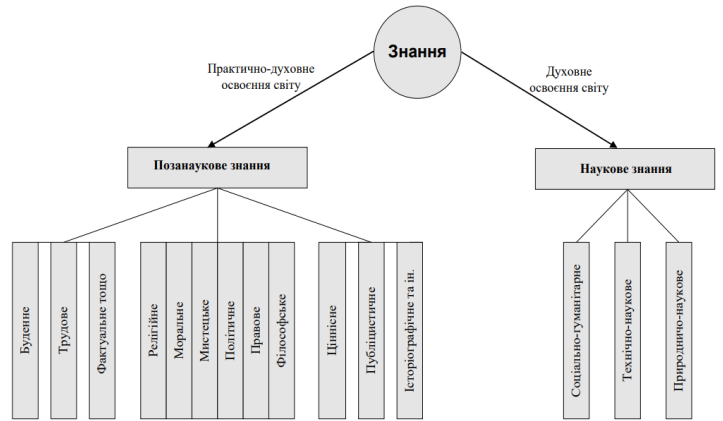
\includegraphics[scale=.5]{images/filosophy_diagram_1.png}
	\caption{Знання як система.}\label{fig:philosophy:knolage_as_a_system}
\end{figure}

Ближче до наукового знання знаходяться ціннісне, публіцистичне,
історіографічне та інші типи знання, для яких притаманне певне когнітивне
навантаження, котре «виводить» людину в зовнішній світ її суспільного і
природного буття. Це знання передає гносеологічні особливості чуттєвого,
емоційного пізнання, зверненого на об’єктивне значення предметів і явищ
світу, суспільних відносин тощо. Водночас воно вирізбляє і відтіняє не так
предмет сам по собі, як почуття індивіда, його переживання, упевненість,
переконання та ін.

А ось репрезентоване різними формами суспільної свідомості знання має
подвійну природу: з одного боку, йому притаманні суб’єктивний і ціннісний
аспекти відтворення світу, а з другого --- воно вибудовується за параметрами
науки з типовим для неї об’єктивним, системним, теоретичним відтворенням
дійсності. Сутність різниці позанаукового і наукового знання полягає в тому,
що останнє вироблене й організоване в науці як спеціально витвореній для
пізнавального відношення людини до світу формі знання. Тоді як інші форми
суспільної свідомості не є власне пізнавальними. Кожна з них виконує
особливу роль в осягненні світу: мистецтво транслює емоційний досвід
людства, мораль гармонізує взаємини між людьми, філософія задовольняє
насамперед їх світоглядні запити тощо. І хоча будь-яка з цих функцій
неможлива без конкретного й адекватного відтворення свого об’єкту як
предмету людських почуттів, стосунків, запитів тощо, «цей знаннєвий
компонент заверстаний в контекст специфічного призначення форми, яка
виконує непізнавальні функції. Кожна з них має відповідне наукове
відгалуження, що її вивчає: етика --- мораль, естетика --- мистецтво,
релігієзнавство --- релігію і т.ін., хоч кожна з цих наук з її пізнавальним
спрямуванням не може замінити форму свідомості, яка є предметом її
вивчення» [\textit{Горак Г.І. Філософія: Курс лекцій / Г.І. Горак. --- К.: Вілбор, 1997. ---
С.107}].

Отже, роль і значення науки в сучасному суспільстві беззастережні. Проте
необхідно також звернути увагу на такі типи знання, які здобуті не тільки
науковими засобами, але й позанауковими прийомами, мають відмінну від
наукової природу та існують поза межами науки. Вони відображають і
увиразнюють ті царини буття людини й світу (індивідуальний досвід, побутову
сферу, укорінені етнічні та інші традиції, сакральне, інтимне, трансцендентне
тощо), які через специфіку науки (її абстракцій, експериментальних методів,
раціонально-системних побудов та ін.) не охоплюються нею, або залишаються
недоступними для неї. Але це в жодному разі не означає, що в міру розвитку
наукового знання воно витіснятиме знання позанаукове. Обидві ці форми
знання і надалі співіснуватимуть одна з одною у тісній співзалежності й
динаміці, тобто вони обопільно зростатимуть, змінюватимуться,
розвиватимуться і трансформуватимуться.

Роль науки в сучасному суспільстві безумовна. Проте необхідно також
звернути увагу на такі типи знання, які здобуті не тільки науковими засобами,
але й позанауковими прийомами, мають відмінну від наукової природу та
існують поза межами науки. Вони відображають і увиразнюють ті царини буття
людини й світу (індивідуальний досвід, побутову сферу, укорінені етнічні та
інші традиції, сакральне, інтимне, трансцендентне тощо), які через специфіку
науки (її абстракцій, експериментальних методів, раціонально-системних
побудов та ін.) не охоплюються нею, або залишаються недоступними для неї.
Але це в жодному разі не означає, що в міру розвитку наукового знання воно
витіснятиме знання позанаукове. Обидві ці форми знання і надалі
співіснуватимуть одна з одною в тісній співзалежності й динаміці. Тобто вони
обопільно зростатимуть, змінюватимуться, розвиватимуться і
трансформуватимуться.

Щодо узалежнення філософського і наукового знання, то в контексті їх
єдності оригінальну концепцію систематизації наук запропонував у 1902 р.
засновник філософського прагматизму Ч. Пірс. З його погляду, систематизація
наук має відбуватися не на підставі їх ієрархізації, тобто підпорядкування
однієї окремої науки іншій. За основу має бути обраний принцип
пріоритетності впорядкування знання. Під цим оглядом розташована вище в
класифікації наука є пріоритетнішим типом упорядкування знання, ніж
наступні, оскільки розробляє загальні принципи, на яких засновані і які
реалізують інші науки. Обравши філософію як чинник упорядкування знання за
основу, Ч. Пірс структурує систему наук таким чином:

\begin{enumerate}[label=\Roman*]
	\item Математика.

	\item Філософія, яку розподілено на:
	\begin{enumerate}[label=\arabic*)]
		\item феноменологію;
		
		\item нормативну науку, а саме:
		\begin{enumerate}[label=2.\arabic*)]
			\item естетику;

			\item етику;
			
			\item логіку, яка своєю чергою складається з:
			\begin{enumerate}[label=\alph*)]
				\item філософської граматики:
				
				\item критичної логіки;

				\item методевтики (риторики)			
			\end{enumerate}
		\end{enumerate}
			
		\item метафізику.	
	\end{enumerate}

	\item Природничі науки.
\end{enumerate}

На думку Ч. Пірса, математика є вступом до наук, тому що її приписи
стосуються тільки загальних правил роботи думки. А ось філософія складається
з трьох частин ‒ феноменології, нормативної науки і метафізики. «Про речі тут
не йдеться взагалі. На відміну від цього філософія є виразом здатності людської
істоти до досвіду: порядку співвіднесення думки і світу. Причому це
співвіднесення стосується не тільки «пізнавального досвіду», а й діяльного
досвіду. Перша ж філософська дисципліна, феноменологія, є наукою про «речі
як вони являються нам». Друга частина філософії – нормативна наука – вивчає
те, як ми маємо вчиняти. Нарешті, третя частина філософії, метафізика, вивчає
те, що є реальним. У цій ієрархії, приміром, логіка спирається на принципи,
віднайдені в структурі досвіду етикою та естеткою. Загалом же, вся філософія
залежить від прозрінь феноменології, а та – від установлень математики.
Остання ж серед філософських дисциплін – метафізика – вже є перехідною
ланкою до природознавства» [\textit{Мінаков М.А. Питання досвіду в філософії Ч.С.
Пірса / М.А. Мінаков // Мультиверсум. Філософський альманах. – К.: Центр
духовної культури, – 2006. – № 55. ‒ С.17}]. Водночас подібна класифікація
залишає осторонь не тільки соціогуманітарне, але й технічно-наукове знання.
Адже Ч. Пірс пропонував її широкому загалу в той час, коли соціогуманітарне
знання не вважалося науковим, а технічне знання підпорядковувалося
природничо-науковому.

\subsection{Структура наукового знання.}
Надскладну загальну систему структуру
наукового знання утворюють не тільки різні галузі науки, але й види наукового
знання, його рівні та елементи тощо. Наука розподіляється на численні галузі
знання залежно від того, який аспект дійсності --- матеріальний, соціальний,
духовний --- досліджує. За предметом і методом пізнання часто досить умовно
виокремлюють науки про природу як природничі, про людину і суспільство ---
соціогуманітарні (соціальні), про техніку --- технічні. Природничі науки – це
передусім механіка, фізика, хімія, біологія, анатомія тощо. Кожна з цих наук
внутрішньо структурована. Наприклад, фізику утворюють фізична хімія,
біофізика, оптика, квантова фізика та інші галузі фізичного знання. Хімію ---
неорганічна, колоїдна, органічна, аналітична хімія та ін. Окрему групу щодо
природничих наук складають технічні науки --- технічна фізика, електроніка,
гірнича справа, програмування, прикладна механіка, прикладна математика
тощо. Виняткове місце серед сучасних наук посідає математика, яка
використовується всіма науками для вирішення різних пізнавальних завдань.
На особливу увагу також заслуговують і соціогуманітарні науки --- історія,
соціологія, психологія, педагогіка та ін. Адже саме вони досліджують проблеми
рефлексії, самопізнання науки. Сьогодні активно розвивається філософія науки,
яка досліджує загальні аспекти науково-пізнавальної діяльності, структуру й
динаміку знання, соціокультурні фактори піднесення науки, її логікометодологічні засади тощо.

За віддаленістю від практики науки іноді поділяють на фундаментальні та
прикладні. Фундаментальні галузі знання не мають прямої орієнтації на
практику. Прикладні ж передбачають безпосереднє застосування результатів
наукового пізнання для розв’язання практичних завдань. З огляду на це саме
технічні науки часто вважаються прикладними науками.

Галузі наукового знання сформувалися на підставі поділу праці в різних
царинах науки. Галузеве розмаїття наукового знання важко осягнути.
Рясногранні галузі наукового знання утворюють окремі науки (механіка
математика, логіка), їх об’єднання за певною предметною дійсністю
(природознавство, суспільствознавство), предметом і методом пізнання
(природничі науки, технічні науки, технологічні науки, гуманітарні науки),
наявними міжгалузевими зв’язками (комплексні, міждисциплінарні
дослідження) та ін. Щоб якось організувати галузі наукового знання в
структурну одноцілість, в сучасній науці їх об’єднують таким чином:
математика, логіка, природознавство, технонауки, соціальні науки, гуманітарні
науки.

Як види наукового знання вирізняють емпіричне, теоретичне і
метатеоретичне, атрибутивне, екзистенційне і релятивне, синтетичне і
аналітичне, дискурсивне й інтуїтивне, засновкове і вивідне, об’єктно-описове і
нормативно-методологічне, індивідуальне і суспільне, ціннісне і нормативне та
багато інших його форм.

А ще до структури наукового знання слід зарахувати його рівневу
організацію (емпіричне, теоретичне, метатеоретичне наукове знання) та різні
елементи ‒ протоколи спостережень, графіки, класифікації, факти, закони,
теорії, принципи, моделі, науково-дослідні програми, парадигми тощо.

Водночас у науці провадяться різні наукові дослідження, які
класифікуються за видами з огляду на поставлену мету, і способи і технології
наукового пізнання. Залежно від особливостей предмету пізнання і специфіки
дисциплінарної організації досліджень серед них виокремлюють три основних
види ‒ фундаментальні, прикладні та дослідно-конструкторські.

Загальна класифікація наук в Україні:
\begin{enumerate}
	\item Фізико-математичні науки
	\item Хімічні науки
	\item Біологічні науки
	\item Геологічні науки
	\item Технічні науки
	\item Сільськогосподарські науки
	\item Історичні науки
	\item Економічні науки
	\item Філософські науки
	\item Філологічні науки
	\item Географічні науки
	\item Юридичні науки
	\item Педагогічні науки
	\item Медичні науки
	\item Фармацевтичні науки
	\item Ветеринарні науки
	\item Мистецтвознавство
	\item Архітектура
	\item Психологічні науки
	\item Військові науки
	\item Національна безпека
	\item Соціологічні науки
	\item Політичні науки
	\item Фізичне виховання та спорт
	\item Державне управління
\end{enumerate}

В Україні класифікацію наук затверджено відповідно до організації
наукової діяльності головних наукових установ держави ‒ Міністерства освіти і
науки України, Національної академії наук України, державних галузевих
академій наук, громадських спеціалізованих академій, відомчих галузевих
академій (галузевих науково-дослідних інститутів ‒ НДІ), наукових товариств
(громадських спеціалізованих організацій), вищих навчальних закладів
(університетів, академій, інститутів, тематика досліджень в яких формується за
профілем ВНЗ, його факультетів і кафедр). Загальна класифікація наук під цим
оглядом наведена вище.

Запропоноване вище структурування сучасного наукового знання не
передбачає всеосяжності й вичерпності його конструювання. Водночас система
сучасного наукового знання має вибудовуватися в контексті осягнення
закономірностей його диференціації та інтеграції.

\subsection{Диференціація та інтеграція наукового знання.} Диференціація
наукового знання призводить до появи кількох наук, котрі детальніше й глибше
вивчають коло явищ, яке було предметом вивчення однієї з них.
Гносеологічним підґрунтям диференціації є аналітичні дослідження в науці, які
передбачають різнобічний розгляд ознак і властивостей досліджуваних
об’єктів. Соціологічна засада диференціації –розподіл праці, спеціалізація у
виробничій діяльності. Диференціація розгортається в системі професійної
підготовки, в освіті та передбачає збільшення професій вузького профілю,
наявність мережі спеціалізованих навчальних закладів різних рівнів тощо.
Диференціація наукового знання дозволяє більш глибоко вивчити, окремі
аспекти дійсності. Вона полегшує працю вчених, впливає на структуру
наукового співтовариства.

Зворотний до диференціації процес інтеграції наукового знання передбачає
об’єднан\-ня в одноцілість будь-яких окремих, раніше ізольованих його видів,
рівнів, елементів. Інтеграція наукового знання полягає у взаємному прониканні
методів дослідження з одних наук в інші, у виробленні спільного для низки
наук підходу до вивчення, теоретичного опису й пояснення явищ. До того ж
інтеграція наукового знання розгортається не тільки в межа якоїсь окремої
наукової галузі. Нагадаємо, що нині налічується не менше 15 тисяч різних
наукових дисциплін. Поряд з галузевими, дисциплінарними, достатньо
вузькими дослідженнями на перший план все більше висуваються міжгалузеві,
міждисциплінарні і проблемно-орієнтовані форми дослідницької діяльності.
Цьому значною мірою сприяє широке застосування в різних науках методів
математики. А ось інтеграція природничих і сусп. наук, яка складається в
процесі здійснення науково-технічних і соціально-економічних програм,
спирається на застосування не тільки математичних, але й загальнологічних
методів пізнання.

В основі вирішення проблеми інтеграції наукового знання лежить
філософський принцип єдності світу. Оскільки світ єдиний, його адекватне
відображення має репрезентувати єдність, одноцілість, взаємну залежність
речей і явищ. У природі немає абсолютних розмежувальних ліній. Тому її
одноцілість відтворюється в системній природі природничо-наукового знання.
Коли вивчатимете проблеми змін, руху, розвитку світу, так само зверніть увагу
на лише відносну самостійність форм руху матерії, які розгортаються одна
через одну, переходять одна в одну. Також тісно узележненими між собою
виявляються різні форми соціального і духовного світу.

Механізм інтеграції наукових знань зумовлений співзалежністю форм руху
матерії, єдністю історичного й логічного тощо. Дія механізму інтеграції може
відбуватись в різних процесах. Для синтезу наукових знань є чотири основні
форми дії механізму інтеграції:
\begin{itemize}
	\item внутрішня: взаємне проникнення напрямів, яке відбувається в кожній
	окремій галузі науки;

	\item зовнішня: взаємний зв’язок, єдність між галузями знання, утворення
	комплексів, які належать до єдиної системи науки;

	\item вертикальна: інтегруючий уплив наук від більш загальних, теоретичних
	(філософія, кібернетика) до «проміжних» (природничі, суспільні), а відтак до
	прикладних, технічних, безпосередньо пов’язаних з виробництвом;
	
	\item горизонтальна: зв’язок наукових галузей усередині великих і давно
	існучих комплексів наук (суспільних, природничих, технічних).
\end{itemize}

Отож, як наслідок відображення в інтеграціних процесах сучасної науки
складних ланок єдиного ланцюга руху й розвитку дійсності з’являються
«порубіжні», «пограничні» наукові знання. Вони виникають переважно на
«стику» наук і мають такі риси:

\begin{itemize}
	\item постають складовими ланками єдиного ланцюга розгортання наукового
	знання конкретних наук, які вивчають їх і яким притаманна не абсолютна, а
	лише відносна самостійність;
	
	\item розробляють і використовують міждисциплінарні наукові методи, які
	можуть застосовуватися в різних науках (математичний метод, комп’ютерний
	експеримент тощо);

	\item перебувають у пошуку об’єднавчих теорій і принципів, до яких можна
	було б звести нескінченну різмаїтість явищ світу (єдина теорія поля,
	глобальний еволюційний синтез в біології, фізиці хімії та ін.);

	\item обґрунтовують теорії, які синтезують наукові знання з різних дисциплін,
	об’єдную\-чи низку далеко віддалених одна від одної наук, і виконують
	методологічні функції в науці, насамперед у природознавстві (кібернетика,
	синергетика);

	\item змінюють принципи виокремлення наукових дисциплін.
\end{itemize}

Отже, диференціація наукового знання передбачає його інтеграцію, і
навпаки. Водночас диференціація та інтеграція наукового знання не призводять
ні до повного відокремлення наук, які виникли внаслідок диференціації, ні до
втрати конкретними науками їх специфіки внаслідок розгортання тенденції до
інтеграції. Як не є, але посилення інтегративних тенденцій у сучасній науці
сприяє підвищенню інтересу до проблеми інтеграції та диференціації наукового
знання у вітчизняній та іноземній літературі.

Основна література: 1-4, 7-10.

Додаткова література: 14-19, 37-38, 48-49, 65, 77, 82-83, 86, 102, 106, 112-
113, 116.

\section{Моделювання наукового пізнання}

\textbf{Тема:} Основні моделі наукового пізнання

\textbf{Мета розгляду теми} ‒ вивчення різних моделей розвитку науки для
опанування методологією моделювання філософських і наукових досліджень.

\textbf{Основні поняття:} модель, кумулятивність знання, кумулятивізм, наукова
революція, фальсифікація знання, елімінація знання, науково-дослідницька
програма, наукова парадигма, еволюціонуюча раціональність, методологічний
анархізм.

\textbf{План:}
\begin{enumerate}
	\item Кумулятивні моделі розвитку науки і наукового пізнання.
	\item Діалектико-матеріалістична модель наукового пізнання.
	\item Логічні моделі наукового пізнання.
	\item Соціокультурні моделі наукового пізнання.
\end{enumerate}

\subsection{Кумулятивні моделі розвитку науки і наукового пізнання.} В
сучасному філософському і науковому дискурсі проблема моделювання
філософських і наукових досліджень репрезентована переважно під оглядом
протиставлення кумулятивних і некумулятивних концепцій розвитку науки
(пригадайте, як розвивалася наука в духовному поступі людства за попередньо
опрацьованою темою).

Суть кумулятивної концепції полягає в тому, що одного разу обґрунтовані
наукою знання про реальні властивості, зв’язки, процеси, явища природи і
суспільства накопичуються, акумулюються, утворюючи своєрідний постійно
зростаючий фонд, який безперервно збільшується, що зумовлює піднесення та
розвиток знання. З огляду на це кумулятивна концепція моделювання
філософських і наукових досліджень розгортається на таких методологічних
засадах:
\begin{itemize}
	\item в науці наявні раз і назавжди встановлені, остаточні, незмінні істини, які
	постійно накопичуються;

	\item помилки не є елементами наукового знання і не становлять жодного
	інтересу для історії і методології науки та провадження наукових досліджень;

	\item наука жорстко відокремлена від ненаукових форм знання, так само й від
	філософії та інших форм духовності;
	
	\item увесь накопичений історією науки запас знань залишається без змін: ніщо
	не відкидається, прообраз і витоки нового завжди можна знайти в старому
	знанні, що відтворено у відомому висловлюванні: «нове –добре забуте старе».
\end{itemize}

Кумулятивна природа знання – давно відомий факт. Наприклад, Аристотель
в IV ст. до н.е. описав близько 500 видів тварин. А французький дослідник
природи XVIII віки К. Бюффон у 36-томній праці «Природна історія»
репрезентував уже десятки тисяч видів тварин. У наш час у науковій літературі
зафіксовано понад півтора мільйони видів. Як атрибут знання кумулятивність
разом з іншими властивостями розкриває насамперед його історичний
розвиток. Вона фіксує соціальність науки і наукового прогресу, а також той
факт, що в науці підсумовуються зусилля не одного покоління учених. Крім
того, кумулятивність свідчить і про таку важливу особливість наукового
знання, як спадкоємність і незворотність наукової творчості. Отже, розвиток
наукового знання передбачає значущість суми зусиль усіх поколінь учених.
Французький математик А. Пуанкаре, роздумуючи про науку, зазначав, що
«вона є колективною творчістю і не може бути нічим іншим; вона як
монументальна споруда, будувати яку треба віки і де кожен повинен принести
камінь, а цей камінь часто коштує йому цілого життя. Отже, вона дає нам
почуття необхідної кооперації, солідарності наших зусиль із зусиллями наших
сучасників і наших наступників» [\textit{Пуанкаре А. Про науку / А. Пуанкаре. --- М.,
1983. --- С.510}].

Кумулятивність знання --- лише початковий пункт і фундамент розуміння
розвитку науки. Проте від об’єктивної властивості кумулятивності слід
відрізняти концепцію, яка прагне пояснити розвиток науки тільки власне
кумулятивністю. Подібний кумулятивізм не пояснює і не враховує багато
важливих моментів реальної науки. Насамперед незрозумілою для нього
залишається динамічність її минулого, закономірності розвитку науки як
одноцілої системи, еволюція та зміна її структури. Крім того, кумулятивізм не
пояснює, як відбуваються переоцінка і якісний відбір знань, які постійно
накопичуються. У ньому відсутня процедура критики, заперечення, виявлення
суперечностей нового і старого знання. Водночас реальна історія науки
свідчить про те, що її розвиток ‒ це не лише накопичення, але й постійне
заперечення, відкидання, критичне подолання ідей, гіпотез, теорій, методів
пізнання тощо.

Класичним прикладом кризи кумулятивістської моделі науки є так звана
криза в підставах математики початку XX століття. Саме математики були
переконаними прибічниками класичної кумулятивістської епістемології,
репрезентуючи власну науку як ідеал чіткого доведеного і неспростовного
знання. Водночас відомі з гіркотою висловлені щодо цього слова видатного
математика Д. Гільберта, які прозвучали в 1925 р.: «Подумайте: в математиці –
цьому зразку достовірності й істинності – утворення понять та хід висновків, як
їх кожний вивчає, викладає і застосовує, призводить до безглуздостей. Де ж
шукати надійність та істинність, якщо навіть суто математичне мислення дає
осічку»? [\textit{Гільберт Д. Підстави геометрії / Д. Гільберт. --- М.-Л.: Гостехиздат,
1948. --- С.349}]. Та незважаючи на це, учений вперто продовжував шукати
«остаточне» обґрунтування математики, звертаючись, зокрема, до чуттєвої
наочності як гаранта абсолютної непогрішності математичних виводів.
Програма виявилася нездійсненною… Мало того, австрійський математик і
логік К. Гедель довів (теореми 1932 і 1934 рр.) неспроможність ідеї повного й
остаточного обґрунтування математики, та й загалом повної формалізації
наукового знання. Але це означало, що «криза торкнулася не власне
математики, яка продовжувала розвиватися, а кумулятивної методології, яку
необхідно було переглянути, що й було здійснено надалі» [\textit{Черняк B.C.
Особливості сучасних концепцій розвитку науки / B.C. Черняк // У пошуках
теорії розвитку науки / В.Н. Порус, A.JI. Никифоров. --- М.: Наука, 1982. --- С.16-
25}]. Обмеженість кумулятивних концепцій науки полягає ще й в тому, що з
поля зору випадає проблема наукової творчості, здійснення наукового
відкриття. Якщо ж абсолютизувати ідею соціальної природи науки, то можна
прийти до заперечення ролі окремих учених, а наукове дослідження зобразити
як анонімний науковий процес. Нарешті, слід зазначити, що в рамках цієї
концепції відсутній механізм передбачення і прогнозування майбутнього
розвитку науки.

\subsection{Діалектико-матеріалістична модель наукового пізнання.} У створеній
К. Марксом і Ф. Енгельсом діалектико-матеріалістичній філософії
пропонувалася певна теоретична модель розвитку науки, яка спиралася на
концепцію наукової революції. Власне наукова революція розумілася, поперше, як якісна зміна в системі знання і мислення, що потребує зміни стратегії
наукового пошуку; по-друге, як докорінна перебудова системи пізнавальної
діяльності, якісний стрибок у способах виробництва знання. Особливе значення
для розуміння підґрунтя і гносеологічної природи філософських і наукових
досліджень мають розвідки Ф. Енгельсом становлення й розвитку
дисциплінарного природознавства XVIII-XIX ст. та ленінський розгляд
новітньої революції в природознавстві в кінці XIX --- на початку XX ст.
Незважаючи на те, що В. Ленін виходив з украй ідеологізованих позицій
марксизму, використання великої кількості робіт видатних учених-дослідників
природи, а також зарубіжних істориків науки дозволило йому отримати
методологічно значущі висновки про природу наукової революції. Тому радимо
обов’язково опрацювати гл. 5. «Новітня революція в природознавстві та
філософський ідеалізм» з праці В. Леніна «Матеріалізм та емпіріокритицизм»
[\textit{Ленін В.І. матеріалізм та емпіріокритицизм / В.І. Ленін // Повне зібр. творів.
--- Т.18. --- К.: Політвидав України, 1961. --- 490 с.}].

У радянський період розвитку філософії марксизму такі дослідники, як Б.
Кедров, B. Стьопін, П. Гайденко, В. Казютинський та інші здійснили
філософський розгляд природи наукової революції, її структури, механізмів,
цілей, рушійних сил, філософсько-світоглядних і соціально-історичних засад.
Українські філософи П. Дишлевий, О. Кедровський, М. Тарасенко та інші за
зовнішніми процесами в науці виявили фундаментальні перетворення, котрі
відбуваються в ній, викликаючи і забезпечуючи такі її внутрішні революційні
зміни, які викликають зміни картини світу. До них належать зміни
філософських передумов і підстав науки; переоцінка гносеологічної природи
науки, пізнавальних можливостей її теорій, об’єктивної значущості її понять,
законів, принципів; нарешті, принципові зміни філософських позицій науковців
як дослідників природи.

Тим, кого зацікавлять проблеми розгортання наукових революцій в
духовному поступі людства, радимо прочитати праці російського філософа B.
Степіна, який виокремив чотири глобальні революції в історії природознавства.
Зверніть увагу на їх основні характеристики, наведені нижче.

Перша революція. XVII --- перша половина XVIII ст. --- становлення
класичного природознавства. Основні характеристики: механістична картина
світу як загальнонаукова картина реальності; об’єкт --- мала система як
механічний пристрій із жорстко детермінованими зв’язками, властивість цілого
повністю визначається властивостями частин; суб’єкт і процедури його
пізнавальної діяльності повністю вилучаються із знання для досягнення його
об’єктивності; пояснення як пошук механічних причин і сутностей, зведення
знань про природу до принципів та уявлень механіки.

Друга революція. Кінець XVIII --- перша половина XIX ст. --- перехід
природознавства в дисциплінарно організовану науку. Основні характеристики:
механістична картина світу перестає бути загальнонауковою, формуються
біологічні, хімічні та ін. картини реальності, які не зводяться до механістичної
картини світу; об’єкт розуміється відповідно до наукової дисципліни не лише в
поняттях механіки, але й таких як «річ», «стан», «процес», що припускає
розвиток і зміну об’єкта; суб’єкт має бути елімінований із результатів пізнання;
виникає проблема розмаїтості методів, єдності й синтезу знань, класифікації
наук; зберігаються загальні пізнавальні установки класичної науки, її стилю
мислення.

Третя революція. Кінець XIX --- середина XX ст. --- перетворення параметрів
класичної науки, становлення некласичного природознавства. Істотні події:
генезис і розвиток релятивістської і квантової теорій у фізиці, становлення
генетики, квантової хімії, концепції нестаціонарного Всесвіту, виникають
кібернетика і теорія систем. Основні характеристики: наукова картина світу, що
розвивається, порівняно (відносно) істинне знання; інтеграція
частковонаукових картин реальності на підставі розуміння природи як складної
динамічної системи; об’єкт --- не стільки «собітотожна річ», скільки процес із
стійкими станами; співвіднесена об’єкта із засобами і операціями діяльності;
складна динамічна система, стан цілого станів його частин, які не зводяться до
суми, що розвивається; імовірнісна причиновість замість жорсткого,
однозначного зв’язку; нове розуміння суб’єкта як такого, що перебуває
усередині, а не поза спостережуваним світом --- необхідність фіксації умов і
засобів спостереження, обчислення способів постановки питань і методів
пізнання, залежність від цього розуміння істини, об’єктивності, факту,
пояснення; замість єдиної істинної теорії допускається декілька, котрі містять
елементи об’єктивності теоретичних описів одного й того самого емпіричного
базису.

Четверта революція. Кінець XX --- початок XXI ст., радикальні зміни в
підставах наукового знання і діяльності --- народження нової
постнеклассической науки. Події --- комп’ютеризація науки, ускладнення
приладових комплексів, зростання міждисциплінарних досліджень,
комплексних програм, зрощення емпіричних і теоретичних, прикладних та
фундаментальних досліджень, розробка ідей синергетики. Основні
характеристики: наукова картина світу --- взаємодія різних картин реальності;
перетворення їх на фрагменти загальної картини світу, взаємодію шляхом
«парадигмальних щеплень» ідей з інших наук, стирання жорстких
розмежувальних ліній; на передній план виходять унікальні системи --- об’єкти,
які характеризуються відкритістю і саморозвитком, об’єкти, котрі історично
розвиваються та еволюційно перетворюються, «людиномірні» комплекси;
знання про об’єкт співвідносяться не лише із засобами, але й з ціннісноцільовими структурами діяльності; усвідомлюється необхідність присутності
суб’єкта, що увиразнюється передусім ув тому, що включаються аксіологічні 
чинники в пояснення, а наукове знання з необхідністю розглядається в
контексті соціального буття, культури, історії як нероздільне з цінностями та
світоглядними установками, що загалом зближує науки про природу і науки
про культуру [\textit{Степин В.С. Философия науки. Общие проблемы: учебник для
асп. и соиск. уч. ст. канд. наук / В.С. Степин. – М.: Гардарики, 2006. ‒ С.308-
330}].

Намагаючись пристосувати марксизм до реалій ХХ століття і виступаючи
проти емпіризму який завдає шкоди сучасній науці, філософ-неомарксист Л.
Альтюсер запропонував концепцію наукового пізнання як синтетичної
переробки колишнього знання. Спираючись на дослідження французьких
істориків науки та епістемологів А. Койре, Г. Башляра, Ж. Кангійєма процес
французький філософ намагався зобразити процес наукового пізнання як
перехід від «поганих» абстракцій до «хороших». Особливу увагу Л. Альтюсер
звернув на наукові революції --- генезис математики в Стародавній Греції,
формування класичної фізики XVII-XVIII ст., створення науки про суспільство
К. Марксом, --- пояснюючи їх як стрибкоподібний перехід до нової
«проблематики», під якою малося на увазі структуроване поле проблем, котре
зумовлює саму можливість їх постановки. Відповідно до цього в двотомній
роботі «Читати «Капітал» (1965), написаній разом з учнями (У. Балібаром, Д.
Лекуром, П. Реймоном та ін.), Л. Альтюсер зобразив наукову революцію
Маркса як перехід від одноплощинної емпіричної проблематики
переднаукового знання до багаторівневої, структурованої проблематики
справжньої науки. Л. Альтюсер також запропонував «антигегельянську»
інтерпретацію «Капіталу» Маркса, по-своєму розробив питання про роль
філософії в науковому пізнанні тощо.

У ще одного відомого філософа-неомарксиста Г. делла Вольпе філософія
зводиться до методології пізнання. Ним ставилося завдання надати історичному
матеріалізму чіткої наукової форми. Дослідивши різні варіанти вирішення
проблеми загального і особистісного в історії філософії, Г. делла Вольпе
дійшов висновку про непридатність філософських абстракцій для конкретнонаукової роботи. З його погляду, потрібна «специфічна логіка специфічного
предмета», яка використовує особливі, «визначені» абстракції. Завдання
філософії --- розробка методу отримання таких абстракцій як способу руху від
конкретного до абстрактного і в зворотньому напрямі.

Отже, представники марксизму і неомарксизму створили досить
продуктивну, хоча й незавершену діалектико-матеріалістичну модель
філософських і наукових досліджень, яка мала істотний вплив на розвиток наки
ХХ ст.

\subsection{Логічні моделі наукового пізнання.} У сучасній західній філософії науки
можна умовно виокремити два основні напрями розробки теоретичних моделей
філософських і наукових досліджень. Один з них орієнтується на їх логічне
моделювання за допомогою нормативних принципів логічної природи,
(К. Поппер, І. Лакатос та ін.). Другий напрям прагне розробити соціокультурну
та соціопсихологічну моделі філософських і наукових досліджень (Т. Кун, С.
Тулмін, Дж. Холтон та ін.).

Як вважає К. Поппер, для того, щоб зберегти емпіричну природу і не
перетворитися на метафізичну догму, наука має постійно розвиватися. Отож, у
наукових дослідженнях повинні безперервно висуватися нові теорії та
відбуватися їх перевірка і спростування. Якщо ж цей процес припиняється і
деякі теорії панують протягом тривалого часу, то вони перетворюються на
неспростовні метафізичні системи. Наука прогресує завдяки сміливим ідеям,
висуненню нових, усе більш дивних теорій (наприклад, геліоцентричної,
імовірності тощо) і спростуванню колишніх теорій. В науці ніколи не існує
достатніх підстав для упевненості в тому, що вже досягнуто істини. Те, що
називається «науковим знанням» переважно не є знанням у платонівсько -
аристотелівському сенсі, а, швидше, --- інформацією, яка стосується різних
суперечливих гіпотез та способу, за допомогою якого вони витримують різні
перевірки [\textit{Поппер К. Відкрите суспільство і його вороги / К. Поппер. – Т. II. –
М., 1992. – С.20-21}].

На думку К. Поппера, емпіричний базис не є чимось остаточно істинним, як
вважали неопозитивісти. Він --- продукт конвенції, залежної від відповідної
теорії. Раціонально діє той учений, який будує сміливі теоретичні гіпотези,
відкриті розмаїтим спробам їх спростування. Синонімом раціональності є
безкомпромісна критика, яка ґрунтується на принципі фальсифікації. Отож,
теорія, котра не може бути спростована будь-якою мислимою подією не є
науковою. Неспростовність є не гідністю теорії, як часто й безпідставно
вважається, а її недоліком. Наслідком спростовності тверджень є визнання
принципової гіпотетичності, передпозитивності знання, оскільки претензія
знання на абсолютну істинність суперечить принципу критицизму, а, відтак є
нераціональною.

Зростання наукових знань --- це процес, який «іде від старих проблем до
нових за допомогою припущень і спростувань» [\textit{Поппер К.Р. Логика и рост
научного знания. Избр. работы / Пер. с англ. / К.Р. Поппер. – М.: Прогресс,
1983. – С.121}]. Його сутністю є природний відбір гіпотез: знання завжди
складається із сукупності тих гіпотез, які доводять певну здатність виживати в
боротьбі за існування. Елімінує нездатні вижити гіпотези конкуренція. Отже,
пізнання – це процес зменшення незнання за допомогою елімінації помилкових
суджень, оскільки надійних джерел отримання істини немає і жодна теорія не
може бути безумовно підтвердженою. Тому завдання вчених – знаходити
помилки й усувати їх за допомогою чіткої перевірки теорії та висунення нових
гіпотез.

З погляду К. Поппера, в процесі зростання наукового знання стара теорія
завжди відкидається. І чим більше нова теорія відрізняється від колишньої тим
навіть краще, бо це робить її більш сміливою, а отже й такою, що більше
фальсифікується. Проте ідея елімінації («вбивства», за термінологією філософа)
старих теорій є суперечливою і не задовольняє принципові спадкоємності в
розвитку знань. Адже наукові знання хоча й «мутують» та схильні до
«природного відбору» (як і генетичний матеріал) водночас не можуть
відірватися від накопичених історією розвитку науки досягнень. Тому з появою
нових теорій більш глибокі й загальні старі теорії, якщо вони розгортали
істинне знання, залишаються в науці і продовжують використовуватися в ній
(наприклад, теорія А. Ейнштейна не призвела до загибелі законів І. Ньютона).
Як правило, зв’язок між теоріями підкоряється принципу відповідності.

За К. Поппером, зміст наукового знання може змінюватися як завгодно:
жодних закономірностей, тенденцій, напрямів, які визначають, як відбувається
цей процес не передбачається. Як стверджує сам філософ, наукове знання в
процесі зростання ускладнюється і одного дня наукові проблеми можуть стати
настільки складними, що мислення людини виявиться не в змозі впоратися з
ними. Але філософа це не дуже турбує, оскільки він розглядає знання як
особливий – третій світ, як світ ідей, проблем, теорій, який існує немов би
самостійно разом зі світом фізичних об’єктів і світом свідомості людини.
Водночас другий і третій онтологічні світи відповідають так званому
суб’єктивному і об’єктивному мисленню. Суб’єктивне мислення – це акти
сприйняття або розумові процеси свідомості, об’єктивне мислення – результати
розумових процесів і актів сприйняття, або їх зміст. Світ розумових процесів і
світ їх реультатів різні по суті. Якщо суб’єктивне мислення допускає причинові
зв’язки між своїми актами, то об’єктивне мислення – зв’язки логічної природи.
Відтак теорія постає об’єктом вивчення, річчю, якою людина намагається
оволодіти. Але головним завданням епістемології К. Поппер уважав вивчення
об’єктів «третього світу».

Реалізація попперівської моделі зростання наукового знання натрапила на
серйозні труднощі, пов’язані з абсолютизацією принципу фальсифікації;
конвенціалізмом у трактуванні вихідних підстав знання; відривом об’єктивного
знання від історично конкретного суб’єкта, що пізнає; відмовою визнання
об’єктивної істинності наукового знання; недооцінкою соціокультурних
чинників розвитку знання; перебільшенням аналогії з біологічною еволюцією;
запереченням наявності певних закономірностей в розвитку науки, природи і
суспільства; перебільшенням інтенсивних аспектів у розвитку знання. Отже,
поставивши низку важливих для розгортання наукового дослідження проблем ---
зростання наукового знання, ролі гіпотез у розвитку науки, ролі емпіричного
спростування і теоретичної критики в розвитку нового знання, співзалежності
старих та нових теорій тощо --- К. Поппер не зміг остаточно їх вирішити.

Якщо К. Поппер вважав, що процес зростання наукових знань має тільки
дискретну природу й відбувається шляхом перманентних революцій, то його
учень і послідовник І. Лакатос у власній моделі філософських і наукових
досліджень намагався врахувати безперервні моменти в розвитку наукових
знань. Це знайшло відображення у його концепції науково-дослідницьких
програм.

Основною проблемою для І. Лакатоса виявилося пояснення значної
стійкості та безперервності наукової діяльності --- того, що Кун називав
«нормальною наукою». Концепція К. Поппера не давала такого пояснення,
оскільки вважалося, що вчені повинні фальсифікувати і негайно відкидати
будь-яку теорію, яка не узгоджується з фактами. З погляду І. Лакатоса, така
позиція є «наївним фальсифікаціонізмом» і не відповідає показникам історії
науки, котрі свідчать, що теорії можуть існувати і розвиватися, незважаючи на
наявність великої кількості «аномалій» (фактів, що їм суперечать). Цю
обставину можна пояснити, на думку І. Лакатоса, якщо порівнювати з емпірією
не одну ізольовану теорію, а серію теорій, котрі змінюються, пов’язаних між
собою єдиними засадничими принципами. Таку послідовність теорій він і
назвав науково-дослідницькою програмою. Подібна програма – це
метатеоретичне утворення, в межах якого здійснюється теоретична діяльність;
це сукупність теорій, які змінюють одна одну та об’єднуються визначеною
сукупністю засадничих ідей і принципів. Розвиток науки, за І. Лакатосом, є
послідовною зміною науково-дослідницьких програм, які можуть деякий час
існувати або конкурувати одна з одною [\textit{Лакатос И. Методология научных
исследовательских программ / И. Лакатос // Вопросы философии. – М., 1995. –
№ 4. ‒ С.147}].

Структура науково-дослідницької програми містить «жорстке ядро»,
«захисний (або запобіжний) пояс» і систему методологічних правил
(«евристик»). «Жорстке ядро» науково-дослідницької програми – те, що є
загальним для всіх її теорій, сукупність тверджень, котрі у рамках цієї
дослідницької програми приймаються (внаслідок конвенції) як неспростовні.
Це найбільш загальні уявлення про реальність, яку описують теорії, які входять
у програму; основні закони взаємодії елементів цієї реальності; головні
методологічні принципи, пов’язані з цією програмою. Наприклад, в ядро
ньютонівської науково-дослідницької програми входять уявлення про те, що
реальність складається з корпускул, які рухаються в абсолютному просторі й
часі.

«Захисний пояс» – сукупність допоміжних теорій і гіпотез, інваріантом яких
є «жор\-стке ядро». Він переймає на себе вогонь критичних аргументів та
оберігає ядро науково-дослідницької програми від фальсифікації, від
спростовуючих фактів.

«Евристики» – методологічні правила, одні з яких визначають, яких шляхів
дослідження слід уникати (негативні евристики), а другі ‒ яким шляхом
слідувати (позитивні евристики) в межах цієї науково-дослідницької програми.
Позитивна евристика складається з правил, які сприяють позитивному розвитку
програми. Це певна стратегія вибору першочергових проблем і завдань, котрі
повинні вирішувати учені. Наявність позитивної евристики дозволяє певний час
ігнорувати критику та аномалії і займатися конструктивними дослідженнями.
За наявності такої стратегії, вчені мають право маніфестувати одержання
незрозумілих і таких, що потенційно спростовують програму фактів, а також,
що їх існування не є приводом для відмови від програми. 

Метою науки, з погляду І. Лакатоса, є захист «жорсткого ядра». Тому й
зміна теорій значною мірою залежать від взаємин «жорсткого ядра» і
«захисного поясу» та одночасно не дуже залежить від емпіричної дійсності. В
розвитку науково-дослідницької програми можна виокремити два етапи –
прогресивний (програма прогресує, коли її теоретичне зростання передбачає
відкриття емпіричних фактів) і регресивний (виродження) – теоретичні
узагальнення відстають від зростання емпіричних фактів. На прогресивній
стадії «позитивна евристика» здатна стимулювати висунення допоміжних
гіпотез, які розширюють зміст програми. В рамках програми, яка успішно
розвивається, вдається розробляти все більш досконалі теорії, котрі пояснюють
усе більше й більше фактів. Саме тому вчені схильні до стійкої позитивної
роботи в межах подібних програм і припускаються певного догматизму щодо їх
засадничих принципів.

Проте це не може тривати нескінченно довго. Досягнувши так званого
«пункту насичення», розвиток науково-дослідницької програми різко
гальмується, евристична сила програми починає слабшати, і перед ученими
виникає питання про те, чи варто продовжувати працювати в її рамках. Зростає
кількість несумісних фактів, з’являються внутрішні суперечності, парадокси.
Водночас наявність подібних симптомів ще не може слугувати об’єктивною
підставою для відмови від науково-дослідницької програми. Така підстава, на
думку І. Лакатоса, виникає тільки з появою нової науково-дослідницької
програми, яка пояснює емпіричний успіх своєї попередниці та витісняє її
подальшим проявом евристичної потужності, здатності теоретично передбачати
невідомі раніше факти.

Процес витіснення прогресуючими науково-дослідницькими програмами
своїх по\-пе\-ред\-ниць, якіо вичерпали внутрішні ресурси розвитку, І. Лакатос
називає науковою революцією. Як їх наслідок, старі науково-дослідницькі
програми зникають безслідно. Проте вчений не розглядає процес зародження
нових науково-дослідницьких програм, критерії оцінки їх прогресивності,
припускаючи, що це питання виходить за межі методології науки.

Зазвичай, у будь-якій науковій дисципліні є декілька альтернативних
науково-дос\-лідницьких програм. Конкуренція між ними, взаємна критика,
чергування періодів розквіту і занепаду таких програм надають розвитку науки
той реальний драматизм наукового пошуку, який відсутній в кунівській
монопарадигмальній «нормальній науці». Отже, модель філософських і 
наукових досліджень І. Лакатоса додає нові моменти до розуміння розвитку
наукового знання, зокрема щодо питання про його спадкоємність. Проте вона
вирішує його тільки в межах еволюційних періодів розвитку науки, тоді як
питання про спадкоємність під час зміни програм залишається відкритим. Крім
того, науково-дослідницька програма не відображає впливу соціокультурних
чинників на процес розвитку науки. Водночас запропонована філософом
методологія виявилася продуктивною щодо історико-наукових досліджень
деяких конкретних періодів розвитку науки.

\subsection{Соціокультурні моделі наукового пізнання.} Модель історичної
динаміки філософських і наукових досліджень Т. Куна сформувалася в
полеміці з логічним емпіризмом неопозитивістів і критичним раціоналізмом К.
Поппера. Т. Кун запропонував відмовитися від пануючого в цих напрямах
образу науки як системи знань, зміна й розвиток якої підпорядковуються
законам методології і логіки. З його погляду, необхідно замінити цей образ на
розуміння науки як діяльності наукових співтовариств, яка залежить від
культури, історії, соціальної організації, психологічної і технічної бази тощо.
Тому, не тільки на противагу кумулятивістам, але й тим ученим, які
обґрунтовували логічні моделі динаміки наукового знання, філософ описав її як
послідовність періодів кумулятивного розвитку, який переривається
некумулятивними стрибками – науковими революціями. Основними періодами
цього процесу є:
\begin{itemize}
	\item початкова допарадигмальна стадія розвитку науки, якій притаманна
	наявність різних поглядів, фундаментальних теорій, загальновизнаних методів і
	цінностей;
	
	\item створення єдиної парадигми на підставі консенсусу членів наукового
	співтовариства;

	\item на підґрунті цієї парадигми здійснюється нормальний розвиток науки,
	накопичуються факти, вдосконалюються теорії і методи;

	\item під час такого розвитку виникають аномальні ситуації, які призводять до
	кризи, а відтак до наукової революції;

	\item наукова революція як період розпаду парадигми, конкуренція між
	альтернативними парадигмами і, зрештою, затвердження нової парадигми.
\end{itemize}

Отже, стрижневим терміном концепції Т. Куна є поняття наукової
парадигми як системи норм, засадничих теоретичних поглядів, методів,
фундаментальних фактів і зразків діяльності, які визнаються і сповідуються
всіма членами певного наукового співтовариства як логічного суб’єкта наукової
діяльності. Поняття парадигми є корелятивним щодо поняття наукового
співтовариства. Ученого, згідно з Т. Куном, можна зрозуміти як такого тільки
за його приналежністю до наукового співтовариства, члени якого
дотримуються певної парадигми. Створення парадигми означає досягнення
згоди стосовно питання про загальні зразки теоретичних та емпіричних знань,
дослідницької методології. Як правило, парадигма втілюється в класичних
працях учених і підручниках і на багато років визначає коло проблем та методів
їх вирішення в тій або тій галузі науки. Тому більшість учених звільнена від
роздумів про найбільш фундаментальні питання власної дисципліни: вони вже
«вирішені» парадигмою. Тому головна увага вчених спрямовуються на
розв’язання невеликих конкретних проблем («головоломок»).

Проте, здійснюючи парадигмальну діяльність і очікуючи на немов би
«передбачені» парадигмою факти, вчений іноді виявляє дещо несподіване –
аномалію, тобто розбіжність між емпіричними фактами і схемою,
запрограмованою парадигмою. Т. Кун детально аналізує виникнення наукових
аномалій, які призводять до заміни старої парадигми. Парадигма «вибухає»
зсередини під тиском «аномалій», котрі не мають права на існування в її межах.
Спочатку виникає криза і екстраординарна наука, потім щось подібне до
парадигмального періоду. Під час його розгортання посилюється увага до
філософських засад науки. Відкриття аномального факту – це процес, початок
якого пов’язаний з прагненням зберегти стару парадигму. Його завершення
знаменує перехід до нової парадигми. Усвідомлення аномалій як стимулююча
зміна парадигм є внутрішнім механізмом розвитку знань.

Наукова революція настає тоді, коли створюються нові парадигми. Вони
формуються, як правило, вченими-аутсайдерами, які стоять поза «школою», і їх
активною діяльністю щодо пропаганди власних ідей. Процес наукової
революції виявляється в Т. Куна стрибкоподібним відбором за допомогою
конфлікту наукових співтовариств, згуртованих одноцілим «поглядом на світ».
Остаточним підсумком такого відбору є напрочуд пристосований набір
інструментів, який і називається сучасним науковим знанням. Криза
завершується перемогою однієї з парадигм, що знаменує початок нового
«нормального» періоду. Створюється новітнє наукове співтовариство вчених з
новим баченням світу, новою парадигмою.

Отже, сутність наукових революцій, за Т. Куном, полягає у виникненні
нових парадигм, повністю несумісних і неспівмірних з попередніми. Під час
переходу до нової парадигми вчений немов би переселяється в інший світ, в
якому діє і нова система чуттєвого сприйняття (наприклад, там де схоласти
бачили вантаж, що розгойдується на ланцюжку, Г. Галілей побачив маятник).
Одночасно з цим виникає і нова мова, неспівмірна з попередньою (приміром,
поняття маси і довжини в класичній механіці та в спеціальній теорії відносності
А. Ейнштейна).

Філософський сенс такої моделі розвитку науки і розгортання філософських
і наукових досліджень полягав у критиці переконань щодо єдиності,
абсолютності й незмінності критеріїв науковості та раціональності. Крім того,
Т. Кун відкинув емпіричний «фундаменталізм» неопозитивістів, стверджуючи,
що не існує фактів, незалежних від парадигми, а відтак немає теоретично
нейтральної мови спостережень. Учені бачать світ крізь «призму» теорії. Не
факти визначають теорію, а теорія визначає, які саме факти увійдуть до
осмисленого досвіду. Звідси й теза філософа про «неспівмірність» парадигм,
заперечення спадкоємності в еволюції науки. Знання, накопичене попередньою
парадигмою, відкидається після її краху, а наукові співтовариства просто
витісняють одне одного. Тому прогрес – поняття, яке має сенс тільки для
«нормальної науки», де його критерієм є кількість розв’язаних проблем. Отож,
прогрес у цьому випадку трактується таким чином: кожна нова парадигма
збільшує список проблем, які санкціонують розв’язання.

Т. Кун зробив предметом філософського осмислення важливі риси наукової
діяльності й еволюції наукового знання. Важливе значення має його домагання
історичного підходу до знання, що враховує особливості різних культур і
соціальних контекстів, вимога зв’язку філософії науки та її історії. Водночас
філософ залишив поза розглядом питання про виникнення нового знання,
звівши цей процес тільки до вибору між старою і новою теорією. До того ж цей
вибір пояснюється лише соціальними і психологічним аргументами (наприклад,
вірою в майбутню плідність нової теорії або смутним естетичним почуттям).
Він помилково протиставив елементи дискретності й безперервності,
відносності й абсолютності в розвитку наукового знання, а також соціальну
психологію наукових колективів – об’єктивній логіці наукового дослідження.

З погляду С. Тулміна, кунівська модель перебуває в нерозв’язному
конфлікті з емпіричною історією науки, заперечуючи спадкоємність її
розвитку, оскільки ця історія не має періодів «абсолютного нерозуміння». Для
пояснення безперервності в описі науки С. Тулмін пропонує використовувати
схему еволюції, аналогічну до теорії природного відбору Ч. Дарвіна. Розвитку
науки, вважає С. Тулмін, притаманні не радикальні революції, а
мікрореволюції. Вони пов’язані з кожним окремим відкриттям і є аналогічними
щодо індивідуальної мінливості або мутацій.

Розвиток науки здійснюється як розгортання мережі проблем, які
визначаються ситуаційно і зникають унаслідок зміни ситуації або цілей і
поколінь дослідників. Концепції, теорії та пояснювальні процедури оцінюються
не як істинні або хибні, а в термінах адаптації до довкілля, до інтелектуального
поля проблем. Знання «розмножуються» як потік проблем і понять. Найбільш
цінні з них передаються від епохи до епохи, від одного наукового
співтовариства до другого, зберігаючи спадкоємність у розвитку. До того ж
вони піддаються трансформації, «гібридизації» тощо. Переоцінку і зміну
раціональності С. Тулмін не пов’язує з якою-небудь глибокою кризою, бо
остання – хворобливе явище. Він розглядає їх як ситуації вибору в умовах
постійних і незначних мутацій понять. Водночас йдеться не про прогрес у
розвитку науки, а тільки про більшу або меншу адаптацію її до умов, що
змінилися. Отже, С. Тулмін тлумачить науковий розвиток як постійний і
неспрямований процес боротьби ідей на шляху їх щонайкращої адаптації до
місця існування.

Наукові теорії і традиції схильні до процесів консервативної збережуваності
(виживання) та інновацій («мутацій»). Інновації в науці («мутації»)
стримуються чинниками критики й самокритики («природний» і «штучний»
відбори). Виживають ті популяції, які максимально адаптуються до
«інтелектуального середовища». Найважливіші зміни пов’язані із зміною
фундаментальних теоретичних стандартів, або «матриць розуміння», які
узасадничують наукові теорії.

Фундаментальним поняттям методології, за С. Тулміном, є поняття
еволюціонуючої раціональності. Вона тотожна стандартам обґрунтування і
розуміння. «Зрозумілими» є ті події, які виправдовують попередні очікування
вченого. Власне ж очікування спрямовуються історичним чином
раціональності, «ідеалами природного порядку». Те, що не вкладається в
«матрицю розуміння», вважається «аномальним». Ліквідація «аномалій» –
найбільш важливий стимул наукової еволюції. Пояснення оцінюється не з
огляду на істинність, а за наступними критеріями: передбачувальна надійність,
зв’язність, когерентність, зручність. Ці критерії історично мінливі та зумовлені
діяльністю наукової еліти. Вони формуються під впливом внутрішньонаукових
і позанаукових (соціальних, економічних, ідеологічних) чинників, які взаємно
доповнюють один одного, хоча вирішальна роль і належить
внутрішньонауковим (раціональним) факторам.

Отже, моделюючи розвиток наукових процесів, С. Тулмін звертає увагу на
те, що еволюція наукових теорій зазнає дії з боку «стандартів», які історично
змінюються, і «стратегій» раціональності, котрі піддаються зворотній дії з боку
еволюціонуючих дисциплін. Важливий елемент його концепції – залучення
показників соціології, соціальної психології, економіки, історії науки,
утвердження конкретно-історичного підходу в розвитку науки. Водночас С.
Тулмін абсолютизує біологічну аналогію як схему опису наукових процесів і
релятивізує образ науки, який розпадається на історію виживання та вимирання
концептуальних популяцій, котрі адаптуються до тих або тих історичних
показників («екологічних вимог»). Поза його увагою також залишаються
питання про «механізми» формування ученого і виникнення нового знання.

В соціокультурній моделі філософських і наукових досліджень Д. Холтона
засадничою є проблема зародження нового знання. З його погляду, кожну
подію в історії науки необхідно розглядати як перетин трьох траєкторій:
індивідуальності вченого; стану науки нині («публічної науки», позбавленої
слідів неповторної своєрідності, індивідуальності вченого); особливостей
соціальних чинників, серед них і загального культурного контексту эпохи
[\textit{Холтон Дж. Тематический анализ науки / Дж. Холтон. – М.: Прогресс, 1981. ‒
С.25; 42}].

За Д. Холтоном, стимулюючим чинником розвитку науки, з одного боку, і
чинником, який забезпечує спадкоємність цього розвитку, – з другою, є теми.
Теми містять поняття, гіпотези, методології, котрі є неявними передумовами,
евристичними правилами, що визначають постановку питання, програму
досліджень, способи вирішення фундаментальних проблем. Вони також
увиразнюють особисту оцінку, індивідуальну перевагу, котра віддається
ученим тій або тій гіпотезі, проблемі, теорії. Теми практично не змінюються в
часі та просторі. Д. Холтон стверджує, що витоки більшості тем дуже
стародавні й часто занурені в пласти міфологічного мислення. Вчений робить
висновок, що нові теорії виникають на стику і під час з’єднання принципів
конкуруючих позицій. А нові теми з’являються й ідентифікуються в ситуації,
коли неможливо зблизити вже наявні, як, наприклад, тему суб’єкта і об’єкта,
класичної та ймовірнісної причинності тощо [\textit{Холтон Дж. Тематический
анализ науки / Дж. Холтон. – М.: Прогресс, 1981. ‒ С.178}].

Теми, крім суто наукових ознак, містять індивідуальні переваги, особисту
оцінку тієї або тієї теорії. Теми регулюють уявлення про вченого, є джерелом
творчої активності, обмежують набір допустимих гіпотез. Під цим оглядом
особливого значення набуває принцип тематичного аналізу провадження
наукових досліджень, який багато в чому зближує природничі та гуманітарні
знання, репрезентуючи тематизм як ознаку подібності між ними.

На думку Д. Холтона, застосування тематичного аналізу дуже ефективне.
Він передбачає підключення незалежних та доповнюючих один одного
напрямів у науці. Тематичний аналіз дозволяє локалізувати наукову подію в
історичному просторі й часі, а також звернути увагу на боротьбу з наявними
темами. Адже теми не змінюються в часі та в просторі: в різних науках їх
можна рахувати сотнями. Мало того, «тематичні структури», на думку
методолога, можуть репрезентувати інтелект людини як його загальні
визначення. В цій якості вони є надісторичними, тобто незалежними від
конкретно-історичного розвитку науки.

Але не слід абсолютизувати можливості тематичного аналізу, тому що існує
ще питання про співвідношення тем і проблем. Але Д. Холтон вважає, що «як
минула, так і сучасна наука містить і такі важливі компоненти, щодо яких
тематичний аналіз, судячи з усього, не дуже корисний. Зокрема, досліджуючи
діяльність Енріко Фермі та його групи, я не знайшов особливих переваг у тому,
щоб інтерпретувати її в тематичних термінах» [\textit{Холтон Дж. Тематический
анализ науки / Дж. Холтон. – М.: Прогресс, 1981. ‒ С.41}]. Водночас тематичний
аналіз виводить наукові дослідження на вивчення глибинних аспектів
діяльності вчного. Отже, він пов’язує аналіз науки з низкою інших сучасних
галузей досліджень, насамперед соціокультурних і соціопсихологічних.

П. Фейєрабенд намагався не стільки змоделювати філософські основи
наукового пізнання, скільки поєднати в єдиній концепції положення
критичного раціоналізму, ідеї пізнього Л. Вітгенштайна, ідеологію
контркультури і деякі погляди марксизму на розвиток науки. Під цим оглядом
та на противагу наявній гіпотетико-дедуктивній моделі науки П. Фейєрабенд
висунув тезу «теоретичного реалізму», сутність якого полягала в тому, що
прийняття деякої теорії завжди визначає (детермінує) спосіб сприйняття явищ,
тобто досвід завжди теоретично навантажений. З цього факту він зробив
висновок, що в науці загалом неможливо провести навіть уявну розмежувальну
лінію між мовою спостереження й теоретичною мовою. Як наслідок робився
висновок про те, що всі твердження мають суто теоретичну природу.

На думку П. Фейєрабенда, зростання знання відбувається внаслідок
поліферації (розмноження) несумірних теорій (дедуктивно не пов’язаних, які
використовують різні поняття і методи), тобто таких, між якими немає логічної
і змістовної спадкоємності. Звідси й випливають висновки про неможливість
створення добротної емпіричної методології і про рівноцінність усіх
методологічних стратегій, правомірність прийняття будь-якої теоретичної
концепції. На цій підставі П. Фейєрабенд відстоює позицію теоретичного і
методологічного плюралізму: існує безліч рівнозначних, рівноцінних типів
знань та методологій, і ця обставина сприяє зростанню знань та розвитку
особистості. Тому найбільш плідними періодами в розвитку науки є стадії
створення і боротьби альтернатив. Принцип методологічного плюралізму
передбачає продукування і розробку теорій, несумісних з усталеними
поглядами, навіть якщо останні й є вкрай підтвердженими і
загальноприйнятними

За П. Фейєрабендом, якщо науку й відрізняє критичність, яка забезпечує
зростання її змісту, то критично якнайкращим для неї є науковий радикалізм. З
метою його продукування можна використовувати всі можливі й навіть
абсурдні концепції. Проте радикального стану науки досягти нелегко, оскільки
теорії домінують над свідомістю людини, що примушує її неусвідомлено
інтерпретувати власний досвід під їх оглядом. Тому слід черпати ідеї з тих сфер
свідомості, які не дуже поневолені теоріями і догмами. Зокрема, із снів,
фантазій, художніх творій, міфів первісних народів, східних релігій, астрології,
магії тощо.

У науці загалом можна робити все що завгодно, вважав П. Фейєрабенд:
зберігати за допомогою різних конвенціоналістських хитрощів будь-які
колишні теорії (принцип теоретичної «завзятості») або навіть замінювати їх
будь-якими іншими, нехай також конвенціоналістськими винаходами. Жодних
раціональних критеріїв вибору теорій нібито немає. Методологічні дослідження
й історія науки, на думку цього філософа й науковця, призводять до сумніву
щодо пізнавальної цінності науки. Адже науковому знанню притаманні
помилки. Водночас наука не має засобів позбавлення від них. Мало того, вона й
не прагне розлучитися з ними. Отож, наука не є вищим піком розвитку знання.
Вона – лише чергова інтелектуальна традиція, яка прийшла на зміну міфології,
магії, релігії. Як наслідок – віра в науку значною мірою замінила віру в Бога.

Але це не означає, що така заміна призвела до інтелектуального прогресу.
Якщо наука й завоювала в сучасному світі соціальний престиж, то це не
означає, що він має бути вічним. П. Фейєрабенд застерігає: «Наука набагато
ближче до міфу, ніж готова допустити філософія науки. Це одна з багатьох
форм мислення, розроблених людьми, і не обов’язково сама найкраща. Вона
осліплює лише тих, хто вже прийняв рішення на користь певної ідеології або
взагалі не замислюється про переваги та обмеження науки. Оскільки прийняття
або неприняття тієї чи іншої ідеології слід надавати самому індивіду, постільки
звідси випливає, що відокремлення держави від церкви має бути доповнене
відокремленням держави від науки – цього найсучаснішого, найагресивнішого і
найдогматичнішого релігійного інституту. Таке відокремлення ‒ наша
унікальна можливість досягти того гуманізму, на який ми здатні, але якого
ніколи не досягли» [\textit{Фейерабенд П. Против методологического принуждения.
Очерк анархистской теории познания / П. Фейерабенд // Избранные труды по
методологии науки. – М.: Прогресс, 1986. – С.450-451.}]. Отже, наука нічим не
краща за релігію або міфологію, які тисячоліттями були засадами соціального
життя. Хіба можна стверджувати, що атомна енергія, синтетика і антибіотики –
вищі досягнення, ніж приручення тварин, вогонь і колесо? Мало того, якщо
наука і техніка не гарантують соціальної справедливості й особистого щастя, чи
не пора оживити науку, прививши їй пару живців ненаукового способу
мислення? З огляду на запропоновану концепцію світоглядного, соціального і
методологічного плюралізму, П. Фейєрабенд закликав до перебудови науки за
образом і подобою ненаукових способів освоєння світу.

Західні критики подібних поглядів на науку переважно відмежувалися від
ідей П. Фейерабенда як несумісних із академічною філософією. Водночас ці
ідеї виявилися глибоко закоріненими в сучасній західній методології науки,
соціології наукового знання завдяки дослідженням І. Елкона, Б. Барнса та ін.
Адже П. Фейєрабенд не тільки чітко сформулював кризові моменти в західній
філософії науки, але й накреслив певний вихід з її кризового стану, який з
погляду вченого полягав у розширенні предмета і методологічного
інструментарію новітньої епістемології як теорії наукового пізнання.

Основна література: 1-5, 8-10.

Додаткова література: 13-19, 38, 67-69, 72, 91, 102, 107, 109, 115.

\section{Логіка наукового пізнання}

\textbf{Тема:} Логічні основи наукового пізнання

\textbf{Мета розгляду теми} – засвоєння знання про формальнологічні, логікогносеологічні та логіко-семантичні засади науки, а також формування навичок
формалізації знання та їх можливого використання під час філософських і
наукових досліджень.

\textbf{Основні поняття:} логіка, логіка науки, логіка наукового дослідження,
поняття, судження, умовивід, доведення, спростування, логічний вивід, закон,
принцип, факт, проблема, гіпотеза, концепція, теорія, мова логіки, логічний
синтаксис, логічна семантика.

\textbf{План:}
\begin{enumerate}
	\item Формальнологічні основи наукового пізнання.
	
	\item Логіко-гносеологічні засади наукового пізнання: основні форми і
	науково-дослід\-ницька програма.
	
	\item Логіко-семантичне підґрунтя наукового пізнання.
	
	\item Постмодерністські проекти нівелювання логічних основ наукового
	пізнання.
\end{enumerate}

\subsection{Формальнологічні основи наукового пізнання.} Сфера мислення
підпорядковується дії певних, від волі людей незалежних законів власного
існування і розвитку. Тому поняття закону є одним з основних у логіці: якщо в
формах мислення розкривається зміст і структура процесу міркування, то
закони відображають його сутність. Специфіка зв’язків, які вирізняються
законом, полягає також у тому, що для них притаманна загальність і
повторюваність за певних умов. Отже, закон мислення відтворює стійке,
загальне, суттєве, необхідне, таке, що повторюється в думках, визначає їх 
форму існування й розвитку. З поняттям закону мислення тісно пов’язане
поняття закономірності, яке означає здебільшого певну впорядкованість думок,
їх порівняну незмінність, сталість, а також безперервність та регулярність
зв’язку між ними.

Стосовно безпосереднього змісту і форм мислення логічний закон є
універсальним узалежненням між поняттями, судженнями, умовиводами та
іншими одноцілими утвореннями процесу міркування, які можуть
відтворюватися загальнозначущими, тобто завжди істинними пропозиційними
формулами. Тому будь-який логічний закон розкриває не тільки необхідну
послідовність зв’язків між думками як певну систему міркування, але й
принцип самоорганізації думок у такій системі. Отож, закони логіки
функціонують у мисленні як принципи правильного міркування, дотримання
яких призводить до одержання істинних знань і заперечення хибних думок.
Таких приписів існує необмежена кількість, і всі вони відображають
закономірні зв’язки між думками. Але тільки ті серед них, які увиразнюють
фундаментальну природу мислення, вирізняючи його визначеність,
послідовність, несуперечність, обґрунтованість, вважаються основними
формально-логічними законами. Зокрема, в традиційній формальній логіці
такими є закони тотожності, несуперечності, виключеного третього і достатньої
підстави.

У науковому пізнанні істотну роль також відіграє знання про структуру
мислення, форми його функціонування, логічні форми та їх констрктивні
особливості. Об’єктив\-ний зміст цих форм, його частини, елементи чітко
визначеним способом пов’язані між собою й утворюють формально-логічну
структуру мислення. Вивчаючи структуру і схеми міркування, логіка передає їх
за допомогою певних символів. Наприклад, логічна форма судження «Усі люди
смертні» фіксується як «Усі S є Р», де символ S позначає поняття про предмет
судження, символ Р – поняття про ознаку предмета, «є» – логічну зв’язку, а
«усі» – кванторне слово.

Сукупність процедур, які дозволяють абстрагуватися від змістовної сторони
мислення і зробити об’єктом дослідження його форму, є формалізацією думки.
Застосування методу формалізації полягає в заміні виводу будь-якого
змістовного речення виводом формули, котра його відображає. Щодо цього
логіка постає наукою про методи і способи дедуктивної формалізації
змістовних теорій.

3агалом, мислити логічно правильно означає міркувати, спираючись на
знання про форми і закони мислення та правила логіки. Серед форм мислення
чільне місце посідають поняття, які вважаються синонімами визначень сутності
буття. Бо поняття – це форма мислення, яка відображає предмети в їх істотних і
загальних ознаках. Завдяки виокремленню в людському досвіді суттєвого і
важливого поняття дозволяють розкрити єдність речей та явищ в їх
багатогранності й стобарвності. Тому вміння виділити серед розмаїття ознак і
властивостей істотні та неістотні, загальні та одиничні, необхідні та випадкові
відіграє особливу роль в утворенні понять і їх використанні в мисленнєвій
діяльності.

Міркування завжди відбувається у формі думки про довільний предмет
мислення. Предметами наших роздумів можуть бути будь-які речі, процеси і
явища, їхні ознаки та властивості, а також відношення між предметами. Думка,
яка виявляє предмет, розкриваючи частину його змісту, і встановлює
відношення між предметом і виокремленою частиною цього змісту
відтворюється судженням. Відповідність думки предметові відображають її
логічні, або істиннісні (валідні) значення. Якщо думка відповідає предмету,
вона вважається істинною, а якщо ні – хибною. Зрозуміло, що будь-яке
судження може мати різні значення істинності. Але серед усіх наявних
різновидів традиційна, а відтак і сучасна формальна логіка надає перевагу
насамперед двом з них – «істинне» та «хибне». Істинність або хибність
судження може бути встановлена безпосередньо завдяки чуттєвим показникам
або логічним шляхом. В остаточному підсумку критерієм істинності суджень є
практика, яка одночасно виявляється засадою їх удосконалення і розвитку.

Але людина може одержувати істинні знання про світ не звертаючись
щоразу до практики, а шляхом виведення нового істинного знання з уже
наявного. Здобуті завдяки цьому нові знання є вивідними, а сам процес їх
одержання ‒ виведенням знання. Логічною формою виведення нових знань під
час міркування є умовивід як сукупність тверджень, узалежнених певними
логічними зв’язками в логічну одноцілість. Такі логічні зв’язки фіксуються
правилами виводу, завдяки яким умовивід постає сукупністю суджень,
поєднаних між собою відповідними логічними відношеннями в структурно
складне одноціле утворення. Тому переважна більшості умовиводів ґрунтується
на відношенні логічного слідування. Разом з відношенням логічної вивідності
логічне слідування репрезентує умовивід як структуровано складний
абстрактний об’єкт. Сутність логічного слідування в умовиводі полягає в тому,
що в разі наявності певної низки суджень на підставі загальновизнаних у логіці
правил можна вивести нове істинне судження. Тобто, якщо констатують, що з
одного судження слідує інше, то мають на увазі, що кожного разу, коли
істинним є перше судження, істинним буде і друге судження. Одержуючи
логічні наслідки в формі умовиводу, людина завжди намагається
використовувати правильні структури логічної побудови думки. Виявлення
різних правильних структур, схем та правил, які забезпечують коректність
виведення нового знання, становить предмет дослідження теорії умовиводу.

Ще яскравіше, ніж в умовиводі, системна природа абстрактних структур
мислення розкривається в доведенні і спростуванні, які широко
використовуються не тільки в науковій діяльності, але й під час розв’язання
різних практичних проблем. Процес застосування доведень і спростувань,
відтворений у певній послідовності, є аргументацією як обґрунтуванням
людиною висунутих нею тверджень з метою одержання істинних положень,
поглядів та оцінок. Відтак обґрунтуванням є наведення тих переконливих або
достатніх підстав, завдяки яким висунуте твердження визнається істинним.
Обґрунтування теоретичних положень – складний процес, незвідний до
побудови окремого умовиводу або проведення досвідної перевірки. Воно
складається з низки процедур і щодо висунутого твердження, і стосовно тієї
системи тверджень, складовим елементом якої воно фігурує. Наведення під час
обґрунтування доказів, або аргументів свідчить про те, що аргументація є також
і своєрідною сукупністю запропонованих доказів. Доказами вважаються різні
підстави, які наводяться в обґрунтуванні на підтвердження висунутих
положень. Доказами в аргументації можуть бути факти, закони науки, теорії,
аксіоми, теореми, визначення тощо, тобто твердження, істинність яких
вважається безумовною.

Особливу вагу в науковому пізнанні має доведення як особлива логічна
форма встановлення істинності довільної думки на підставі знань, істинність
яких є безсумнівною. На відміну від нього, спростування спрямоване на
виявлення хибності або сумнівності якогось твердження і є немов би
дзеркальним відображенням доведення. Адже з формальнологічного погляду
спростовування істинності судження А є не що інше, як доводження істинності
судження ~А. І навпаки, доводження судження А можна розглядати як
спростовування суперечливого щодо нього судження ~А. Але структурна
єдність доведення і спростування як форм вивідного знання в науковому
пізнанні не повинна заступати їх змістовної різниці.

Логічним формам притаманна не тільки структурна, але й системна єдність.
Адже висловити судження означає не що інше, як порівняти певну ознаку з
відповідним предметом. Водночас таке порівняння може бути безпосереднім
або опосередкованим іншими ознаками. Будь-яке судження на підставі
опосередкованих ознак є умовиводом, а останній – порівнянням ознаки з
предметом через проміжну ознаку. Наприклад, її роль у такому різновиді
умовиводу, як простий категоричний силогізм виконує середній термін. Отже,
існування умовиводу як більш складної порівняно з поняттям абстрактної
структури можливе завдяки судженню. Структурна єдність умовиводів,
доведень і спростувань дозволяє увиразнити всі ці складні логічні форми також
за допомогою суджень. Тому структурна єдність логічних форм виявляється
своєрідним принципом їх системної організації. На цій підставі будувалася
переважна більшість змістовних логічних систем доти, поки не виникла
можливість створення систем формального типу.

У сучасній формальній логіці формальна система визначається як
сукупність символів та їх скінченних послідовностей – формул, упорядкованих
за вичерпно визначеними правилами. Істотною ознакою формальної системи є
те, що операції над її виразами не передбачають іншого знання смислу
символів, крім того, який запроваджується правилами перетворення. Кожна з
таких систем розпочинається списком вихідних символів, або алфавітом, та
правилами побудови й перетворення формул. По суті, побудова формальних
систем проходить два основних етапи. На першому з них вказуються необхідні
символи і встановлюються правила побудови формул та правила виводу одних
формул з інших. Абстрагування від конкретного змісту досліджуваного
предмета дозволяє одержати певну систему символів, яку досить часто
називають формалізмом. Другий етап передбачає інтерпретацію одержаних
систем символів. Власне формалізми різних логічних теорій, зокрема такі, як
диференціальне та інтегральне числення, є прикладами формальних систем,
найважливішими різновидами яких вважаються логічні числення.

Такі числення є системами символів, запроваджених у логічних теоріях для
відтворення їхніх об’єктів за вичерпно визначеними правилами. Від інших
формальних систем логічні числення відрізняються суто логічним розумінням
формул і правил виводу: формулою визнається будь-який правильно
побудований вираз мови логіки, а правила виводу розглядаються як
узагальнене відображення логічного слідування між формулами. Як правило,
логічні числення є своєрідним викладом логічних теорій на підставі так званої
аксіоматики, яка містить чіткий опис логічних засобів виводу теорем з аксіом.
В аксіоматичних теоріях будь-яке змістовне значення логічних формул
відкидається: немає ні нулів та одиниць, ні таблиць істинності; існують лише
основні формули – аксіоми і правила виведення з одних формул інших.
Доведеним у таких теоріях вважається лише те, що слідує з аксіом на підставі
правил виведення.

Отже, наявні логічні системи, які можуть використовуватися в
філософських і наукових дослідженнях, розподіляються на змістовні
(використовують семантичне поняття істиннісного значення) і формальні
(побудовані на підставі аксіоматичного методу). Відповідно до цього,
наприклад, у сучасній формальній логіці увиразнюються такі змістовні
системи, як логіка (алгебра) висловлювань і логіка (алгебра) предикатів, та
формальні системи – числення висловлювань і числення предикатів. Вивчення
формальних систем, які найяскравіше відтворюють єдність абстрактних
структур, радимо розпочати з розгляду класичного числення висловлювань та
класичного числення предикатів. Саме вони є основою формалізації переважної
більшості сучасних логічних теорій.

\subsection[Логіко-гносеологічні засади наукового пізнання.]{Логіко-гносеологічні засади наукового пізнання: основні форми і науково-дослідницька програма.}
В сучасному наукоцентричному світі
людина мимоволі віддає перевагу науковому пізнанню з огляду на його
результативність та авторитетність. Позаяк наукове пізнання завжди постає
усвідомленим процесом, спеціально організованим для продукування,
накопичення і вдосконалення знання. Але основних раціональних форм ---
поняття, судження, умовиводу --- для такого пізнання виявляється недостатньо:
вони не увиразнюють його специфіку, оскільки є способами існування не
тільки наукового, але й позанаукового знання. Тому наука ґрунтується на
особливих формах буття й розвитку знання --- ідеї, проблемі, гіпотезі, концепції,
теорії. Вивчаються вони логікою наукового пізнання --- комплексом
філософських і формальнологічних досліджень структури наукового знання,
який сформувався як сукупність методів встановлення чіткого смислу термінів і
висловлювань наукових теорій, а також як сукупність знань про міру
доказовості кожного з її тверджень та надійність методів доведення. В
сучасному науковому знанні вона увиразнюється як логіка науки, яка з’ясовує
об’єктивну істинність теорій і перспективи їх розвитку шляхом
метатеоретичних побудов, дослідження результативних принципів
трансформації теорій, застосування засобів інтерпретації, моделювання,
вироблення спеціальної мови науки та її аналізу й синтезу. Щодо якогось
окремого досліджування предмета може розроблятися логіка наукового
дослідження, котра вивчає «будову наукового знання, міру і характер його
обґрунтованості, форми зв’язку теорії з емпіричними фактами, що органічно
включає вивчення співвідношення теорії з об’єктивною дійсністю»
[\textit{Філософський словник / За ред. В.І. Шинкарука. – К.: Наук. думка, 1986. ---
С.331}].

Взаємно пов’язані й зумовлені одна одною основні форми наукового
пізнання мають і порівняно самостійне існування, що дозволяє відтінити їх
особливості. Зокрема, ідея --- це така форма наукового пізнання, яка відображає
зв’язки й закономірності світу і спрямована на його перетворення та поєднує
істинні знання про дійсність із суб’єктивною метою її трансформації. Ідея не
лише відображає дійсність такою, якою вона є тут і тепер, але й її потенційний
розвиток, розгортання в можливості, тенденціях тощо. Вона одночасно фіксує і
суще, і належне, спрямовуючи пізнання людини в річище необхідності
практичного перетворення реальності. Проблема --- це клас завдань,
виокремлений за ознаками їх практичної значущості та ступенем складності.
Проблеми, як правило, формулюються питальними і цільовими реченнями,
зумовлюючи всі процедури побудови теорії. Для наукової проблеми
притаманне увиразнення суперечності між знанням і дійсністю або
суперечності в самому знанні. Тому інколи проблему називають знанням про
незнання, знанням зі знаком питання. Вирішення наукових проблем не тільки
розширює сферу знання, але й поглиблює його розуміння. Гіпотеза --- форма
розвитку знання, яке є обґрунтованим припущенням, котре пояснює
властивості та причини досліджуваних явищ, а також одне з можливих
розв’язань проблеми. В структурі гіпотези виокремлюють вихідні підстави
(показники), припущення як остаточний підсумок міркування й обробку
вихідних показників. Кожна гіпотеза потребує перевірки --- виходу за власні
межі з метою її принципової верифікованості. Логічними шляхами
обґрунтування гіпотези є її пряме і побічне доведення.

На підставі ідей, проблем та гіпотез формуються наукові концепції, в яких
аргументуються основні задуми теорії. Концепція --- це цілісна система
абстрактних об’єктів, яка відображає найбільш істотні закономірності предмета
дослідження і є способом розуміння, пояснення, тлумачення основної ідеї
теорії. Виокремлене в концепції та переважно науково обґрунтоване знання ще
не може бути втіленим у струнку логічну систему чітких наукових понять.
Тому на зміну йому приходить теорія --- найбільш розвинена форма організації
знання як системи пов’язаних між собою логічними відношеннями вивідності
істинних висловлювань, котрі увиразнюють знання про закони певної
онтологічної царини (об’єкти знання). В науковому пізнанні теорія постає
насамперед системою знання, тобто сукупністю елементів, узалежнених між
собою таким чином, що виникає їх певна цілісність, єдність. Водночас для
системи притаманні структурність, ієрархічність, множинність описів тощо.
Компонентами теорії є: 1) її вихідні засади --- поняття, принципи, закони,
рівняння; 2) ідеалізований об’єкт теорії --- абстрактна модель властивостей і
зв’язків досліджуваного об’єкта; 3) логіка теорії --- множина дозволених у цій
теорії правил виводу і способів доведення; 4) сукупність законів і тверджень,
логічно виведених із основоположень теорії; 5) факти --- висловлювання, які
фіксують емпіричне знання про події, котрі відбуваються об’єктивно,
незалежно від свідомості. З огляду саме на їх об’єктивність питання про
приналежність фактів до складу теорії дотепер залишається відкритим.
Найбільш важливі функції теорії --- пояснення і передбачення. Пояснення не
тільки виявляє зовнішні властивості предметів та явищ, але й розкриває їх
сукупність шляхом з’ясування причин виникнення і розвитку, визначення
механізму дії та ін. Завдяки узасадниченому на теоретичних уявленнях
передбаченні в теорії формулюються висновки про існування невідомих раніше
фактів, об’єктів або їх властивостей.

Передумови розвитку, ідеали пояснення, обгрунтування і докази
вірогідності одержуваного знання теорії містяться в науково-дослідницькій
програмі. У цьому неважко переконатися, звернувшись до історії розвитку
філософських і наукових досліджень. Як зазначає П. Гайденко, в античності
«склалися три наукові програми: математична (піфагорійсько-платонівська) та
дві фізичні – атомістична (Демокріта) і континуалістська (Аристотеля). В
середні віки найбільшим впливом користувалася Аристотелівська наукова
програма, хоча й математична існувала поряд з нею і певною мірою поставала
як конкуруюча. Щодо атомістичної програми, то вона не отримала якогось
істотного розвитку в середньовічній науці» [\textit{Гайденко П.П. Эволюция понятия
науки. Становление и розвитие первых научных программ / П.П. Гайденко. –
М.: Наука, 1980. – С.8}]. Тільки після першої наукової революції атомістична
програма почала відігравати провідну роль у наукових дослідженнях.
Починаючи з XVII ст. ця програма була репрезентована в різних формах
спочатку в роботах Х. Гюйгенса, Р. Бойля, братів Бернуллі, а згодом у працях Р.
Декарта, І. Ньютона, Г. Лейбніца та інших учених.

Крім наукових, в античній філософії також були сформовані й дві значущі
для її подальшого розвитку програми філософських досліджень ‒ діалектична
(Сократа й Платона) і метафізична (Аристотеля). Проте, як наголошує А. Урі,
«З моменту зародження Західної філософії аж до XVII століття метафізика
формулювалася пророками, богословами та священнослужителями. Джерелами
їх метафізичних уявлень були одкровення – особливі психічні стани, які
виникають унаслідок збудження, екзальтації, галюцинацій, а також поривів
фантазій, не контролюються розумом і не перевіряються логічним мисленням.

У визначеній, завершеній та безсумнівній формі метафізичні концепції світу
містяться в теологічній метафізиці, яка узасадничує світові релігії…

Філософська форма метафізики, яка складається з онтології – дослідження
основних категорій буття, і космології – вивчення походження й структури
універуму, котра базується на науковому методі пізнання, є відкритою для
дискусій системою ідей, що розвивається, і не містить закінчених та незмінних
концепцій» [\textit{Ури А. Эволюция метафизики [Электронный ресурс] Андрес Ури /
Режим доступа к журн.: http://7\-is\-kuss\-tv.com/2011/Nomer\-12/Andres\-1.php}].

Так само, як і метафізична, діалектична програма обґрунтовувалася в різних
теоріях розвитку, які сформувалися в філософії. Це не тільки ранні моделі
античної діалектики (Геракліт, Сократ, Платон), але й такі її форми, як
середньовічна діалектика П. Абеляра і „негативна діалектика” „Ареопагітик”,
діалектика ренесансного неоплатонізму (Микола Кузанський, Пікко дела
Мірандола) і містицизм Е. Екхарта та Я. Бьоме. Важливий внесок у діалектичну
програму зробили сучасні теорії діалектики. Зокрема раціоналістична, або
логіко-гносеологічна (І. Кант, І. Фіхте, Ф. Шеллінг, Г. Геґель), діалектикоматеріалістична (К. Маркс, Ф. Енгельс), градуалістична, або еволюційна (Г.
Спенсер, Ф. Ле Дантек), натуралістична, або сцієнтистська (Ч. Дарвін, Д.
Гакслі, Л. Берталанфі, Г. Мелер) і протилежна до неї антропологічна (Ж.-П.
Сартр), „діалектика теокосмічноі Всеєдності” (В. Соловйов), „творчого
еволюціонізму”, або „емерджентизму” (Л. Морган, Р. Селарс), рівноважноінтеграційна (Г. Спенсер, Л. Уорд) тощо. Окрім зазначених, на розвиток
діалектичної програми вплинули й інші концепції і теорії – від „негативної
діалектики” Франкфуртської школи (М. Горкгаймер, Т. Адорно) та
„діалектичної теології” (К. Барт, Е. Брунер, Р. Бультман, П. Тілліх) до різних
напрямів „філософії діалогу” (М. Бубер, М. Бахтін, Е. Левінас) тощо. Отож,
маємо широке поле для досліджень. Але треба мати на увазі, що теоретична
розмаїтість свідчить не про безпідставне фантазування філософів з приводу
діалектичної програми філософських досліджень, а про її складність,
рясногранність і багаторівневість та можливість побудови щодо неї досить
самостійних задумів.

Теоретико-методологічні засади дослідження науково-дослідницької
програми як складно структурованого динамічного об’єкту зрілої теоретичної
науки розробив І. Лакатос. Він вивчав і оцінював з погляду науковості не
окрему теорію, а низку, або послідовність теорій. «Така послідовність утворює
«зсув проблем», який може бути названий теоретично чи емпірично
прогресивним, якщо кожна нова або уточнена теорія веде до відкриття нових
фактів, або регресивним, якщо зміни в теорії та емпіричної області не
призводять до них. Фундаментальною одиницею оцінки повинна бути не
ізольована теорія або сукупність їх, але дослідницька програма в цілому, що
дозволяє з’ясувати, дає нова теорія додаткову інформацію в порівнянні з
попередницею чи ні. Отже, послідовності теорій, як з’ясувалося, представляють
певну дослідницьку програму, що розвивається і містить обов’язкові власні
методологічні правила. Насамперед, це правила, які визначають, яких способів і
напрямів дослідження треба уникати – «негативна евристика» і які шляхи треба
обирати – «позитивна евристика» [\textit{Микешина Л.А. Философия науки:
Современная эпистемология. Научное знание в динамике культуры.
Методология научного исследования: уч. пособие / Л.А. Микешина. – М.:
Прогресс-Традиция: МПСИ: Флинта, 2005. ‒ С.359}]. І хоча сьогодні розроблена
Лакатосом методологія науково-дослідницької програми вже належить історії
науки, її основні ідеї ‒ «твердого ядра», прогресивного зсуву, автономності
теоретичного знання, його історизму й динаміки тощо ‒ є значущими дотепер
як спроба врахувати раціональними способами історичні, релятивних моменти,
процедури вибору, переваги та оцінки в процесі зростання теорій як базових
компонентів дослідницької програми.

\subsection{Логіко-семантичне підґрунтя наукового пізнання.} Мислення
щонайперше пов’язане з мовою як необхідною умовою формування думок і
засобом їх увиразнення в спілкуванні. Мова – це система знаків, покликана
забезпечити взаємодію мислення та спілкування. Знак є певним матеріальним
об’єктом, який сприймається чуттєво і в пізнанні використовується для
зберігання, закріплення, перетворення та передавання інформації. Загальні
властивості знаків, їх види, закономірності будови знакових систем, незалежні
від їхнього конкретного змісту, способи інтерпретації знаків вивчає семіотика
як наука про різні системи знаків, що використовуються для передачі
інформації. У семіотиці виокремлюють три головні напрями досліджень –
синтаксис, в якому розглядаються правила поєднання знаків один з одним і
структури знакових систем; семантику, в якій вивчаються правила
приписування значень знакам і знаковим системам; прагматику, в котрій
опрацьовуються взаємозв’язки знаків і суб’єкта, який їх сприймає.

Семантико-синтаксичний підхід розкриває перед логікою широкий простір
для теоретичного аналізу й синтезу різних мовних структур. Водночас логіка
спирається на інтерпретовані логічні числення, насамперед на формалізовану
мову класичної логіки висловлювань і класичної логіки предикатів. Зокрема, в
сучасній логіці широко використовується мова логіки висловлювань, яка
призначена для аналізу логічної структури насамперед складних висловлювань.
Вона формулюється алфавітом (списком знакових засобів) і визначенням
формули.

Алфавіт --- це знаки для позначення змінних і сталих елементів логіки
висловлювань. Знаки змінних логіки висловлювань --- a, b, c... тощо. Ці знаки
застосовуються для позначення простих висловлювань природної мови, тому їх
ще називають пропозиційними змінними (лат. propositio --- речення).

Знаки логічних сполучників --- $\sim$ (знак заперечення, читається: «не»,
«невірно, що ...»); $\wedge$ (знак кон’юнкції, читається: «...і...»); $\vee$ (знак диз’юнкції,
читається: «...або...»); $\rightarrow$ (знак імплікації, читається: «якщо..., то...»);
$\leftrightarrow$ (знак еквіваленції, читається: «...тоді й тільки тоді, коли...»).

Знаки логічних сполучників є сталими елементами логіки висловлювань, які
використовуються для позначення граматичних сполучників природної мови і
деяких знаків пунктуації. Окрім них, у логіці висловлювань вживаються
технічні знаки: ( ) --- ліва і права дужки. Іноді в довільних побудовах мови
логіки висловлювань також можуть вживатися крапка, кома крапка з комою та
інші знаки.

Відтак вираз вважається формулою логіки висловлювань за умови, що:
\begin{enumerate}
	\item будь-яка пропозиційна змінна є формулою;
	
	\item якщо А – формула, то ($\sim$ А) також є формулою;

	\item якщо А, В – формули, то (А $\wedge$ В), (А $\vee$ В), (А $\rightarrow$ В),
	(А $\leftrightarrow$ В) – також є формулами;
	
	\item решта виразів формулами не вбачаються. Крім того, літери A, B, C ... є не
	символами логіки висловлювань, а умовними скороченнями для позначення
	формул.
\end{enumerate}

Використовуючи знакові засоби мови логіки висловлювань і мови логіки
предикатів, можна формалізувати дескриптивні висловлювання природної
мови, а саме замінити їх формулами, які в чіткій формі відтворюють логічну
форму таких висловлювань.

Ім’я (термін) --- це знак або мовний вираз, який позначає предмет або
множину предметів. Кожне ім’я має значення --- об’єкт, що позначається певним
знаком, і розмаїтий щодо нього смисл --- поняттєвий зміст знака як судження
про те, що цей знак позначає. Значенням імені є означуваний ним об’єкт (або
денотат імені), а смислом імені --- абстрактний поняттєвий зміст (або концепт
імені), що передає цілісну сукупність ознак і властивостей об’єкта.

Реченням є довільне висловлювання будь-якої мови, в котрому
стверджується або заперечується наявність певних ознак, властивостей, зв’зків
предмета чи множини предметів. Висловлювання --- це логіко-семантичне
поняття, яке водночас увиразнює і форму мислення, і форму увиразнення
знання. У висловлюванні щось стверджується або заперечується не тільки про
клас емпіричних об’єктів, але й про множину абстрактних об’єктів;
вирізняються взаємозв’язки між об’єктами думок; фіксується наявність чи
відсутність ознак, властивостей класу об’єктів загалом та елементів певної
множини зокрема. Отже, висловлюванням є також зміст певного речення, в
якому відтворене його істиннісне (валідне) значення. Останнє в двозначній
логіці розглядається як наслідок зв’язку висловленої думки з іншими думками,
істинність (одне валідне значення) або хибність (друге валідне значення) яких
дотепер уже було доведено.

Предикати --- це мовні вирази, котрі позначають властивості та відношення,
до яких можна досить умовно зарахувати слова «є», «існує», «становить» та ін.
природної мови. Кількість імен, до яких належить певний предикат,
називається його місністю. Розрізняють одномісні та багатомісні предикати.
Одномісними є предикати, які позначають властивості предметів, а
багатомісними --- предикати, котрі фіксують зв’язки між двома і більше
предметами (наприклад, «Наталка любить Петра», $\frac{x}{y} + z + \sin x < 0$ ).
З огляду на це
логік С. Кліні зазначав, що необхідно «називати предикатом будь-яку
пропозиційну функцію $P(x_1,... x_n)$ із яким завгодно числом $n \geqslant 0$ (незалежних)
змінних. Така термінологія коротка і зручна. Об’єктом або індивідом... будемо
називати значення будь-якої із цих змінних. Якщо $n = 0$, предикат є
висловлюванням (граничний випадок); якщо $n = 1$, то предикат відповідає тому,
що називають властивістю; якщо $n = 2$, то предикат --- це (бінарне) відношення;
якщо $n = 3$, то це тернарне відношення і под.» [\textit{Клини С. Математическая
логика / С. Клини. – М.: Мир, 1973. – С.94}].

На підставі логічних знань сьогодні функціонує низка семіотичних систем,
поза якими немислиме існування людини в сучасному світі. Серед них можна
увиразнити насамперед такі:
\begin{itemize}
	\item навчальні системи, які передають суб’єкту нові знання, тренують його
	пам’ять, навички тощо;
	
	\item моделюючі системи, які використовуються з метою дослідження й
	прогнозування об’єк\-тів і ситуацій;

	\item системи автоматизованого проектування, які конструюють різні технічні
	об’єкти;

	\item системи комп’ютерної графіки, на основі яких створюються малюнки,
	анімаційні фільми, геометричні зображення усілякого змісту;

	\item системи звукового синтезу, які дозволяють записувати й аналізувати
	музику, а також ті, що утворюють нові класи музичних інструментів;

	\item системи «компресії» мови, які забезпечують запис будь-якого тексту для
	його подальшої швидкої передачі по інформаційних каналах тощо.
\end{itemize}

Ці та інші види семіотичних систем охоплюють усі наявні різновиди
діяльності людини, крім танцю та обряду. Адже останні потребують «живої»
участі індивіда, побутують на основі його тілесності як предметної форми буття
в світі. Для успішного функціонування семіотичних систем на засадах 
природної мови та логічної символіки створено спеціальні мови
програмування, зручні для послідовного запису програм, які реалізуються в
сучасній комп’ютерній техніці. На підґрунті створених мов програмування
виник і розвивається інформаційний світ, в якому живе сучасна людина,
переступивши поріг другого тисячоліття.

\subsection{Постмодерністські проекти нівелювання основ логіки наукового пізнання.}
Логічні й логіко-семантичні засади наукового пізнання обґрунтовані
у вченнях багатьох представників логічного позитивізму та аналітичної
філософії ХХ ст. (Л. Вітгенштайн, Б. Рассел, М. Шлік, Р. Карнап, К. Гедель, Д.
Мур, В. Куайн та ін.). Зокрема, Л. Вітгенштайн у написаній у 1918 р. роботі
«Логіко-філософський трактат» [\textit{Вітгенштайн Л. Логіко-філософський
трактат. Tractatus logico-philosophicus / Л. Вітгенштайн. --- К.: Основи, 1999. ---
133 с.}] започаткував кілька доктрин логічного позитивізму. У цьому трактаті
він сформулював основні положення логічного позитивізму:

\begin{itemize}
	\item мова --- межа мислення (тобто, вони збігаються);
	
	\item є тільки один світ --- світ фактів і подій, які описуються різними
	природничими науками;
	
	\item пропозиція (висловлювання) --- картина світу, оскільки має з ним одну й
	ту саму логічну форму. «Якби світ був нелогічним, його не можна було б
	репрезентувати в формі пропозиції»;
	
	\item складні пропозиції складаються з елементарних, які безпосередньо
	узалежнені з фактами;
	
	\item філософію (так само й філософію науки), етику, естетику, релігію тощо
	не можна пізнавати фактами.
\end{itemize}

У праці «Подолання метафізики за допомогою логічного аналізу мови» Р.
Карнап заперечував доцільність метафізичного пояснення світу, оскільки
вважав, що пізнати його можна тільки за допомогою емпіричних обґрунтувань
та з використанням знання з царини природничих наук. Тому він наполягав на
необхідності вирішення філософських проблем на підставі логічного аналізу
мови, якою проблема формулюється. Крім того, з погляду Р. Карнапа, будь-яка
значуща теорія, яка не є суто логічною або математичною, має бути доступною
емпіричній перевірці [\textit{Карнап Р. Преодоление метафизики логическим
анализом языка / Р. Карнап // Аналитическая философия: становление и
развитие. Антология. Общая редакция и составление А.Ф.Грязнова. – М. –
1998. – С.69-90}].

В другій половині ХХ ст. проблеми логіко-методологічного аналізу
наукового пізнання активно розроблялися і в Україні. Теоретичні розвідки були
спрямуваніз одного боку, на вивчення логіко-гносеологічних закономірностей
наукового знання (П. Копнін, С. Кримський, П. Йолон, А. Артюх), а з другого –
на аналіз мови науки (М. Попович, Е. Лєдніков, С. Васильєв). Зокрема, в циклі
праць П. Копніна [\textit{Копнин П.В. Диалектика как логика и теория познания:
Опыт логико-гносеологического исследования / П.В. Копнин. ‒ М.: Наука. 1973.
– 324 с.; Копнин П.В. Гносеологические и логические основы науки / П.В.
Копнин. – М.: Мысль, 1974. ‒ 568 с. та ін.}] була послідовно розгорнута ідея про
необхідність розширення предмету логіки за межі вивчення елементарних форм
мислення (понять, суджень, умовиводів). Він вперше у вітчизняній філософії
охарактеризував специфіку форм мислення, форм пізнання і логічних структур
знання та розробив питання їх типології; системно проаналізував такі форми
пізнання, як емпіричне й теоретичне, абсолютне й відносне, раціональне й
ірраціональне, дискурсивне й інтуїтивне, розсудкове й розумне; зробив істотне
уточнення в розумінні співвідношення чуттєвого та раціонального,
емпіричного та теоретичного, показавши, що останні є ступенями пізнання, тоді
як чуттєве і раціональне – це загальні моменти усіх фаз пізнавального процесу.
Так само заслугою П. Копніна був розгляд знання як продукту не тільки
конкретних наук, а й усього пізнання в його філософських, світоглядних і
естетичних аспектах, тобто на рівні закріпленого в системі мови раціонального
досвіду та аналіз деяких його форм --- ідеї, гіпотези, філософської категорії.
Філософ також висвітлив логіко-гносеологічні умови практичної об’єктивації
знань, пов’язаних із функціонуванням ідеї, та розглянув гіпотезу як форму
переходу від імовірного до достовірного знання. Заслугою П. Копніна було й
те, що він одним з перших у вітчизняній філософії звернув увагу на
необхідність аналізу систем теорій, що дозволило поставити питання про
логічну структуру науки. Теоретичні задуми ученого були розвинені у працях
співробітників інституту філософії НАН України та українських філософів.

У цей період у філософському дискурсі розгорнулася дискусія щодо логікосемантичних аспектів наукового пізнання, пов’язаних з труднощами
концептуалізації інтертексту як явища. Якщо звернутися до характеристик
«множинного тексту», котрі було сформульовано ще Р. Бартом, то зазначені
труднощі виявляться цілком зрозумілими. По-перше, «множинність» тексту
формується грою позначаючих у «нескінченому» процесі позначення. З огляду
на це «множинності» тексту немає ані до, ані після «письма». По-друге,
«відкладання» появи позначуваного позбавляє текст «центру» і «мети». Потретє, тексту не притаманна «відокремленість» та «самототожність», оскільки
він є трансгресивним щодо інших текстів, утворюючись із «анонімних цитат».
Інтертекстуальна практика «переписування» трансформує диспозицію «автор ---
читач». Ні автор, ні читач не є власниками «привілейованої свідомості», яка
фокусує смисли тексту, надаючи йому єдності й завершеності. Мало того, їх
свідомість є «інтертекстуальною». По-четверте, внаслідок невизначеності не
тільки текстуальних меж, але й позиції «автора --- читача», щодо «множинного
тексту» важко здійснити критичний метадискурс.

Серед пропозицій, у яких пропонувалися шляхи подолання зазначених
труднощів, на особливу увагу заслуговують погляди Ж. Дельоза [\textit{Делез Ж.
Логика смысла: Пер. с фр. / Ж. Делез. ‒ М.: Раритет, Екатеринбург: Деловая
книга, 1998. – 480 с.}]. Головна увага ним акцентується на мові як культурному
феномені, об’єкті вивчення, інструменті пізнання та утворення нових знань.
Для Ж. Дельоза реальне буття свідомості в усіх її складних символічних
перетвореннях є безсумнівним. Воно визначає те, що доступне
«усвідомлюванню» та пізнанню. Перед і поза формами раціонального
дискурсивного мислення існують донаукові форми пізнавального досвіду, які
опосередковують індивідуально-психічне та соціально-культурне буття.
Соціальна «вкоріненість» буття свідомості розглядається крізь призму мови та
мовлення, які опредметнюються в тексті. Будь-який текст живе серед відгуків,
«перекличок», деталей і слідів одного тексту в другому. Такі порушення
системності філософ називає «номадизмом» («кочівлею»). Вони мають довести,
що нормальною є не структура, а її порушення, не система, а щось
позасистемне.

Крім того, мова є найзагальнішим способом пізнання людини, бо
функціонування мови передує формуванню притаманних розвиненому
науково-рефлексивному мисленню суб’єкт-об’єктних розмежувань. Розвиток
наукового дискурсу визначається можливостями «зміщ\-ень», «бганок»
(складок), «перетікань», «вузлів», накладок, які виникають у площині мови. Її
характеризує конструкт «поверхні» (ці поверхні можуть напливати, утворювати
вузли, перетинатися, вивертатися тощо) і супутніх йому конструктів глибини та
межі.

Надзвичайно велике значення для Ж. Дельоза має смисл як те нейтральне,
чому байдужі загальне і специфічне, особисте і безособове. Тобто смисл --- це
те, що виражається; ми не можемо сказати, що він існує, але можемо сказати,
що він живе в реченні, але не є самим реченням. Він виявляється в кругообігу
трьох відношень речення. Смисл одночасно належить до речей, бо сам є
«атрибутом стану речей», і до речення; він репрезентує обидві ці сторони, не
будучи жодною з них.

Модель світу замінює собою модель ризоми у вигляді дерева. Її визначають
вертикальний зв’язок між небом і землею, лінійна односпрямованість розвитку,
детермінованість сходження, бінарні відношення «вліво-вправо», «високонизько» та ін. Ризома --- це термін, запозичений з ботаніки, який означає
кореневу систему рослини, позбавлену центрального (головного) відростку,
внаслідок чого сітка переплетеного коріння є субстанційно рівнозначною.

Основні властивості (принципи) ризоми:
\begin{itemize}
	\item принцип зв’язку та гетерогенності, який означає, що будь-яка точка
	ризоми може й повинна бути пов’язана з будь-якою іншою точкою, на відміну
	від дерева або кореня, котрі фіксують точку, порядок в цілому, це означає, що в
	ризомі будь-яка лінія не обов’язково веде до лінгвістичної лінії;
	
	\item принцип множинності, завдяки якому множинне досліджується як
	субстантивне, що не пов’язане більше з єдиним як суб’єктом і об’єктом,
	природного та духовного реальністю --- як образом світу в цілому;

	\item принцип незначущого розриву --- тобто ризома може бути розірвана в
	будь-якому місці і в наслідок цього вона перебудовується на іншу лінію;

	\item принцип картографії та декалькомації: ризома не підкоряється ніякій
	структурній або породжуючій.
\end{itemize}

Отже, розкриваючи основні характеристики «множинного тексту», Ж.
Дельоз звертає увагу на проблеми співвідношення мови і події, дихотомію мови
й реальності, гносеологічні та ціннісно-гуманістичні функції мови. А його
метафора «ризоми» запроваджує новий тип філософування, за допомогою якого
одиничне, унікальне, стверджується за рахунок множинності та невизначеності
Своєю чергою Ж.-Ф. Ліотар робить особливий притиск на тому, що у
формуванні традиційного знання провідну роль відіграє наративна форма. Всі
міфи, казки, легенди розповідають про успіхи чи невдачі своїх героїв,
пропонуючи певні моделі поведінки. Такі розповіді, «з одного боку, виявляють
критерії компетентності, притаманні суспільству, в якому вони розповідаються, 
а з іншого – оцінити завдяки цим критеріям результати, які в ньому
досягаються або ж можуть бути досягнуті» [\textit{Лиотар Ж.-Ф. Состояние
постмодерна / Пер. с франц. Н.А.Шматко / Ж.-Ф. Лиотар. --- М.: Алетейя,
1998. --- 160 c., С.55}].

Наративна форма влаштована таким чином, що допускає всередині себе
різні мовні ігри: оповідні висловлювання, денотативні (твердження, які
стосуються неба, пір року, рослинного і тваринного світу), деонтичні (котрі
приписують, що потрібно робити в певних ситуаціях або стосовно певних
об’єктів --- богів, родичів, сусідів, дітей, чужоземців), питальні (що поміщають
суб’єкта в ситуацію відповіді на запитання чи вибору), оцінні та ін.

Для розгляду процесу легітимації знання важливим моментом виявляється
механізм передачі розповіді. Народні казки, приміром, побутують таким чином,
що в процесі комунікації активізують три наративні інстанції: розповідача,
слухача і персонажа (наратора, нарататора і актора, висловлюючись в термінах
структурної наратології). Кожна з інстанцій має власну наративну компетенцію,
набуваючи її в процесі переказування історій: той, хто сьогодні був у ролі
слухача, завтра може бути в ролі розповідача, а також героя.

Знання, яке передається у такий спосіб, пов’язане не лише з функцією
мовлення (нарації), але і з функціями слухання (наратації) і дії (акції): воно
визначає також і те, що саме потрібно сказати, щоб тебе почули (наприклад,
традиційні формули зачинів у казках) і те, що саме потрібно чути, щоб потім
мати можливість говорити. Мовні акти у цьому різновиді знання реалізуються,
отже, не лише тим, хто говорить, а й тим хто слухає і діє. Розповідь набуває
функції певної моделі суспільства, в якій закладаються прагматичні правила,
які конституюють соціальну дійсність і її зв’язки.

Основна література: 1-5, 7-10.

Додаткова література: 14-19, 23-24, 27, 32, 42, 64-65, 72-73, 79, 89, 104,
114, 124.

\section{Методологія наукового пізнання}

\textbf{Тема:} Методи філософських і наукових досліджень

\textbf{Мета розгляду теми} – осягнення сутності, природи й особливостей методу
і методології та опанування емпіричними і теоретичними методами наукового
пізнання для їх використання в філософських і наукових дослідженнях.

\textbf{Основні поняття:} методологія, методологія науки, метод, філософський
метод, діалектичний метод, феноменологічний метод, трансцендентальний
метод, герменевтичний метод, аналітичний метод, науковий метод, емпіричний
метод, теоретичний метод, вимірювання, порівняння, опис, експеримент, аналіз,
синтез, індукція, дедукція, мисленнєвий експеримент, моделювання,
ідеалізація, формалізація, аксіоматичний метод, системний метод, гіпотетикодедуктивний метод.

\textbf{План:}
\begin{enumerate}
	\item Поняття і природа методу й методології. Рівні, етапи та структури методології.
	\item Особливості застосування філософських методів у науковому пізнанні.
	\item Емпіричні методи наукового пізнання.
	\item Теоретичні методи наукового пізнання.
\end{enumerate}

\subsection[Поняття, природа, рівні і етапи методу й методології.]{Поняття і природа методу й методології. Рівні, етапи та структури методології.}
Специфіка пізнання значною мірою визначається методами як
штучними, відсутніми в природній дійсності, але зумовленими об’єктивними
властивостями пізнавальної системи «суб’єкт --- об’єкт» різними правилами,
шляхами, прийомами і операціями. Метод --- не щось зовнішнє щодо суб’єкта
або щось, що стоїть між суб’єктом і об’єктом. Він об’єктивований в змісті
поняття «суб’єкт пізнання», є його властивістю, виникає і розвивається
внаслідок творчої, активної діяльності суб’єкта щодо перетворення і пізнання
світу. Залежно від постановки нових проблем і завдань метод також постійно
розвивається як відкрита система внаслідок розгортання виробничої та
інформаційної техніки.

За Г. Геґелем, метод пізнання «поставлений як знаряддя, як деякий засіб,
який стоїть на суб’єктивному боці, через який він співвідноситься з об’єктом»
[\textit{Гегель Г. Hayкa лoгики. Т. 2 / Г. Гегель // Сочинения в 14 томах. – М.;Л., 1929-
1959. ‒ T. 6. – М.: Гос. Соц.-эконом. Изд-во, 1937. – С.299}]. Перехід до розгляду
внутрішніх відносин у методі, зокрема його змісту й структури, призводить до
виявлення елементів, які визначаються властивостями не лише суб’єкта, але й
об’єкта пізнання. Саме на цьому рівні дослідження виявляється внутрішній
зв’язок методів пізнання з об’єктом і той факт, що метод «не є щось відмінне
від власного предмета і змісту» [\textit{Гегель Г. Hayкa лoгики. Т. 2 / Г. Гегель //
Сочинения в 14 томах. – М.;Л., 1929-1959. ‒ T. 6. – М.: Гос. Соц.-эконом. Издво, 1937. – С.299}], а виникає на підставі цього змісту та властивостей, законів
самого об’єкта. Але метод не міститься в об’єкті пізнання. Методом
виявляються вироблені суб’єктом прийоми й операції для отримання нового
знання. Діяльність суб’єкта стосовно створення цих прийомів з необхідністю
зумовлена закономірностями і властивостями об’єкта. Реалізуючи власні цілі,
суб’єкт може об’єктивувати їх лише розробивши адекватні властивостям
об’єкта, його змісту операції та процедури.

Отже, в узагальненій формі метод може бути визначений як система правил,
норм і критеріїв, які регулюють усі операції та процедури, котрі необхідні для
побудови й розвитку теорії як системи знання, а також для одержання
належних фактів.

Об’єктивне обґрунтування принципів і правил методу віддзеркалюється в
процесі, який Г. Геґель уважав розширенням методу в систему. Метод реалізує
власні функції побудови, перевірки і приросту знання тільки в тому випадку,
якщо він не просто ґрунтується на деякому абстрактному принципі, але й
узасадничений теоретичним знанням як передумовою правил і норм діяльності
суб’єкта. Крім того, сам метод досліджується у певній теорії, яка визначає його
природу, структуру, функції і пізнавальні можливості. Складається деяка
проміжна система знань, котра містить не тільки елементи самого методу, але і
його теоретичні передумови. Це знання може виявитися початком майбутньої
теорії або до пори замінювати її. Слід зазначити, що розвиток теорії в так
званих емпіричних науках часто відбувається саме шляхом «розширення
методу в систему». Подібний процес мав місце, наприклад, у мінералогії, де
генетичний метод вивчення походження мінералів розвернувся в систему, яка
містить утворення мінералів, фізико-хімічний механізм та геологічний процес
мінералоутворення. Ця система і є сьогодні змістом науки, котра одержала
назву «генетичної мінералогії» як самостійної галузі мінералогічних знань.

Методи вивчаються методологією як філософським ученням, у якому вони
розглядаються як способи, шляхи, прийоми освоєння світу. Методологія
наукового пізнання --- це насамперед комплекс методів, прийомів і операцій 
наукового дослідження, його норм та ідеалів, а також форм організації
наукового знання, який розробляється й досліджується у такому розділі
гносеології як логіка і методологія науки.

Водночас методологія наукового пізнання може бути також визначена як
філософське вчення про систему апробованих принципів, норм і методів
науково-пізнавальної діяльності, про форми, структуру й функції наукового
знання. Її призначення --- виявити та осмислити рушійні сили, передумови,
підстави і закономірності зростання й функціонування наукового знання та
пізнавальної діяльності, організувати проектно-конструктивну діяльність, її
розгляд і критику. Методологія науки, ґрунтуючись на філософських
принципах і законах, історично виникла і розвивається на підставі гносеології
та епістемології, логіки, а останнім часом також історії, соціології науки,
соціальної психології і культурології, тісно узалежнена із філософськими
вченнями про мову.

Іноді під методологією наукового пізнання мають на увазі функціонування
самого методу, його застосування, реалізацію шляхом «розширення в систему»
(Г. Геґель) наукових знань про світ. Одночасно треба мати на увазі, що
реалізація окремого методу наукового пізнання як його впровадження є не
стільки методологією, скільки методикою пізнання.

У сучасній філософії наявні різні класифікації методів пізнання, позаяк їх
структурування можна здійснити в розмаїтих аспектах. Основні з них можуть
бути репрезентовані таким чином: розподілені за мірою загальності
(філософські, загальнонаукові й спеціальні), за рівнями наукового пізнання
(емпіричні й теоретичні), за етапами дослідження (спостереження,
узагальнення, доведення тощо) та ін. Наприклад, за типом одержання знання
усі методи можна розподілити на дві групи --- загальнологічні методи (аналіз і
синтез, індукція і дедукція, абстрагування і узагальнення, аналогія і
моделювання тощо) та наукові методи (емпіричні --- спостереження, опис,
порівняння, експеримент; теоретичні --- формалізація, аксіоматичний метод,
гіпотетико-дедуктивний, сходження від абстрактного до конкретного та ін.). За
ступенем загальності методи також розподіляються на універсальні
(діалектиктичний, феноменологічний, герменевтичний тощо); загальнонаукові
(спостереження, моделювання, експеримент, аналіз, синтез, індукція, дедукція
та ін.); спеціальні (методи якісного аналізу в хімії, спектрального --- у фізиці,
статистичного моделювання --- у кібернетиці тощо). Знайти і засвоїти змістовну
природу цих та багатьох інших методів сучасного наукового пізнання можна за
допомогою різних навчальних посібників та довідникової літератури.

Форми і методи наукового пізнання функціонують на різних етапах
(стадіях) та рівнях. Як правило, виокремлюють два його етапи й рівні ---
емпіричний і теоретичний. Етапи наукового пізнання визначаються з огляду на
наявну сукупність дослідницьких процедур, які призводять до досягнення
певного знання як результату пізнання. Такі етапи розрізняють: 1) за
гносеологічною спрямованістю --- на емпіричному етапі пізнання спрямоване на
предмет або явище без заглиблення у сутнісні зв’язки і відношення, а на
теоретичному етапі розкриваються причини й істотні зв’язки предметів і явищ;
2) за пізнавальними функціями --- на емпіричному етапі предмети та явища
переважно описуються, а на теоретичному --- пояснюються; 3) за природою
одержаних результатів --- на емпіричному етапі отримуються факти, а на
теоретичному --- формулюються закони, принципи, теорії; 4) за методами --- на
емпіричному етапі використовуються спостереження, узагальнення,
експеримент тощо, а на теоретичному --- аналіз, синтез, індукція, дедукція та ін.;
5) за співзалежністю чуттєвого і раціонального --- в емпіричному пізнанні
переважає чуттєве, а в теоретичному --- раціональне.

В гносеологічному аспекті емпіричний і теоретичний рівні пізнання
визначаються з урахуванням специфіки пізнавальної діяльності. Такі рівні
розпізнають: 1) за природою предмета дослідження --- емпіричне дослідження
вивчає явище і його корекції, а теоретичне --- проникає в сутність яка в
доконечній формі репрезентується як закон; 2) за типом засобів дослідження ---
на емпіричному рівні використовуються засоби спостереження та експерименту
(прилади, пристрої тощо), а на теоретичному --- об’єкт досліджується
опосередковано, в мисленнєвому експерименті (абстрактні об’єкти, теоретичні
конструкти та ін.); 3) за особливими методами --- на емпіричному рівні
застосовуються методи емпіричного дослідження, а на теоретичному --- вже
згадані вище теоретичні методи пізнання. Зазначимо, що увиразнені етапи і
рівні наукового пізнання розмежовуються досить умовно: емпіричне
переходить у теоретичне, а те, що колись було теоретичним на більш
розвиненому етапі або рівні може виявитися емпірично досяжним.

\subsection[Особливості застосування філософських методів.]{Особливості застосування філософських методів у науковому пізнанні.}
Розбіжності щодо застосування методології у філософському і
науковому пізнанні залежать не тільки від його етапів і рівнів. Вони зростають
у випадку увиразнення необхідних для реалізації тих або тих теоретикометодологічних настанов фундаментальних методів філософського осягнення
світу --- діалектичного, феноменологічного, герменевтичного та ін. Адже метод
--- це передусім особливий операціональний алгоритм, своєрідний
універсальний спосіб освоєння світу. З огляду на це в тій або тій філософській
теорії або системі знань він набуває додаткового і специфічного теоретичного
забарвлення. Методологією методи стають тоді, коли утворюють систему,
здатну не лише до операціонального, але й теоретичного розвитку. Філософія
виявляється загальною методологією саме завдяки притаманній їй здатності до
такого розвитку. Методологізм філософії у порівнянні з наукою полягає в
дослідженні не предметів, а взаємин з ними людини в контексті її існування в
світі. Оскільки наука як форма духовності конституювалася значно пізніше за
філософію, саме остання й виявилася історично першою формою методології
загалом. Як така, вона досі потенційно містить в собі не тільки власне
філософські, але й інші раціональні методи вирішення багатьох проблем.

У філософській методології важливу роль відіграють діалектичний,
феноменологічний, трансцендентальний, герменевтичний, аналітичний та інші
методи пізнання світу. Їх зміст і природа розкриваються в різних філософських
вченнях. Але змістовного освоєння кожного з них замало, щоб скласти
ґрунтовне уявлення про особливості застосування філософських методів у
науковому пізнанні. Треба завжди пам’ятати про те, що метод «поставлений як
знаряддя» (Г. Геґель) і ним треба навчитися досконало володіти.

Розпочати опановувати філософську методологію варто з осягнення
діалектики. Насамперед діалектика --- це вчення про найбільш загальні закони
розвитку природи, суспільства, пізнання і заснований на цьому вченні
універсальний метод мислення та дії (К. Маркс). Тому, щоб мислити
діалектично, треба обов’язково засвоїти і вміти використовувати зміст
філософських категорій, законів та принципів діалектики, в яких відображені
істотні, загальні й закономірні зв’язки реальності. Суперечність як тотожність
протилежностей діалектика визнає основою розвитку, розгортання мислення.
Спосіб мислення, який ґрунтується на виключенні суперечностей та
запереченні перетворення понять, Г. Геґель назвав метафізикою. Насправді,
метафізику не можна вважати філософським методом пізнання. Але й
діалектиці також притаманні деякі вади. Вона не формує зміст категорій, не
виводить його безпосередньо з досвіду. Діалектика намагається з’ясувати
категоріальний зміст мислення, залишаючись у сфері власне категорій
(визначаючи категорії одна через одну). Реальна дійсність не береться нею до
уваги. З огляду на це Ф.Енгельс робив застереження щодо так званої
об’єктивної і так званої суб’єктивної діалектики. Отже. діалектичний метод
плідний на завершальному етапі пізнання, коли зміст категорій оформлений і
залишається лише з’ясувати їх узалежнення.

Оскільки для формування первісного змісту понять діалектиці не вистачає
необхідних засобів, цю її ваду намагається усунути феноменологічний метод
пізнання. Феноменологія як метод пізнання замислювалася її творцями (Е.
Гуссерль, Д. фон Гільдебранд, М. Гайдеґґер, М. Мерло-Понті, Е. Левінас) для
одержання загального знання шляхом його виведення з первинного досвіду на
підставі інтуїтивного вбачання сутностей. Тому вона ґрунтується на
феноменологічних принципах редукції, інтенції, аналізу та опису.
Феноменологічна редукція передбачає нейтралізацію в свідомості будь-яких
думок, переконань, наукових знань про феномен, щоб звільнити її від загальних
ознак і залишити для аналізу лише те, що є безсумнівним. Феноменологічна
інтенція спричинює безпосереднє проникнення, концентрацію та інтуїтивне
схоплення феномену з метою досягнення максимальної чіткості й виразності
його бачення. Феноменологічний аналіз забезпечує узалежнення різних сторін і
компонентів феномена з метою встановлення його інваріантної смислової
структури. Феноменологічний опис розкриває взаємні зв’язки між різними
спостереженнями явищ як феноменів загалом, не порушуючи принципів
фундаментальної теорії, але безпосередньо не виводячи ці взаємозв’язки з неї.
Феноменологічна теорія пов’язує результати спостережень математичними
формулами, не вникаючи в їх фундаментальне значення. Феноменологічний
метод найбільш плідно спрацьовує в філософії культури, філософській
антропології, психології – там, де загальні поняття, типи, види не виводяться
логічно одне з одного і не мають чіткої залежності від фактів. Головною вадою
цього методу є довільне використання інтуїції.

Герменевтика (Ф. Шлейєрмахер, В. Дільтей, Г.-Ґ. Ґадамер, П. Рікер)
передбачає проникнення в смисл деяких феноменів на підставі з’ясування їх
місця і функції в контексті культури. Осердям філософської герменевтики є
інтерпретація, розуміння текстів. Наприклад, Г.-Ґ. Ґадамер вважав марними
спроби вбачати сенс тексту в свідомості його творця (бо в «раціоналізованому»
тексті об’єктивуються також і неусвідомлені автором ірраціональні ідеї).
Розуміння досягається шляхом забезпечення злиття горизонтів тексту і людини
за допомогою «герменевтичного кола»: суб’єкт повинен зрозуміти те, усередині
чого він із самого початку перебуває. Отже, в герменевтиці головне --- це
пізнати суть справи. Тому для П. Рікера мета герменевтики --- не лише
вирішення конфліктів інтерпретації, але й досягнення розуміння самих себе.
Самість (self) --- центр праць П. Рікера --- не можна зрозуміти шляхом
раціонального споглядання в якійсь його формі, а лише непрямим (обхідним)
шляхом --- через витвори культури, зокрема твори мистецтва.

Самостійний розгляд різних філософських методів далі радимо розгорнути
на підставі їх інтерпретації в різних школах і напрямах філософії. Адже
рясногранність філософського знання серед іншого пояснюється і розмаїтістю
філософських методів його отримання.

\subsection{Емпіричні методи наукового пізнання.} На різних рівнях філософських і
наукових досліджень використовуються розбіжні методи пізнання.
Емпіричному рівню таких досліджень відповідають методи спостереження,
вимірювання, порівняння, опису, експерименту. Обираючи методи емпіричного
рівня дослідження бажано мати на увазі загальновідому тезу Ч. Пірса, яка
принципово обмежує можливості емпіричного пізнання: експериментатор має
знати, що найточніші порівняння різних фізичних мас, розмірів, сил завжди
істотно поступаються точності бухгалтерського розрахунку [\textit{Мінаков М. Рамки
історії поняття досвіду / М. Мінаков // Наукові записки НаУКМА (серія
«Історія філософії»). – К., 2006.– С.65-66}].

Спостереження є таким методом збору наукової інформації, сутність якого
полягає в безпосередній реєстрації притаманних реальності фактів, явищ,
процесів тощо. На відміну від звичайного споглядання наукове спостереження
має смисл, мету і засоби. За їх допомогою суб’єкт наукових досліджень
переходить до предмета розгляду (спостережуваного явища) і до результату
дослідження у формі звіту про спостережуване. До наукового спостереження
ставляться такі вимоги: чітка постановка мети, вибір методики і розробка
плану, систематичність; контроль за коректністю і надійністю результатів та
обробка, осмислення і тлумачення одержаного масиву даних.

Вимірювання – це спостереження, яке фіксує не тільки якісні, але й
кількісні аспекти досліджуваних об’єктів і явищ. Для цього необхідне
запровадження певних масштабів, еталонів, правил, пристроїв вимірювання.
Спосіб вимірювання складається з трьох компонентів: 1) вибору одиниці
вимірювання й одержання набору відповідних мір; 2) встановлення правил
порівняння вимірювальної величини з мірою і правил складання мір; 3) опис
процедури вимірювання як експериментальної дії.

Порівняння – метод наукового дослідження, пізнання дійсності, покликаний
встановити спільні й відмінні ознаки між процесами, явищами, об'єктами

Науковий метод пізнання, у прогресі якого невідоме (досліджуване) явище,
предмети зіставляють із уже відомими, досліджуваними раніше для виявлення
загальних ознак або відмінностей між: ними.

Опис фіксує певними засобами суттєві ознаки об’єкта дослідження або
результати спостереження і вимірювання. Наскільки опис є складним
емпіричним методом пізнання знаходимо в Г. Патнема: «Який-небудь
представник такої культури, що обходиться без меблів, міг би увійти до
кімнати й зробити якийсь її опис..., його опис навряд чи містив би ту
інформацію, яку інший член цієї культури хотів би мати ... Його опис міг би
складатися з самих правдивих, істинних тверджень, але не бути при цьому
адекватним.

Про що ж свідчить цей простий приклад? А про те, що вимога, аби опис був
адекватним, є імпліцитно вимогою, щоб описувач мав напохваті певний набір
концептів; ... той факт, що описувач не вдався до певного концепту, може стати
підставою для критики і його опису, і його самого» [\textit{Патнем Г. Розум, істина й
історія / Г. Патнем. – К.: Альтернативи, 2003. – С.148}].

Експеримент ‒ це вивчення об’єкта в умовах спланованого і спеціально
створеного зміщення реальності з метою отримати результати, які можна
узагальнити та використати для перевірки експериментальної гіпотези.
Проведення експерименту передбачає здійснення низки пізнавальних операцій:
\begin{itemize}
	\item визначення мети експерименту на основі існуючих теоретичних концепцій
	з урахуванням потреб практики і розвитку самої науки;
	
	\item теоретичне обґрунтування умов експерименту;

	\item розробка основних принципів, створення технічних засобів для
	проведення експерименту;

	\item спостереження, вимірювання і фіксація виявлених у процесі експерименту
	властивостей, зав’язків, тенденцій розвитку об’єкта дослідження;

	\item статистична обробка результатів експерименту;

	\item попередня класифікація та порівняння статистичних даних.
\end{itemize}


Під час організації експерименту послідовно розгортаються такі етапи:
\begin{enumerate}
	\item функціональний аналіз предмета дослідження;
	\item фіксація низки спостережень за цим предметом;
	\item аналіз результатів;
	\item характеристика досліджуваного.
\end{enumerate}

Щоб перетворити експеримент на пізнавальний засіб, потрібні також
операції, які переводять логіку речей у логіку понять: по-перше, для цього
треба з’ясувати принципи теорії і логічно похідні від них наслідки; по-друге,
створити ідеалізовану картину поведінки об’єктів дослідження; по-третє,
перевести на заданий інтервал абстракції певні матеріальні конструкції об’єкта
дослідження.

Іноді серед емпіричних методів також виокремлюють інтерв’ю,
анкетування, рейтинг, експертну оцінку, самооцінку, вивчення документів,
аналіз даних, хронологічний і ситуаційний розгляд та ін. За допомогою цих
методів пізнання формується фактологічна база філософських і наукових
досліджень. В такій базі факт постає відображенням реальності у
висловлюваннях. Тому він має бути зафіксований у певній формі --- в протоколі,
стенограмі, фотографії, аудіо- або відеозапису на магнітних і цифрових носіях
інформації. Кожний подібний факт має чотирирівневу структуру. Перший
рівень містить об’єктивну складову (реальні процеси, явища, події тощо).
Другий --- інформаційні елементи (інформаційні посередники, які забезпечують
передачу інформації від джерела до приймача --- засобу фіксації факту).
Четвертий --- практичну детермінацію факту (його зумовленість наявними
якісними і кількісними можливостями спостереження, вимірювання,
експерименту). Нарешті, п’ятий рівень передбачає когнітивну визначеність
факту (залежність способів їх фіксації та інтерпретації від системи похідних
абстракцій теорії, теоретичних схем, психологічних настанов тощо).

\subsection{Теоретичні методи наукового пізнання.} Методологічною основою
теоретичних досліджень є творчий процес як створення нових цінностей,
встановлення невідомих науці фактів, створення ще не бачених, але важливих
для людства інформаційних даних тощо. Тому в таких дослідженнях
використовуються особливі теоретичні методи, спрямовані на вироблення
теоретичних узагальнень і формулювань закономірностей досліджуваних явищ.
Серед теоретичних методів філософських і наукових досліджень слід звернути
увагу на метод сходження від абстрактного до конкретного, аналіз і синтез,
індукцію і дедукцію, мисленнєвий експеримент і моделювання, ідеалізацію і
формалізацію, аксіоматичний і системний методи, евристичний і гіпотетикодедуктивний метод та ін.

Метод сходження від абстрактного до конкретного --- це провадження
дослідження шляхом піднесення від неповного, часткового, фрагментарного до
більш повного, одноцілого і всебічного знання. Термін сходження фіксує ту
обставину, що всі попередні поняття в русі не втрачаються, а зберігаються,
входять у знятій формі в наступні. Абстрактне є бідним за змістом, а тому
неповним, частковим, фрагментарним, нерозвиненим. На відміну від цього
конкретне означає єдність рясногранного, синтез багатьох визначень і тому є
більш повним, всебічним, розвиненим.

Метод сходження від абстрактного до конкретного передбачає
виокремлення в конкретному двох сторін: по-перше, чуттєво-конкретного,
власне дійсності, яка є вихідним пунктом дослідження; по-друге, конкретного в
мисленні, котре є процесом синтезу після розчленування цілого на окремі
елементи, їх відокремленого дослідження та наступного вивчення в усьому
комплексі взаємозв’язків і єдності різних проявів з численними визначеннями.

Аналіз --- метод умовного розчленування предмета дослідження на складові
частини з метою їх детального і всебічного вивчення. Складовими частинами
одноцілого об’єкта є його ознаки, властивості, відношення тощо. Синтез --- це
протилежний щодо аналізу метод пізнання, змістом якого є об’єднання умовно
розчленованого на частини предмета в одноцілість. Аналіз і синтез взаємно
передбачають і зумовлюють один одного.

Індукція --- метод пізнання, який ґрунтується на формально-логічному
умовиводі, і дає можливість одержати загальний висновок на підставі окремих
фактів. Інакше кажучи, це рух нашого мислення від часткового, окремого до
загального. Наукова індукція реалізується на підставі таких методів:
\begin{enumerate}
	\item метод єдиної подібності (у всіх випадках під час спостереження якогось
	явища виявляється лише один спільний фактор, всі інші – різні; отже, цей
	єдиний подібний фактор і є причиною цього явища);
	
	\item метод єдиної відмінності (якщо обставини виникнення якогось явища й
	обставини, за яких воно не виникає, майже в усьому подібні та розрізняються
	лише одним фактором, який присутній тільки в першому випадку, то можна
	зробити висновок, що цей фактор і є причиною цього явища);

	\item об’єднаний метод подібності й відмінності (є комбінацією двох
	вищезазначених методів);

	\item метод супровідних змін (якщо деякі зміни одного явища кожного разу
	спричинюють певні зміни іншого явища, то звідси випливає висновок про
	причиновий зв’язок між цими явищами);

	\item метод залишків (якщо складне явище зумовлене багатопричинною
	залежністю, до того ж деякі з його чинників відомі як причина якоїсь частини
	цього явища, то звідси випливає висновок: причина іншої частини явища – інші
	фактори, які становлять разом загальну причину цього явища).
\end{enumerate}

Дедукція є методом пізнання, який полягає в одержанні часткових
висновків на основі знання якихось загальних положень. Інакше кажучи, це рух
нашого мислення від загального до часткового, окремого. Наприклад, із
загального положення, що всі метали електропровідники, можна зробити
дедуктивний умовивід про електропровідність конкретного мідного дроту
(оскільки, що мідь --- метал). Якщо вихідні загальні положення є встановленою
науковою істиною, то завдяки методу дедукції завжди можна одержати
істинний висновок.

Мисленнєвий експеримент --- це метод наукового дослідження, сутність
якого полягає в побудові концептуальних моделей предметів і явищ, моделей і
станів, які вивчаються, та в дослідженні поведінки цих моделей в ідеалізованих
умовах, котрі імітують реальний експеримент. На відміну від експерименту як
чуттєво-предметної діяльності з реальними об’єктами, мисленнєвий
експеримент є сукупністю наявних у теорії ідеальних дій та операцій, які є або
практично нездійсненні, або нездійсненні в даний час через відсутність
технічних засобів їх реалізації. Пізнавальне значення мисленнєвого
експерименту пов’язане з інтерпретацією теоретичних понять і положень, з
перевіркою узгодженості припущень, законів і принципів, з прогнозом
результатів реального експерименту тощо.

Моделювання --- метод пізнання явищ і процесів, який ґрунтується на заміні
конкретного об’єкта дослідження (оригінала) іншим, подібним до нього
(моделлю). Є три групи різновидів моделей: евристичні та дидактичні, знакові
та техніко-речові, природні та штучні. Модель виконує дві головні
гносеологічні функції: інформативну (як джерело інформації) і кумулятивну (як
засіб фіксації та збереження інформації).

Ідеалізація --- це мислене конструювання об’єктів дослідження, яких не існує
в дійсності. Цей процес одночасно є і мисленнєвим моделюванням, і
абстрагуванням. Ідеалізація передбачає: по-перше, позбавлення реальних
об’єктів деяких --- властивостей; по-друге, мисленнєве обдарування цих
спрощених об’єктів певними нереальними, гіпотетичними властивостями, які
не можна здійснити в практиці. Основними способами розгортання ідеалізації
є: просте абстрагування шляхом усунення деяких реальних властивостей
об’єктів; багатоступеневе абстрагування шляхом переходу від реального
об’єкта до ідеального, а потім від одних ідеальних об’єктів до інших;
мисленнєвий перехід до граничних випадків у розвитку реальних властивостей
об’єктів. Будь-яка ідеалізація має певні межі ефективності, які визначаються
практикою.

Формалізація --- певний перехід від реального об’єкта дослідження до його
знакової моделі, під час якого всі змістовні терміни і твердження теорії
замінюються логічними або математичними символами і формулами. Метод
формалізації має певні переваги перед іншими методами наукового пізнання.
Він забезпечує повноту огляду певної галузі проблем, узагальненість підходу
до їх розв’язання; ґрунтується на використанні штучної мови, тобто певної
символіки, яка забезпечує чіткість і стислість інформації про об’єкт
дослідження; дає можливість шляхом приписування окремим символам і
системам певних властивостей уникнути багатозначності (полісемії) термінів;
технологізує процес наукового дослідження способом формального оперування
зі знаковою моделлю.

Аксіоматичний метод ‒ це спосіб дослідження і побудови наукової теорії, за
яким базові її положення беруться як вихідні аксіоми, а всі інші виводяться з
них шляхом міркування за певними логічними правилами. За змістом поняття
аксіома є твердженням певної теорії, яке приймається без доведення як вихідне,
тобто таке, що є підставою для логічного доведення інших тверджень цієї
теорії. До системи знань, побудованих за допомогою цього методу, ставляться
такі вимоги: несуперечливості, повноти і незалежності.

Системний метод наукового дослідження полягає в комплексному
дослідженні великих і складних об’єктів (систем) шляхом їх розгляду як
єдиного цілого з узгодженим функціонуванням усіх елементів і частин. Під цим
оглядом кожен елемент системи вивчається в його зв’язку та взаємодії з
іншими елементами, з’ясовується вплив властивостей окремих частин системи
на її поведінку загалом. Отже, системний метод наукового дослідження
передбачає:
\begin{itemize}
	\item розгляд об’єкта діяльності як системи, тобто як відокремленої множини
	взаємодіючих елементів;
	
	\item визначення складу, структури й організації елементів і частин системи,	
	знаходження провідних взаємодій між ними;

	\item встановлення зовнішніх зв’язків системи, виокремлення серед них
	головних;

	\item визначення функції системи і її ролі серед інших систем;

	\item аналіз структури та функцій системи;

	\item з’ясування на цій підставі закономірностей і тенденцій розвитку системи.
\end{itemize}

Евристичний метод дослідження є таким способом вирішення завдань, який
або обмежує вибір варіантів рішення, або звужує їх до мінімальної кількості.
Відповідно до цього евристичний метод можна розуміти і як діяльність, яка
призводить до вирішення складного, нестандартного завдання, і як специфічні
прийоми, які дослідник виробив під час вирішення тих або тих завдань, та
свідомо переносить набуті прийоми на близькі за метою завдання. Усе це
можна здійснити завдяки тому, що евристичний метод є способом
поелементного засвоєння досвіду творчої діяльності, тобто окремих її етапів.

Гіпотетико-дедуктивний метод --- це спосіб пізнавальної дійсності, який
полягає в побудові гіпотетико-дедуктивної моделі для теорії, структура якої
вивчається. Його застосування умовно поділяють на три етапи. Перший полягає
у висуванні низки гіпотез про причини досліджуваних явищ. Другий --- у
виведенні шляхом дедукції можливих висновків з цих гіпотез, які є описом
спостережуваних даних. Виведення висновків передбачає емпіричну
інтерпретацію гіпотез. На третьому етапі гіпотези разом з висновками з них є
аксіоматичною системою, де аксіомами постають гіпотези, а теоремами ---
висновки з них. В проблемній ситуації відбувається висування кількох логічно
несумісних між собою гіпотез. Чим більше різних питань розв’язується за
допомогою певної гіпотези, тим більшою є її евристична цінність. Доведення
гіпотези є одночасно спростуванням конкуруючих гіпотез. Доведення
вважається не закінченим, доки теорія дозволяє ще хоч одне конкуруюче
припущення. Доведена гіпотеза стає істиною.

Основна література: 1-4, 6-10.

Додаткова література: 11-12, 14-20, 25, 28, 35, 40, 44, 50, 56, 74, 88, 93-94,
98, 100, 102-103, 125.

\section{Технологія наукового пізнання}

\textbf{Тема:} Новітні стратегії і технології наукового пізнання

\textbf{Мета розгляду теми} – завершення формування знання про методологічні
засади наукового пізнання на підставі вивчення некласичної методології, а
також освоєння технології наукового пізнання як дослідницько-інноваційної
діяльності в умовах сучасного університету.

\textbf{Основні поняття:} лінійність, нелінійність, біфуркація.

\textbf{План:}
\begin{itemize}
	\item Некласична методологія наукового пізнання: підходи, принципи, постулати,
	закони тощо.
	
	\item Технологія наукового пізнання.

	\item Ефективність наукового пізнання.

	\item Стратегії наукового пізнання як дослідницько-інноваційної діяльності.
\end{itemize}

\subsection[Некласична методологія наукового пізнання]{Некласична методологія наукового пізнання: підходи, при\-нципи, постулати, закони тощо.}
В методології другої половини ХХ ст. відбувся
своєрідний «зсув». Розпочатий ще П. Феєрабендом похід проти
«методологічного нашийника» для науки підтримала ціла низка науковців і
філософів, намагаючись іноді усунути навіть саме поняття методу. Проте похід
«проти методу» («Проти методу» --- назва відомої праці П. Феєрабенда --- В.З.)
виявився водночас і поштовхом до розкріпачення наукового розуму, а
запропонований ученим анархізм у теорії пізнання --- «вельми важливим як
деміфологізація закритого і замкнутого в собі методу. Але хоч і правда, що
всякий методологічний нашийник завдає шкоди, проте дорогу, строго
спрямовану до знань, дорогу, чітко обставлену правилами руху, не можна
вважати міфом» [\textit{Рюс Ж. Поступ сучасних ідей: Панорама новітньої науки / Ж.
Рюс. --- К.: Основи, 1998. --- С.303}].

Виникненню некласичних уявлень про раціональність сприяли розвиток
ірраціональної філософії і позитивізму. З прогресом технологічного
суспільства, в якому раціональність набула нового ракурсу (здебільшого з
негативним відтінком, пов’язаним з антигуманними наслідками освоєння
людиною світу) сформувався постнекласичний етап наукового пізнання.
З’явилася активна опозиція культу наукової раціональності з огляду на
неможливість побудови єдиної науки на засадах єдиного методу та єдиної мови
науки. Наукова методологія почала розвиватися на засадах протилежності
впорядкованості й невпорядкованості, детермінізму й випадковості,
стабільності й нестабільності. Невизначеність, випадковість, індетермінізм,
складність виводили методологію далеко за межі її класичної інтерпретації.
Водночас захоплення постмодернізмом спричинило теоретичну примарність та
концептуальну невиразність і, як наслідок --- невимушеність форми та
розмитість методологічних домінант щодо пізнання соціальної реальності.
«Безмежний плюралізм дослідницьких настанов та інтенцій свідчить не стільки
про звільнення від консервативних тенет марксизму і прорив на новий
дослідницький рівень, скільки про зниження ґрунтовності досліджень,
посилення випадкового характеру джерельної бази, підвищення питомої ваги
суб’єктивного чинника, чого завжди намагалася позбутися наука» [\textit{Кизима В.
Культурологія і сучасна методологія гуманітарного пізнання / В. Кизима //
Вісник НАНУ, 2001. – № 5. – С.13}].

З огляду на це з’явилася потреба повернення до класичної методології і
перегляду упередженого ставлення багатьох дослідників до некласичної
методології. Щодо класичних уявлень про методи пізнання суспільного
розвитку необхідно насамперед позбутися обмеженості класичних наукових
уявлень XIX ст., успадкованих методологією наступної доби. Стосовно ж
некласичної методології пропонується розширити межі застосування
розроблених у її надрах методів. У XX ст. була виявлена обмеженість не тільки
класичного, але й некласичного поглядів і на методологію загалом, і на
методологію філософських і наукових досліджень зокрема. З одного боку, стала
зрозумілою локальна природа класичної методології не лише в соціогуманітарних, але й у природничих науках. А з другого --- беззастережне
перенесення класичної природничо-наукової методології на пізнання
соціальних процесів мало катастрофічні наслідки в діяльності суспільства.
«Отже, виникла критична ситуація невпевненості в доцільності використання
традиційних методологічних засобів узагалі. Як наслідок – недовіра, в кращому
випадку – іронічне ставлення до старих прийомів і методів. Так з’явився
постмодернізм з його всезагальною критикою попередніх практик, загальних
тверджень, способів життя і цінностей. Постмодерністський шок поставив на
межу краху людську культуру як ціле. Він істотно зумовлює специфіку спроб
дати методологічну раду проблемам подальшого розвитку людської цивілізації
і культури на межі XX-XXI ст.» [\textit{Кизима В. Культурологія і сучасна
методологія гуманітарного пізнання / В. Кизима // Вісник НАНУ, 2001. – № 5. –
С.13-14}].

Одним із шляхів виходу з кризової ситуації, яка склалася в розвитку
новітньої методології, є застосування різних моделей методологічного
забезпечення наукового пошуку, тих або тих підходів, методів, принципів,
постулатів, парадигм тощо. До класу науково-пізнавальних підходів і методів
належать різні методологічні утворення, які постають у досить розлогій
сукупності методологічних форм. Наприклад, підхід передбачає певні
теоретичні тези, поняття, принципи. Він є концептуальною підставою більш
конкретних методологічних приписів. А метод --- це упорядкована сукупність
приписів, які, однак, можуть істотно відрізнятися між собою за чіткістю і
визначеністю та рівнем вимогливості й критичності: вони можуть
встановлювати досить жорсткі орієнтири діяльності, а можуть функціонувати
лише як регулятивні принципи, залишаючи простір для гнучкого поєднання
методик та операцій більш конкретного рівня філософських і наукових
досліджень.

В науковому пізнанні сформувалося кілька теоретико - методологічних
напрямів, які мають загальнонаукове значення і застосовуються в багатьох
наукових царинах. У новітній філософії та постнекласичній науці немає
достатньої єдності щодо питання про те, які саме напрями слід вважати
провідними; немає й усталеної класифікації цих підходів і методів. Отож,
найбільш важливі для сучасного наукового пізнання підходи й методи можна
згрупувати в чотири основні групи з певними підкласами:

\begin{enumerate}
	\item Група дедуктивних підходів і методів:
	\begin{enumerate}
		\item аксіоматичний;
		\item гіпотетико-дедуктивний.
	\end{enumerate}
	\item Група історичних підходів і методів:
	\begin{enumerate}
		\item конкретно-історичний (власне історичний);
		\item абстрактно-історичний (реконструкційний).
	\end{enumerate}	
	\item Група системних підходів і методів:
	\begin{enumerate}
		\item системний підхід (як загальна теорія систем, тобто у філософському сенсі);
		\item методи системного аналізу (пов’язані з математичним апаратом науки).
	\end{enumerate}
	\item Інші (окрема сукупна група системних підходів і методів):	
	\begin{enumerate}
		\item конструктивний;
		\item комплексний;
		\item синергетичний тощо.
	\end{enumerate}
\end{enumerate}

Розкрити сутність і природу класифікованих вище основних підходів і
методів наукового пізнання пропонуємо самостійно шляхом опрацювання
основної та додаткової літератури.

Крім підходів і методів, у методології наукового пізнання важливу роль
відіграють принципи, постулати, закони, парадигми й навіть цінності та норми
пізнання і такий собі «ідеал науковості». Зокрема, серед притаманних
некласичній методології підстав концептуалізації знання базовими є такі
принципи, як поліфундаменталізм, інтегратизм, синергізм, холізм, релятивізм,
антиспоглядальність, доповнюваність, когерентність, нелінійність, відмова від
визначеності в досконалому сенсі, а також топоси, симетрія та ін. За допомогою
впровадження у пізнавальну діяльність цих принципів представники
некласичної методології намагаються певною мірою усунути вади класичного
підходу, всіляко демонструючи як завдяки таким принципам можна пізнати
предмети культури в їх зв’язаності з людиною, її потребами, нормами і
цінностями. Щодо способу постановки проблем, прийомів дослідження, опису
наочних сфер, природи обґрунтування одержаних висновків, манери подання і
викладення результатів, форми фіксації та відстоювання тверджень евристичне
підґрунтя притаманних класичній методології засад теоретизування складають
такі принципи як фундаменталізм, фіналізм, трансценденталізм, імперсоналізм,
абсолютизм, реалізм, субстанціалізм, динамізм тощо. З ними тісно узалежнені
або перетинаються принципи об’єктивності й гуманізму, детермінізму й
варіативності, єдності теоретичного йемпіричного, системного й цілісного,
історичного й логічного, сходження від абстрактного до конкретного, збігу
основи і принципу та інші ґрунтовно розроблені домінанти вмотивування ідей і
теорій. Вони «не застарівають, не втрачають своєї актуальності в поступі
історії» [\textit{Ойзерман Т.И. Философия как единство научного и вненаучного
познания / Т.И. Ойзерман / Научные и вненаучные формы мышления / Под ред.
И.Т. Касавина, В.Н. Поруса. – М.: ИФРАН, 1996. – С.88}], оскільки вічно
залишаються цінними для філософської рефлексії, що принципово відрізняє
історико-філософський процес від історії наукових знань.

Відтоді, як І. Хасаном було виокремлено структуру типових рис
постмодернізму, вона стала методологічним орієнтиром для атестації
некласичного мислення. Під цим оглядом основними прикметами
постмодерністської методології стали вважатися багатозначність; коливання,
сумніви добудовування сенсу, несподівані асоціації; гра; деконструкція;
децентризм; поліцентризм; інтертекстуальність; деканонізація; невизначеність,
культ незрозумілостей, помилок; фрагментарність і принцип монтажу,
мозаїчність структури; деканонізація тощо. До того ж, у постмодернізмі
«адекватність методу перевіряється його застосуванням. Наприклад,
деконструкція суспільства означає його руйнування і переструктурування того,
що залишилося. Це те, що відбувається в нас, але тільки в трагікомічному
варіанті. Тотальна іронія в її економіко-естетичній формі пронизує всю
структуру нашого суспільства. Метод постмодернізму евристичний. Він
спонукає шукати, стимулює пошук прихованих закономірностей сучасного
суспільства.

З погляду класичної, традиційної ментальності, постмодернізм – це
жахливий час, який руйнує особистість і позбавляє суспільство внутрішнього
ядра, а людину – стійкості. Але для людини власного світу сучасне суспільство
постає як єдино можлива реальність, в якій не лише можна жити, але й бути
щасливим» [\textit{Катаєв С. Праздник методологии: постмодернистские игры в
новые смыслы / С. Катаєв // Грані, 2002. – № 4. – С.64}].

Пошук засадничих методів та принципів будь-якого конкретного
дослідження нині відбувається в реаліях використання філософами і
науковцями класичної та некласичної методології. До того ж розвиток
розгорнутих у цих двох типах методологій зразків, методів, способів, прийомів
і принципів ще далеко не завершений. Тому, з одного боку, поборники
класичної методології мають усвідомити, що основним недоліком будь-якого
теоретичного знання є його тотальне опосередкування свідомістю, а суто
раціональні, затеоретизировані структури не вичерпують усього пізнавального
потенціалу людського інтелекту. З другого боку, прибічники некласичної
методології повинні прийняти як належне, що запропоновані ними алогічні,
нераціональні механізми і методи отримання й обробки інформації прийнятні
лише там, де логіка, „здоровий глузд” виявляються безсилими або навіть
шкідливими на шляху пізнання істини. Свого часу М. Бердяєв, обґрунтовуючи
можливість осягнення світу за допомогою позараціонально-дискурсивних
структур, стверджував, що в так званому „ірраціональному переживанні”, або в
первинній, ще не раціоналізованій свідомості „здійснюється саме справжнє
пізнання буття, відбувається те торкання сущого, яке не може не бути й
пізнанням” [1, с.71].

Нині філософам і науковцям більш-менш відомі вади вербальнодискурсивного, раціоналізованого мислення, яке є одночасно і одноцілим, і
дискретним. Враховуючи саме останнє, можна стверджувати, що
раціоцентричному мисленню не притаманна справжня діалектика. Адже воно
вимушене уникати суперечностей, керується статичними образами, ігнорує
нескінченність зав’язків, невичерпність об’єкта пізнання, його індивідуальність
тощо. Але те саме можна застерегти й щодо освоєння дійсності з позицій
ірраціоналізму та містицизму, на підставі яких неможливий науковий прогрес.
Отже, скільки б і яких універсальних принципів та методів не висувалося в
деякій пізнавальній парадигмі, кожний конкретний акт осягнення людиною
предметів і явищ світу від цього в жодному разі не буде суто раціональним або
виключно ірраціональним. Тому з огляду на зроблені вище застереження щодо
принципів та методів пізнання варто звернути увагу на особливості
постнекласичного періоду провадження філософських і наукових досліджень.
Такий підхід дозволить конкретизувати не тільки знання про те, як розвивалася
та або та методологія, але й більш реалістично осмислити задекларовану до
вивчення проблематику.

На думку деяких учених, подолати наявні в пізнанні методологічні
труднощі може допомогти постулювання типового для наукового світу «ідеалу
науковості». Під ним мається на увазі система пізнавальних цінностей і норм,
інтерпретація яких залежить від широкого соціокультурного контексту. Це
норми пояснення і опису знання, його обґрунтованості й довідності, структури
та організації, що мають визначену соціокультурну навантаженість. Як вважає
А. Кезін, основоположеннями класичного ідеалу є «чиста істина»,
фундаменталізм, теоретико-науковий редукціонізм та інтерналізм. Адже
істинність в науці --- це не лише нормативна цінність, але й необхідна
дескриптивна характеристика будь-яких пізнавальних результатів, які
претендують на науковий статус. Фундаменталізм передбачає, що наука
повинна продукувати абсолютно надійне знання за допомогою остаточної
обґрунтованості. Теоретико-науковий редукціонізм узасадничує уявлення про
можливість вироблення універсального стандарту науковості, який багато
учених і філософів ще й досі вбачають у природознавстві. Зрештою,
інтерналізм визначає необхідність соціокультурної автономії науки і стандарту
науковості. Однак новий ідеал, на думку вченого, ще перебуває в процесі
формування, яке розгортається в двох головних напрямах --- через критику
класичного ідеалу та через пошук нових зразків, еталонів науковості. Про
завершення етапу формування можна буде говорити лише тоді, коли для нових
філософських, науково-теоретичних ідей і уявлень буде знайдений реальний
зразок наукового знання [\textit{Кезин А.В. Идеалы научности и паранаука / А.В.
Кезин // Наука в культуре. --- М. 1998. --- С.84}].

\subsection{Технологія наукового пізнання.} Тлумачення технології як сукупності
методів, способів і прийомів одержання, обробки та переробки сировини з
метою отримання готової продукції бере свій початок ще з того часу, коли
люди навчилися управляти розвитком виробництва. Водночас цивілізаційні
завоювання, досягнення нових наслідків діяльності людини пов’язані не тільки
з новою технікою, але й з новими формами кооперації, організації виробництва
або практики, з можливостями концентрації ресурсів, з культурою праці, з
накопиченим науково-технічним та культурним потенціалом, з енергією і
цілеспрямованістю зусиль суспільства й держави тощо. З огляду на це під
технологією стали розуміти складну реальність, яка в функціональній площині
забезпечує ті або ті цивілізаційні завоювання (тобто є механізмом новацій і
розвитку). А по суті – сферою цілеспрямованих зусиль, які визначаються
низкою соціокультурних чинників – політичних, управлінських,
інтелектуального й ресурсного забезпечення, модернізації тощо.

Категоріальне усвідомлення технології виникло лише в кінці XIX – на
початку XX ст. в системі технічного знання. Протягом ХХ ст. більшість дебатів
про природу технології концентрувалося навколо трьох її концепцій –
«інструменталістської», «соціально-детерміністичної» і «автономної
технології». Інструменталізм, прихильниками якого є насамперед техніки й
інженери, припускає, що технологія – лише засіб досягнення мети. Соціально-
детерміністичний підхід відстоюють переважно історики і соціологи,
наполягаючи на тому, що технологія не є нейтральним інструментом для
вирішення проблем, але вона – вираження соціальних, політичних і культурних
цінностей. В технології втілюються не тільки технічні думки, але й більш
широкі соціальні цінності та інтереси тих, хто її проектує і використовує.
Нарешті, найбільш популярна нині серед науковців концепція автономної
технології розглядає останню як самодостатній феномен, який розвивається
відповідно до власної логіки і більшою мірою генерує людський розвиток, ніж
слугує реалізації його цілей.

Протягом останніх десятиліть акценти у виокремленні істотних ознак
технології дуже змінилися за рахунок застосування цього поняття не тільки в
царині техніко-виробничих процесів, але й в різних сферах суспільного
розвитку. Якщо дотепер вважалося, що технологія – це знання про те, як
виробляти об’єкти переважно речової форми предметності, то сьогодні не лише
беззаперечним, але й доцільним є поширення змісту технології на царину
різних форм матеріальної та ідеальної предметності. Водночас на теоретичному
рівні сталася зміна розуміння сутності технології: відбувся перехід від її
тлумачення як знання про послідовність окремих виробничих операцій до
різних соціальних інтерпретацій. Отже, технологія --- це:

\begin{itemize}
	\item особливий механізм поєднання знань з умовами їх упровадження: саме
	через технологізацію знань виявляється ставлення людей до організації їх
	діяльності, спрямованої на реалізацію поставлених завдань і цілей;
	
	\item сукупність способів, методів, засобів розв’язання суперечності між
	взаємо- і самореалізацією людей в різних проявах їх активності;

	\item певний спосіб досягнення суспільних цілей, сутність якого полягає в
	послідовному операційному здійсненні діяльності, операції для якої
	опрацьовуються заздалегідь, свідомо і планомірно, а власне розробка
	відбувається на підставі та з використанням наукових знань і врахуванням
	специфіки сфери, в якій здійснюється діяльність;

	\item елемент культури, який виникає двома шляхами: або еволюційно
	формується в культурі, або будується за її законами як штучне утворення,
	головна функція якого полягає в поєднанні науки і практики.
\end{itemize}

Всі виокремлені вище ознаки технології свідчать про її категоріальний
статус переважно як діяльнісного способу освоєння людиною світу. Проте
останній тісно узалежнений з іншими способами людської буттєвості ---
екзистенцією, комунікацією, «діяльністю душі» (Е. Фромм) в усіх їх формах,
різновидах і проявах. Тому технологія має бути так само визначена крізь
призму цих способів існування людини в світі, а також рівнів, сфер, шляхів,
засобів та інших факторів технологізації дійсності. Отже, не варто шукати
серед наявних її дефініцій якусь одну універсальну, оскільки в тій або тій
площині технологія висвічуватиметься специфічними гранями й
увиразнюватиметься особливими проявами.

Таке бачення сутності технології дозволяє застосувати це поняття й щодо
спрямованих на виробництво, розвиток, передачу і зберігання знання
філософських і наукових досліджень. Але філософія і наука мають розгорнути
розуміння технології не тільки щодо пов’язаних із продукуванням знання
технологічних процесів. Не менш важливою є і філософська та наукова оцінка
того, «як це відбувається і внаслідок чого «знання» виявляється само собою
зрозумілою «реальністю» для пересічної людини» [\textit{Бергер П., Лукман Т.
Социальное конструирование реальности. Трактат по социологии знания / П.
Бергер, Т. Лукман. --- М.: Медиум, 1995. ‒ С.13}].

Отже, відповідно до притаманних їй змістовних особливостей технологія
філософських і наукових досліджень постає цілісною системою спрямованих на
виробництво, розвиток, передачу і зберігання філософського і наукового знання
спеціалізованих видів діяльності, процедур, методів, прийомів тощо. Але треба
пам’ятати, що перед нею розташований увесь світ, а за такою технологією – не
менш складна реальність, а саме – людина, способи її буттєвості, знання,
цінності, суспільні відносини, соціальні інститути та ін. Це ‒ як застереження
щодо спокуси витлумачити технологію філософських і наукових досліджень у
«вузькому» і «широкому» сенсі. Зокрема, в широкому сенсі така технологія
може бути легко потрактована як знання про спосіб цілеспрямованих дій з
використанням технічних засобів. У ще в ширшому – як система знань для
цілеспрямованої діяльності з пошуку відповіді не тільки на традиційні питання
про те «що робити?» і «чим робити?», але й «як робити?», а головне –
«навіщо?». Проте відповідно до такої науки, як логіка поняття не мають
широкого, ширшого і найширшого, так само як вузького, вужчого і найбільш
вузького змісту. Вони просто відтворюють сукупність ознак і властивостей
предметів, які позначаються поняттями. Зміст понять, репродукуючи їх
конкретні характеристики, так само виявляється конкретним. Якщо конкретні
ознаки і властивості предметів неможливо чітко увиразнити в понятті, воно
змістовно виявляється абстрактним. Отже, якщо йдеться про необхідність
визначення технології філософських і наукових досліджень, не слід шукати її
«вузького» або «широкого» змісту. Треба лише чітко визначити зміст цього
поняття стосовно кожної ситуації його застосування у визначеній сфері
духовності або відповідній царині дійсності.

\subsection{Ефективність наукового пізнання.} Рясногранність і багатоаспектність
змісту, форм, видів, способів, методів і спрямувань нау\-ко\-во-дос\-лід\-ниць\-кої
роботи у вищому навчальному закладі зумовлюють особливості визначення
ефективності філософських і наукових досліджень у ВНЗ насамперед під
оглядом механізму їх упровадження. Адже специфіка оцінки таких досліджень
передбачає необхідність визначити не лише ефективність подібної науководослідної роботи, але й ефективність її впливу на навчальний процес,
підвищення якості підготовки спеціалістів, зростання викладацької
майстерності науково-педагогічного складу тощо. Тому оцінка ефективності
філософських і наукових досліджень має охопити весь комплекс робіт,
пов’язаних з науковою діяльністю вищої школи: підготовку бакалаврів і
магістрів, докторів філософії (PhD) і докторів наук, власне процес проведення
досліджень, винахідницьку і патентно-ліцензійну роботу, видавничу діяльність,
науково-дослідну роботу студентів та ін.

Поняття впровадження, чітко увиразнюючи сутність опредметнення
філософського і наукового знання в практиці, виокремлює і відтіняє його поряд
з поняттями об’єктива\-ції, освоєння, проникнення, застосування результатів
філософських і наукових досліджень та наукових розробок у практиці.
Впровадження – це насамперед суспільно організована і закріплена наявними й
такими, що утверджуються в дійсності новими інституційними формами
діяльність людей, покликана опредметнити їхні знання. Як форма
опредметненння, впровадження є певним чином організованою діяльністю
суб’єктів. Як засіб здійснення діяльності та функціонування суспільних
відносин впровадження розгортається у функціях, які воно виконує,
забезпечуючи спільну, асоційовану діяльність людей. Крім того, йому
внутрішньо притаманна наявність об’єктивного становища людей у сфері
діяльності з упровадження певних аспектів життєдіяльності, котрі формуються
внаслідок такого впровадження. Йому також властива формалізована
зумовленість людей один одним в організаційних межах упровадження, що
забезпечується наявністю в його структурі такої важливої складової як
соціальна норма.

Але іноді виникають застереження щодо незвичайних, неприродних умов як
основної ознаки впровадження. Такі аномальні умови завжди можна усунути
шляхом належної організації процесу впровадження. Адже не є секретом, що
подібне ставлення до впровадження переважно ґрунтується на амбіціях окремих
груп учених, розробників, управлінців, на їх відомчій неприязні до чужих
винаходів, а також у незацікавленості суб’єктів виробництва у впровадженні
нових ідей і розробок. Утруднюють упровадження і чиновники, які створюють
перешкоди на його шляху, тим самим сприяючи закріпленню за впровадженням
ознаки опору навколишньому середовищу. Але які б труднощі не доводилося
долати під час упровадження знання в дійсність, усі вони переборюються саме
завдяки суспільно організованій діяльності суб’єктів. Остання й виявляється
власне впровадженням, яке покликане «зняти» наявні перешкоди на шляху
знання до дійсності.

У філософії й науці питання подібного переходу переважно зводиться до
розгляду впровадження теорії в практику і розглядається в двох основних
аспектах – логічному та гносеологічному. Зокрема, в логічній площині перехід
від теоретичних висловлювань до певного чуттєвого результату подається як
виведення наслідків із теорії. Вважається, що якщо ці наслідки можна
порівняти з результатами вимірювань або експериментів, то вони мають
належне практичне значення, емпіричний корелят. У гносеологічному аспекті
перехід від теоретичного до практичного зображується як опредметнення
знання. Обидва зазначені підходи розкривають важливі особливості процесу
впровадження, відтворюючи певні процедури пізнавальної і практичної
діяльності. Водночас ключ до розуміння сутності впровадження знання в
дійсності треба шукати не тільки в процесі організації його руху до реальності,
але й у самій практиці, котра значною мірою визначає зміст і специфіку такого
впровадження. Бо «суспільне життя є по суті практичним. Усі містерії, які
ведуть теорію в містицизм, знаходять своє раціональне вирішення в людській
практиці та в розумінні цієї практики» [\textit{Маркс К. Тези про Фейєрбаха / К. Маркс
// Маркс К., Енгельс Ф. Твори. – К.: Політвидав України, 1980. – Т.42. – С.246}].
Впровадження як процес виникнення, розвитку і розв’язання суперечності
науки й практики долає їх різну спрямованість (насамперед різновекторність
науки та виробництва). Адже «інтерес» науки щодо виробництва виявляється у
формуванні та внесенні фронтальних змін у наявні технологічні, економічні,
соціальні умови його функціонування. А ось основне «вподобання»
виробництва стосовно оточуючого його соціального середовища – це
економічна стабілізація власного стану. Тому «впровадження є розв’язанням
об’єктивної суперечності між наукою і виробництвом шляхом його
перетворення у внутрішню суперечність власне виробництва...» [\textit{Рассохин В.П.
Механизм внедрения достижений науки: политика, управление, право / В.П.
Рассохин. – М.: Наука, 1985. ‒ С.28}].

З огляду на це впровадження технологій філософських і наукових
досліджень постає наслідком і засобом здійснення цілепокладальної діяльності
та функціонування суспільних відносин щодо виконання пізнавальної,
організаційної, регуляторної та інших функцій науки. Відтак воно передбачає
наявність певної групи людей з притаманними їм об’єктивним становищем,
ролями і нормами, які формалізують зв’язки між індивідами. Таке розуміння
впровадження технологій філософських і наукових досліджень переводить його
з індивідуальної площини в соціальну, перетворюючи на справу всього
суспільства, та розкриває його інституціалізовану природу. Але треба мати на
увазі, що в такому ракурсі інституційні риси впровадження технологій властиві
поки що науці й виробництву. Проте вже сьогодні в умовах перетворення науки
в безпосередню продуктивну силу атрибути інституційності виявляються все
більше притаманними і впровадженню філософських і наукових досліджень.

Отже, такі дослідження підлягають оцінюванню за параметрами
ефективності. Наприклад, ефективність фундаментальних досліджень визначає
їх теоретична актуальність, новизна, концептуальність, доказовість,
перспективність і можливість запровадження результатів у практику. Під час
оцінювання прикладних досліджень основна увага звертається на їх практичну
актуальність і значущість, можливість запровадження в практику,
продуктивність, дієвість, оперативність одержаних результатів. Під цим
оглядом для філософських і наукових досліджень важливими є насамперед їх
новизна, актуальність і ефективність.

Загальну ефективність упровадження філософських і наукових досліджень
можна розрізнити за двома основними ознаками: за формою впровадження
результатів (тобто, їх матеріального втілення в наукових статтях, книгах,
підручниках, навчальних посібниках, програмах, методичних рекомендаціях,
державних стандарта тощо) та за функціональністю одержаних результатів
(організація й управління науковим, навчальним, навчально-виробничим
процесом; оптимізація і розвиток технологій наукового, навчального,
навчально-виробничого процесу та ін.) філософських і наукових досліджень.
Економічну ефективність впровадження філософських і наукових досліджень
доцільно вимірювати відтвореними у вартісних параметрах показниками,
отриманими від використання результатів науково-дослідницької роботи та їх
порівняння з витратами на проведення досліджень. Науково-технічну
ефективність філософських і наукових досліджень варто розраховувати шляхом
визначення приросту необхідних для подальшого розвитку суспільства нових
філософських і наукових знань. А їх соціальна ефективність може
розраховуватися на підставі підвищення духовного потенціалу суспільства,
піднесення життєвого рівня людей, розвитку охорони здоров’я, культури, науки
й освіти, покращення екологічних умов тощо. Всі зазначені види ефективності
впровадження філософських і наукових досліджень взаємно пов’язані та
впливають один на одного.

Щодо критеріїв оцінки, які мають застосовуватися під час визначення
ефективності філософських і наукових досліджень, то в будь-якому випадку
вони мають розроблятися і вживатися до кожного безпосереднього
дослідження окремо.

\subsection{Стратегії наукового пізнання як дослідницько-інновацій\-ної діяльності.}
Стратегіологія філософських і наукових досліджень передбачає
знання про фундаментальні засади і закономірності розгортання
дослідницькоінноваційної діяльності та управління нею в умовах накладання
багатофакторності видозмін динамічних процесів трансформаційного
українського суспільства. Отже, конкретні стратегії філософських і наукових
досліджень мають ґрунтуватися на логіці, методології і технології
дослідницько-інноваційної діяльності модернізаційного суспільства в умовах
системної обмеженості вибору певних чинників або учасників провадження
такої діяльності. Така системна обмеженість зумовлена не тільки кризовим
станом української науки, але й трансформаційними проблемами розвитку
суспільства та держави.

Як дослідно-інноваційна діяльність будь-яке наукове пізнання має бути
насамперед чітко визначене щодо його мети, змісту, етапів, рівнів тощо. Тому
на початку дослідницької роботи розробляється дослідницька програма.
Дослідницька програма – це деталізована схема дослідження, яка розкриває
логіку переходу теоретичного осмислення проблеми до її практичного
вивчення з включенням отриманих результатів у систему наукового знання.
Тому структурно таке дослідження має передбачати загальну характеристику
роботи, викладення її основного змісту, висновки, список опублікованих праць
за обраною темою та анотацій.

Загальна характеристика наукового дослідження повинна містити елементи
вступу, а також інформацію щодо структури дослідження (тобто, наявність
вступу, кількості частин, розділів, параграфів, додатків тощо), а також списку
використаних джерел.

Основний зміст наукового дослідження має стисло передавати його
загальний, тобто викладений у тексті за обраною структурою зміст. Основний
зміст дослідження повинен відображати огляд літератури за темою і вибір
напрямів, виклад загальної методики й основних методів, експериментальну
частину і методику, відомості про проведені теоретичні або експериментальні
розробки, аналіз та узагальнення результатів дослідження.

В першому розділі під час огляду літератури дослідник окреслює основні
етапи розвитку наукової думки за обраною проблемою. Стисло, критично
висвітлюючи роботи попередників, він повинен назвати ті питання, які
залишилися невирішеними, а отже, визначити власне місце в розв’язанні
проблеми.

В другому розділі, як правило, обґрунтовується вибір напряму, основних
методів вирішення завдань і їх порівняльні оцінки, розробляється загальна
методика проведення дослідження. В теоретичних роботах розкриваються
методи розрахунків, гіпотези, що розглядаються, в експериментальних –
принципи дії і характеристики розробленої апаратури, оцінки похибок
вимірювання.

В наступних розділах з вичерпною повнотою викладаються результати
власних досліджень автора з висвітленням того нового, що він додає в
розроблення проблеми. Дослідник повинен давати оцінку повноти вирішення
поставлених завдань, оцінку достовірності одержаних результатів
(характеристик, параметрів), їх порівняння з аналогічними результатами
вітчизняних і зарубіжних учених, обґрунтування потреби додаткових
досліджень, негативні результати, які зумовлюють необхідність припинення
подальших досліджень.

Викладення матеріалу наукового дослідження підпорядковується одній
провідній ідеї, чітко визначеній автором.

У висновках наукового дослідження викладаються одержані під час
дослідження найважливіші наукові та практичні результати, які повинні
містити формулювання розв’язаної наукової проблеми, її значення для науки і
практики. Можуть також формулюватися рекомендації щодо наукового та
практичного використання здобутих результатів.

Список опублікованих праць за темою наукового дослідження подається
відповідно до вимог державного стандарту з обов’язковим наведенням прізвищ
усіх співавторів. Праці розташовуються також у чітко визначеному порядку:
спочатку ‒ наукові праці, в яких опубліковані основні наукові результати
дисертації, потім ‒ опубліковані праці апробаційного характеру й нарешті ‒
опубліковані праці, які додатково відображають наукові результати дисертації.

Завершується наукове дослідження анотацією українською, російською й
англійською мовами, яка повинна містити інформацію про зміст і результати
виконаної роботи.

Щоб вміти чітко визначити сутність технології наукового дослідження як
дослід\-ницько-інноваційної діяльності, необхідно мати на увазі певну
супряжність впровадження технології та нововведення. Зміст поняття
нововведення запозичений з економічної літератури, в якій тривалий час
проблема інновацій розглядалася досить епізодично. Її послідовне і глибоке
вивчення розпочалося лише в контексті досліджень, присвячених обговоренню
системи „наука --- техніка --- виробництво”. Саме зростання кількості публікацій,
в яких розглядалося функціонування зазначеної системи, призвело не тільки до
виокремлення проблеми інновацій, але й кристалізації змісту поняття
нововведення. І хоча дотепер цей термін тлумачиться по-різному, його смисл
переважно пов’язується з освоєними та вже запровадженими досягненнями
науки, техніки і технологій.

Отже, як інноваційний процес наукове дослідження має завершитися
створенням інноваційного продукту в формі нових ідей, пропозицій,
технологій, видів продукції тощо. Не менш значущим підсумком такого
дослідження є нове знання про способи, методи, засоби впровадження
одержаних результатів у різні сфери суспільного життя. З огляду на це наукове
дослідження розгортається в системі „наука – практика” і складається з кількох
етапів. Зокрема, перший з них містить постановку наукових проблем,
визначення вихідних принципів, обговорення робочих гіпотез і методів
дослідження, проведення спостережень та соціальних експериментів, обробку
їх результатів, з’ясування істинності гіпотез, конструювання соціальної теорії,
синтез результатів. На другому етапі необхідні дослідження, спрямовані на
використання і практичне застосування теоретичних результатів
фундаментальних філософських і наукових досліджень, тобто, прикладні
наукові роботи. Третій етап – це проведення призначених для розробки
спеціальних досліджень, котрі мають експериментальну природу. Зазвичай вони
позначаються терміном „розробки”. Нарешті, на заключному етапі
передбачається підготовка дослідницьких рішень і висновків, практичних
рекомендацій щодо їх масового використання в практиці в конкретних умовах.
Це і є власне впровадження філософських і наукових досліджень у їх прямому
розумінні. Саме цьому етапу необхідно приділяти особливу увагу, оскільки нові
ідеї і відкриття приносять більше користі не там, де вони зроблені, а в країнах,
які мають більш досконалий механізм їх упровадження.

Але сьогодні як дослідно-інноваційна діяльність наукове дослідження має
розгортатися не стільки в межах системи «наука ‒ практика», скільки на
підставі концепції «потрійної спіралі» (Г. Іцкович) інноваційного циклу. Її
інституційною основою є органічна взаємодія трьох суб’єктів процесу
створення інновації у формі метафоричної спіралі: органів влади (центральної і
місцевої), бізнесових структур, а також університетів. Останнім у цій моделі
відведена головна роль щодо забезпечення ефективності всього інноваційного
циклу. Бо саме університети й науково-дослідні установи нині починають
виконувати окремі функції бізнесу, створюючи спеціальні центри з
комерціалізації інновацій і малі венчурні підприємства. Унаслідок розгортання
цих процесів освітні й наукові установи, головною місією яких є продукування
та поширення знань, фактично перетворюються в підприємницькі структури.

Одночасно університети щонайбільше сприяють залученню в дослідноінноваційну
діяльність студентів і завдяки цьому готують кваліфікованих
фахівців відповідного профілю з необхідним досвідом роботи за спеціальністю.
Участь студентів у реалізації науково-дос\-лід\-ниць\-ких програм під час навчання
у ВНЗ передбачає, з одного боку, опанування ними навичками дослідницької
діяльності, організації та методики наукової творчості, а з другого ‒ роботу під
науковим керівництвом професорів і викладачів. Отже, зміст і форми науково-
дослідницької роботи студентів відповідають основним напрямам науководослідницької діяльності університету.

Основна література: 1-2, 7-10.

Додаткова література: 11-12, 15, 20, 22, 51-55, 61, 63, 66, 70, 74, 76, 89, 106.

\section{Список літератури}

\begin{center}
\textbf{Основна література:}
\end{center}

\begin{enumerate}
\item Муратова І. А. Філософські проблеми наукового пізнання: конспект лекцій /
І. А. Муратова; ред.: Б. В. Новіков; Нац. техн. ун-т України "Київ. політехн.
ін-т". - К., 2011. - 140 c.

\item Добронравова І.С., Сидоренко Л.І. Філософія та методологія науки: підр.
для ВНЗ / І.С. Добронравова, Л.І. Сидоренко. ‒ К.: ВПЦ «Київ. ун-т». – 2008. ‒
223 с.

\item Пікашова Т.Д., Шашкова Л.О. Основи історії науки і техніки: навч.
посібник / Т.Д. Пікашова, Л.О. Шашкова. --- К.: ІЗМН, 1997. --- 399 с.

\item Ратніков В.С. Основи філософії науки і філософії техніки: навч. посібник
/ В.С. Ратніков. ‒ Вінниця: ВНТУ, 291 с.

\item Ратніков В.С., Макаров З.Ю. Історія та філософія науки. Хрестоматія. –
Вінниця: Нова книга, 2009. – 416 с.

\item Семенюк Е.П. Філософія сучасної науки і техніки: підр. ‒ Львів: Світ,
2006. ‒ 152 с.

\item Степаненко Д.М. Методологія наукових досліджень: підр. ‒ К.: Знання,
2007. ‒ 317 с.

\item Практична філософія науки: збірка наук. праць // Ірина. Добронравова. –
Суми: Університетська книга, 2017. – 352 с.

\item Цехмистро И.З. Холистическая философия науки / И.З. Цехмистро –
Сумы: ВТД «Університетська книга», 2002. – 364 с.

\item Сергієнко В.В. Філософські проблеми наукового пізнання: навчальний
посібник / В.В. Сергієнко – Кременчук : Кременчуцький національний
університет імені Михайла Ос\-тро\-град\-сько\-го, 2011. – 103 с.

\begin{center}
\textbf{Додаткова література}\par
\textit{Підручники і навчальні посібники}\par
\end{center}

\item Баскаков А.Я., Туленков Н.В. Методология научного исследования:
учеб. пособие. ‒ К.: МАУП, 2002. ‒ 216 с.

\item Білуха М.Т. Методологія наукових досліджень: підручник. ‒ К.: АБУ,
2002. ‒ 480 с.

\item Гришунин С.И. Философия науки. Основные концепции и проблемы:
учебное пособие / С.И. Гришунин. – М.: Книжный дом «ЛИБРОКОМ», 2009. –
224 с.

\item Добронравова І.С. Новітня філософія науки: підручник для студ. філос.
ф-тів ун-тів і аспірантів (для складання канд. іспиту з філософії та філософії
науки) / І.С. Добронравова, Т.М. Білоус, О.В. Комар. – К.: Логос, 2009. – 244 с.

\item Кохановский В.П. Философия и методология науки: учебник для высш.
учеб. заведений / В.П. Кохановский. – Ростов н/Д.: «Феникс». ‒ 1999. ‒ 576 с.

\item Лешкевич Т.Г. Философия науки: учеб. Пособие / Т.Г. Лешкевич. – М.:
ИНФРА-М, 2006. – 272 с.

\item Микешина Л.А. Философия науки: Современная эпистемология.
Научное знание в динамике культуры. Методология научного исследования:
учеб. пособие / Л.А. Микешина. ‒ М.: Прогресс-Традиция, МПСИ, Флинта,,
2005. ‒ 464 с.

\item Мовчан С.П. Основи філософії науки: навч. посіб. / С.П. Мовчан, О.К.
Чаплигін. – Х.: ХНАДУ, 2016. – 339 с.

\item Муратова І.А. Філософські проблеми наукового пізнання. – К.: НТУУ
«КПІ», 2011. – 140 с.

\item Рубанець, О.М. Філософські проблеми наукового пізнання [Електронний
ресурс] / О. М. Рубанець. – Електронні текстові данні (1 файл: 1,05 Мбайт). –
Суми : Університетська книга, 2013. – 228 с.

\item Степин В.С., Горохов В.Г., Розов М.А. Философия науки и техники:
учеб. пособие. – М.: Гардарики, 2000. – 400 с.

\item Ушаков Е.В. Введение в философию и методологию науки: Учебник /
Е.В. Ушаков. --- М.: Изд-во „Экзамен”, 2005. --- 528 с.

\item Шейко В.М. Організація та методологія науково-дослідницької
діяльності, К.: Знання, 2006. ‒ 307 с.
Наукові монографії і статті
143

\item Автономова Н. С. Рассудок, разум, рациональность / Автономова Н. С. –
М.: Наука, 1988. – 131 с.

\item Александрова В.П. Інноваційний потенціал та його роль в економічному
розвитку країни / В.П. Александрова // Наука та наукознавство, 2004, № 2. –
С.39-45.

\item Аналитическая философия: Становление и развитие (антология); пер. с
англ., нем. / Отв. ред. А.Ф. Грязнов. – М.: Дом интеллектуальной книги, 1998. –
528 с.

\item Аршинов В.И. Проблемы языка в постнекласической науке /
В.И.Аршинов, Я.И. Свирский // Физика в системе культуры / Отв. ред. Сачков
Ю.В. – М.:ИФ РАН, 1996. ‒ С.292-307.

\item Аршинов В.И. Синергетика как феномен поситнеклассической науки /
В.И. Аршинов. – М.: ИФ РАН, 1999. ‒ 203 с.

\item Арнольд В.И. Теория катастроф / В.И. Арнольд. – М.: Наука, 1990. – 126
с.

\item Баженов Л.Б. Строение и функции естественнонаучной теории / Л.Б.
Бажанов. – М.: Наука, 1978. – 231 с.

\item Бургин М.С. Введение в современную точную методологию науки:
структуры систем знания / М.С. Бургин, В.И. Кузнецов. ‒ М.: Аспект пресс,
1994. ‒ 304 с.

\item Быстрицкий Е.К. Научное познание и проблема понимания / Е.К.
Быстрицкий. – К.: Наукова думка, 1986. – 134 с.

\item Ведмедєв М.М. Культурні ресурси продуктивного мислення: монографія
/ М.М. Ведмедєв. ‒ Суми: Університетська книга, 2011. ‒ 216 с.

\item Вернадский В.И. Философские мысли натуралиста / В.И. Вернадский. –
М.: Наука, 1988. – 520 с.

\item Воронцов В.П. Гносеологическая природа и методологические функции
научной теории / Воронцов В.П., Москаленко А.Т., Шубина М.П. –
Новосибирск: Наука. Сиб. отделение, 1990. ‒ 250 с.

\item Гадамер Х.-Г. Истина и метод. Основы философской герменевтики / Х.-
Г. Гадамер. – М.: Прогресс, 1988. – 704 с.

\item Гейзенберг В. Физика и философия. Часть и целое / В. Гейзенберг. – М.:
Наука, 1989. – 400 с.

\item Глинский Б.А. Философские и социальные проблемы информатики /
Б.А. Глинский. – М.: Наука, 1990. – 110 с.

\item Глобальные проблемы и общечеловеческие ценности: пер. с англ. и фр. /
сост. Л.И. Василенко, В.Е. Ермолаева; ввод. ст. Ю. А. Шрейдера; [ред. В. М.
Леонтьев]. – М.: Прогресс, 1990. – 496 с.

\item Гносеологический анализ структуры естественнонаучного знания / Отв.
ред. В.И. Шинкарук, А.И. Яценко). – К.: Наукова думка, 1981. – 365 с.

\item Горохов В.Г. Концепции современного естествознания и техники / В.Г.
Горохов. – М.: ИНФРА-М. 2000. – 608 с.

\item Гусев С.С., Тульчинский Г.Л. Проблема понимания в философии / С.С.
Гусев, Г.Л. Тульчинский. – М.: Политиздат, 1985. – 192 с.

\item Гуссерль Э. Кризис европейских наук и трансцендентальная
феноменология. Введение в феноменологическую философию / Э. Гуссерль //
Вопросы философии. – 1992. – № 7. – С.136-175.

\item Гайденко П.П. Зволюция понятия науки / П.П. Гайденко. ‒ М.: Наука,
1987. ‒ 448 с.

\item Делез Ж. Логика смысла / Ж. Делез. --- М.: АСТ, 1995. --- 302 с.

\item Диалектика фундаментального и прикладного / Отв. ред. М.И. Панов,
Е.Ф. Солопов. – М.: Наука, 1989. – 334 с.

\item Добронравова И.С. Синергетика: становление нелинейного мышления /
И.С. Добронравова. – К.: Лыбидь, 1990. – 152 с.

\item Драгалин Н.Г. Математический интуиционизм / Н.Г. Драгалин. ‒ М.:
Наука, 1979. ‒ 256 с.

\item Дышлевый П.С., Найдыш В.М. Материалистическая диалектика и
проблема научных революций / П.С. Дышлевый, В.М. Найдыш. – К.: Наукова
думка, 1981. – 263 с.

\item Дьедоне Ж. О прогрессе математики / Ж. Дьедоне // Историкоматематические
исследования. ‒ 1976. – Вып. 21. ‒ С.9-21.

\item Естествознание: системность и динамика. (Методологические очерки) /
В.И. Кузнецов, Г.М. Идлик, В.Н. Гутин. ‒ М.: Агар,1996. ‒ 300 с.

\item Заблуждающийся разум? Многообразие вненаучного знания / Отв. ред.
И.Т. Касавин. – М.: Политиздат, 1990. – 464 с.

\item Загрібельна О.Т. Інженерне пізнання як діяльність / О.Т. Загрібельна.
1999. ‒ 300 с.

\item Зенкин А.А. Знание-порождающие технологии когнтивной реальности. /
А.А. Зенкин // Новости искусственного интеллекта. – 1996. – №2. – С.72-78.
145

\item Зуєв В.М. Теоретичні засади дослідження впровадження соціальних
технологій розвитку суспільства // Вісник Національного технічного
університету України «Київський політехнічний інститут». Філософія.
Психологія. Педагогіка. Зб.наук. праць. --- Київ: ІВЦ „Політехніка”. --- 2012. ---
Вип. 1. – С.17-22.

\item Зуєв В.М. Соціальні технології в царині соціальної інженерії і
соціального конструювання // Вісник Національного технічного університету
України «Київський політехнічний інститут». Політологія. Соціологія. Право.
Зб.наук.праць. --- Київ: ІВЦ „Політехніка”. --- 2012. --- Вип. 2. --- С.29-33.

\item Зуєв В.М. Поняття впровадження в сучасному філософському дискурсі //
Вісник Інституту розвитку дитини. Вип. 22. Серія: Філософія, педагогіка,
психологія: Збірник накових праць. --- Київ: Видавництво Національного
педагогічного ніверситету ім. М.П. Драгоманова, 2012. – С.18-22.

\item Зуєв В.М. Поняття технології в новітньому філософському дискурсі //
Вісник Національного технічного університету України «Київський
політехнічний інститут». Філософія. Психологія. Педагогіка. Зб.наук.праць. ---
Киї: ІВЦ „Політехніка”. --- 2012. --- Вип. 3. --- С.29-35.

\item Зуєв В.М. Класична і некласична методологія в реаліях сучасного
філософського дискурсу // Вісник Національного технічного університету
України «Київський політехнічний інститут». Філософія. Психологія.
Педагогіка. Зб.наук.праць. --- Київ: ІВЦ „Політехніка”. --- 2013. --- Вип.1. --- С.24- 31.

\item Идеалистическая диалектика в ХХ столетии: Критика
мировоззренческих основ немарксистской диалектики [Текст]: научное издание
/ А.С. Богомолов, П.П. Гайденко, Ю.Н. Давыдов, М.А. Киссель, М.Б. Митин;
Общ. ред. Ю.Н. Давыдов, М.Б. Митин. – М.: Политиздат, 1987. – 332 с.

\item Исторические типы рациональности / Отв. ред. В.А. Лекторский. – Т.1. –
М.: ИФ РАН, 1995. – 350 с.

\item Исторические типы рациональности / Отв. ред. П.П. Гайденко. – Т.1. –
М.: ИФ РАН, 1996. – 348 с.

\item Карнап Р. Философские основания физики / Р. Карнап. – М.: Прогресс,
1971. – 390 с.

\item Кедровский О.И., Соловей Л.А. Алгоритмичность практики, мышления,
творчества / О.И. Кедровский, Л.А. Соловей. – К.: Вища школа, 1980. – 184 с.

\item Кирсанов В.С. Научная революция ХVII века / В.С. Кирсанов. – М.:
Наука, 1987. – 343 с.

\item Князев В.Н. Человек и технология / В.Н. Князев. – К.: Лыбидь, 1990. –
175 с.

\item Копнин П.В. Гносеологические и логические основы науки / П.В.
Копнин. --- М.: Мысль, 1974 . --- 564 с.

\item Крымский С.Б. Научное знание и принципы его трансформации / С.Б.
Кримский. – Киев: Наукова думка, 1974. – 208 с.

\item Кудрин Б.И. Введение в технетику. – Томск: Изд-во Томского гос. ун-та,
1993. – 552 с.

\item Кун Т. Структура научных революций / Т. Кун. – М.: АСТ, 2001. ‒ 288 с.

\item Лакатос И. Избранные труды по методологии науки / И. Лакатос / Пер. с
англ. И.Н. Веселовсого, А.Л. Никифорова, В.Н. Поруса. ‒ М.: Академический
Проект: Трикста, 2008. ‒ 475 с.

\item Лакатос И. Фальсификация и методология научно-исследовательских
программ / И. Лакатос. ‒ М.: Медиум. ‒ 1995. ‒ 236 с.

\item Лейбин В.М. Роль информационно-коммуникационных технологий в
изменении отношений между воображаемым, символическим и реальным /
В.М. Лейбин // Вопросы философии. – 2011. – № 6. – С.93-102.

\item Лекторский В.А. Эпистемология классическая и неклассическая / В.А.
Лекторский. ‒ М.: Эдиториал УРСС, 2001. ‒ 256 с.

\item Логика и системные методи анализа научного знання // Философские
проблеми физико-математического знания / Д.В. Волков, А.М. Кравченко, В.С.
Лукьянец. ‒ К., 1989.

\item Лотман Ю.Т. Внутри мыслящих миров. Человек - текст - семиосфераистория
/ Ю.Т. Лотман. ‒ М.: «Языки русской культуры», 1996. ‒ 464 с.

\item Лук’янець В.С. Сучасний науковий дискурс: Оновлення методологічної
культури / В.С. Лук’янець, О.М. Кравченко, Л.В . Озадовська. – К., 2000. – 304
с.

\item Лук’янець В.С. Світоглядні імплікації науки / В.С. Лук’янець, О.М.
Кравченко, Л.В. Озадовська. – К.: Вид. ПАРАПАН, 2004. – 408 с.

\item Лукьянец В.С. Наукоемкое будущее. Философия нанотехнологии / В.С.
Лукьянец // Практична філософія. – 2003. ‒ № 3. ‒ С.10-27.

\item Майнцер К. Сложносистемное мышление: Материя, разум,
человечество. Новый синтез / К. Майнцер. – М.: ЛИБРОКОМ, 2009. – 464 с.

\item Мамардашвили М.К. Классический и неклассический идеалы
рациональности / М.К. Мамардашвили. --- М.: Лабиринт, 1994. – 90 с.

\item Мелков Ю.А. Факт в постнеклассической науке / Ю.А. Мелков. – К.:
ПАРАПАН, 2004. – 232 с.

\item Меркулов И.П. Когнитивная эволюция / Меркулов И.П. – М.:
РОССПЭН, 1999. – 311 с.

\item Меркулов И.П. Когнитивные способности / И.П. Меркулов. – М.:
ИФРАН, 2005. – 182 с.

\item Мельник В.П. Філософські проблеми технікознавства / В.П. Мельник. –
Львів, 1994. – 176 с.

\item Мигдал А.Б. От догадки до истины / А.Б. Мигдал. – М.: Просвещение,
2008. – 175 с.

\item Научные и вненаучные формы мышления / Отв. ред. И.Т. Касавин, В.Н.
Порус. --- М.: ИФРАН. 1996. --- 334 с.

\item Никитин Е.П. Открытие и обоснование / Е.П. Никитин. – М., 1988. ‒ 240
с.

\item Огурцов А.П. Дисциплинарная структура науки / Огурцов А. П. – М.:
Наука, 1988. – 255 с.

\item Огурцов А. Рефлексия / А. Огурцов // Философская энциклопедия. Т.4. –
М.: Мысль, 1967.

\item Панов М.И. Методологические проблемы интуиционистской
математики / Панов М.И. – М.: Наука, 1984. ‒ 222 с.

\item Парахонский Б.А. Стиль мышления. Философские аспекты анализа
стиля в сфере язы\-ка, культуры, познания / Б.А. Парахонский. – Киев: Наукова
думка, 1982. – 120 с.

\item Планк М. Позитивизм и реальный внешний мир / М. Планк // Вопросы
философии. – 1998. – № 3. – С.120-133.

\item Поппер К. Логика научного исследования / К. Поппер. – М.: Республика,
2004. --- 447 с.

\item Попович М.В. Раціональність у вимірі людського буття / М.В. Попович.
– К.: Сфера, 1997. – 290 с.

\item Постнеклассика. Философия, наука, культура / Отв. ред. Л.П. Киященко,
В.С. Степин. – М.: Мир, 2009. – 672 с.

\item Пригожин И., Стенгерс И. Порядок из хаоса: Новый диалог человека с
природой / И. Пригожин, И.Стенгерс. --- М.: Прогресс, 1986. --- 432 с.

\item Рассел Б. Человеческое познание. Его сфера и границы / Б. Рассел – М.:
Институт общегуманитарных исследований, 2001. – 560 с.

\item Рорти Р. Прагматизм и философия / Р. Рорти // Философская и
социологическая мысль. –1995. – № 9-10. – С.88–112.

\item Рорти Р. Философия и зеркало природы / Р. Рорти. --- Новосибирск:
Наука, 1997. --- 320 с.

\item Регирер Е.И. Развитие способностей ученого / Е.И. Регирер. ‒ М.: Наука,
2003. ‒ 223 с.

\item Ришар Ж.Ф. Ментальная активность. Понимание, рассуждение,
нахождение решения / Ж.Ф. Ришар. – М.: Ин-т психологии РАН, 1998. – 232 с.

\item Рубанець О.М. Інформаційне суспільство: когнітивний креатив
постнекласичних досліджень: Монографія / Рубанець О.М. ‒ К., Вид.
ПАРАПАН, 2006. – 420 с.

\item Рыжов В.П. Инженерное образование в информационном общества
/ В.П. Рыжов // Энергия-2004 ‒ № 2. ‒ С.35-38.

\item Рюс Ж. Поступ сучасних ідей. Панорама новітньої науки / Ж. Рюс.
--- К.: Основи, 1998. --- 669 с.

\item Синергетическая парадигма: Многообразие поисков и подходов /
Отв.ред. В.И. Аршинов, В.Г. Буданов, В.Э. Войцехович. – М.: ПрогрессТрадиция, 2000. – 203 с.

\item Сичивица О.М. Методы и формы научного познания / О.М.
Сичивица. – М.: Вышая школа, 1972. – 94 с.

\item Солонин Ю. Н. Наука как предмет философского анализа:
сциентистская традиция в буржуазной философии науки / Солонин Ю. Н. – Л.:
ЛГУ, 1988. – 174 с.

\item Субботин А.Л. Классификация / А.Л. Субботин. – М.: ИФ РАН,
2001. – 256 с.

\item Тулмин С. Человеческое понимание / Тулмин Ст.; пер. с англ. З.В.
Кагановой. ‒ М.: Прогресс, 1984. ‒ 327 с.

\item Уайтхед А. Избранные работы по философии / А. Уайтхед. – М.:
Прогресс, 1990. – 718 с.

\item Фейерабенд П. Избранные труды по методологии науки / П.
Фейерабенд. --- М.: Прогресс, 1986.

\item Философские проблемы классической и неклассической физики:
современная интерпретация / Отв. ред. С.В. Илларионов, Е.А. Мамчур. – М.:
ИФ РАН, 1998. – 179 с.

\item Философия техники: история и современность / Отв.ред. В.М.
Розин. – М.: ИФ РАН, 1997. – 283 с.

\item Фуко М. Археология знания / М. Фуко; пер. с франц. ‒ К.: НикаЦентр, 1996. ‒ 208 с.

\item Хахлвег К., Хукер К. Эволюционная эпистемология и философия
науки / К. Хахлвег, К. Хукер // Современная философия науки: знание,
рациональность, ценности в трудах мыслителей запада. ‒ М.: Логос, 1996. ‒
C.158-198.

\item Хинтикка Я. Логико-эпистемологические исследования / Я.
Хинтикка. – М.: Прогресс, 1980. – 447 с.

\item Холтон Д. Тематический анализ науки / Д. Холтон; пер. с англ. ---
М.: Прогресс, 1981. – 384 с.

\item Хорган Д. Конец науки. Взгляд на ограниченность знания на закате
века науки / Д. Хорган. – СПб.: Амфора: Эврика, 2001. ‒ 478 с.

\item Цоколов С.А. Дискурс радикального конструктивизма. ‒ Мюнхен:
PHREN, 2000. ‒ 324 с.

\item Черникова И. В. Современная наука и научное познание в зеркале
философской рефлексии // Вестник Московского университета. Серия 7.
Философия. – 2004. – № 6. – С. 94-103.

\item Чудинов Э. М. Природа научной истины / Э.М. Чудинов. – М.:
Политиздат, 1977. – 312 с.

\item Швырев В. С. Анализ научного познания: Основные направления,
формы, проблемы / В.С. Швырев. – М.: Наука, 1988. – 169 с.

\item Швырев В. С. Рефлексия и понимание в современной науке //
Вопросы философии. – 1985. – № 6. – С. 44-56.

\item Шишков И. З. В поисках новой рациональности: философия
критического разума / Шишков И. З. – М.: Едиториал УРСС, 2003. – 398 с.

\item Эпистемология вчера и сегодня / Рос. акад. наук, Ин-т философии;
Отв. ред. В.А. Лекторский. – М.: ИФРАН, 2010. – 188 с.

\item Язык и интеллект / Отв. ред. В.И. Герасимов, В.П. Нерознак. – М.:
Прогресс, 1995. – 416 с.

\item Яскевич Я.С. Методология и этика в современной науке: поиск
открытой рациональности / Я.С. Яскевич. – Минск: БГЭУ, 2007. – 186 с.
\end{enumerate}


\section{Перелік питань до заліку:}

\begin{enumerate}
\item Предмет і значення навчальної дисципліни «Філософські наукові дослідження».
\item Поняття, природа і фундаментальні риси науки.
\item Функції науки. Історична варіативність ролі й місця науки в житті суспільства.
\item Природа і визначальні риси наукового дослідження.
\item Наука й освіта. Особливості наукових досліджень у ВНЗ.
\item Сцієнтизм і антисцієнтизм в оцінці майбутнього науки.
\item Поняття рефлексії. Філософська рефлексія науки.
\item Філософський дискурс науки.
\item Наука як форма духовності.
\item Наука як соціокультурний феномен і система цінностей.
\item Наука як соціальний інститут.
\item Наука як пізнавальна діяльність. Особливості наукового пізнання.
\item Структура наукового пізнання.
\item Емпіричний і теоретичний рівні наукового пізнання.
\item Ідеали і норми наукового пізнання.
\item Наукова картина світу та її основні функції в науковому пізнанні.
\item Стилі наукового мислення.
\item Емпіричні й ідеалізовані об’єкти в науковому пізнанні.
\item Проблема істини в науковому пізнанні.
\item Динаміка раціонального та ірраціонального в науковому пізнанні.
\item Основні типи раціональності. Особливості наукового типу раціональності.
\item Ірраціональне та його форми. Інтуїція і її роль в науковому пізнанні.
\item Системність як фундаментальний принцип наукового пізнання.
\item Знання як система. Єдність і різниця типів та видів наукового знання.
\item Наука як система. Класифікація наук.
\item Диференціація та інтеграція наукового знання.
\item Фундаментальні й прикладні наукові дослідження.
\item Наукові співтовариства і їх історичні типи. Наукові школи й напрями.
\item Специфіка й типи рефлексії вченого. 
\item Досучасний розвиток наукового знання (з давніх часів до ХVІІ ст.).
\item Історичні форми існування сучасної науки (ХVІІ-ХХІ ст.).
\item Основні ознаки класичної науки.
\item Розвиток некласичної форми науки: основні теоретичні засади й ознаки.
\item Розгортання постнекласичної науки і її основні ознаки.
\item Кумулятивізм як концептуальний погляд на розвиток науки.
\item Позитивістські концепції розвитку науки.
\item Проблема зростання наукового знання в філософії науки К. Попера.
\item Методологія науково-дослідницьких програм І. Лакатоса.
\item Історична динаміка наукового знання в філософії науки Т. Куна.
\item Еволюція матриці розуміння в філософії науки Дж. Холтона.
\item Методологічний анархізм П. Фейєрабенда.
\item Синергетика як трансдисциплінарна парадигма постнекласичної науки.
\item Поняття логіки науки і логіки наукового дослідження.
\item Форми мислення і логічні форми в структурі наукового пізнання.
\item Доведення в науковому дослідженні та його види.
\item Логічний вивід у структурі наукового мислення.
\item Поняття факту в сучасній науці.
\item Ідея, проблема, гіпотеза, концепція як основні форми наукового пізнання.
\item Структура, розвиток і методологічні регулятиви наукової теорії.
\item Науково-дослідницька програма і її роль у сучасній науці.
\item Особливості, можливості й межі формалізації і математизації науки.
\item Взаємозв’язок мови і мислення. Філософські засади осмислення мови науки.
\item Особливості побудови і вживання штучних мов у сучасній науці.
\item Поняття методу і методології в філософії та науці.
\item Методологічні засади наукової діяльності: постулати, закони, принципи, підходи, парадигми тощо.
\item Філософські методи пізнання й особливості їх застосування в науковому дослідженні.
\item Основні вимоги до наукового методу пізнання.
\item Рівні й структури наукової методології.
\item Емпіричні методи наукового пізнання.
\item Теоретичні методи наукового пізнання.
\item Загальнологічні методи наукового пізнання.
\item Філософсько-методологічні основи постнекласичної науки: логічні операції і дії.
\item Постнекласична методологія теоретичного рівня наукового пізнання: основні підходи і методи.
\item Нові стратегії наукового пошуку в методології дослідження складних систем.
\item Специфіка філософського осмислення техніки і технічних наук.
\item Моральний вимір науки і техніки. Науковий етос та відповідальність ученого.
\item Конструювання, проектування й оптимізація як основні методи науковотехнічного пізнання.
\item Роль моделювання в науковому пізнанні.
\item Інженерна діяльність як творчий процес. Методи інженерної творчості.
\item Поняття технології. Взаємозв’язок техніки і технології.
\item Технологічний розвиток суспільства і технологічні способи виробництва.
\item Типи технологій та їх класифікація.
\item Інформатизація соціального простору й інформаційні технології.
\item Комп’ютерна техніка й інформаційні технології.
\item Мережеві технології і їх роль в житті суспільства.
\item Інформаційні освітні технології як основа інформатизації освіти.
\item Інноваційні технології й активізація дослідницько-інноваційної діяльності.
\item Предметний світ, основні сфери, рівні й способи впровадження технологій.
\item Технологія дослідницько-інноваційної діяльності.
\item Логічні засади і методологія дослідницько-інноваційної діяльності. 
\end{enumerate}


